%%%%%%%%%%%%%%%%%%%%%%%%%%%%%%%%%%%%%%%%%%%%%%%%%%%%%%%%%%%%%%%%%%%%%%%%%%%%%%%%
%%% Author: knitr/beamer by Patrick Toche, December 2014
%%% Author: data/content by Thomas Piketty, 2013-2014
%%% This replicates all figures from: Thomas Piketty, Capital in the 21st Century, Harvard University Press, 2014. 
%%% The .Rnw file is the 'master', other files produced by knitr compilation.
%%% To compile in R: library(knitr); knit("slides.Rnw");
%%% To compile in Rstudio: 'Compile PDF' menu command.
%%% The 'pictures' directory contains images inserted with \includegraphics.
%%% The 'figures' directory contains pdf created and inserted by knitr.
%%% Delete the 'cache' directory to recreate pdf graphics.
%%% By selecting relevant frames, this document replicates a December 2014 presentation at Sao Paulo by Thomas Piketty.
%%% The 'SaoPaulo' directory contains pdf of original powerpoint for reference.
%%% based on https://github.com/jtleek/capitalIn21stCenturyinR
%%%%%%%%%%%%%%%%%%%%%%%%%%%%%%%%%%%%%%%%%%%%%%%%%%%%%%%%%%%%%%%%%%%%%%%%%%%%%%%%


%%%%%%%%%% Set options for packages loaded by the beamer class %%%%%%%%%%%%%%%%%
%%% \PassOptionsToPackage loads options for packages loaded by beamer class
\PassOptionsToPackage{obeyspaces}{url}% url package loaded by hyperref
\PassOptionsToPackage{usenames,dvipsnames,svgnames}{xcolor}% named colors
\PassOptionsToPackage{%
    unicode = {false}%
    , colorlinks = {true}%
    , linkcolor = {MidnightBlue}%
    , filecolor = {MidnightBlue}%
    , citecolor = {MidnightBlue}%
    , urlcolor = {MidnightBlue}%
    , breaklinks = {false}%
    , plainpages = {true}% page number anchors as plain arabic
    , bookmarks = {true}%
    , bookmarksnumbered = {true}%
    , bookmarksopen = {true}%
    , backref = {false}%
    , pdfusetitle = {false}% false required for \includeonlyframeslist hack
    , pdfpagemode = {UseNone}% UseThumbs, UseOutlines, FullScreen, UseNone
    , pdfpagetransition = {Wipe /Di -45}%
    , pdfpagelayout = {SinglePage}%
    , pdfpagelabels = {false}% fix for beamer bug for some classes
    , pdfstartpage = {1}%
    , pdfstartview = {FitV}%
    , pdffitwindow = {false}%
    , pdfcenterwindow = {true}%
    , pdfmenubar = {true}%
    , pdfdisplaydoctitle = {true}%
}{hyperref}

%%%%%%%%%% Preamble Here %%%%%%%%%%%%%%%%%%%%%%%%%%%%%%%%%%%%%%%%%%%%%%%%%%%%%%%
\documentclass[t]{beamer}\usepackage[]{graphicx}\usepackage[]{color}
%% maxwidth is the original width if it is less than linewidth
%% otherwise use linewidth (to make sure the graphics do not exceed the margin)
\makeatletter
\def\maxwidth{ %
  \ifdim\Gin@nat@width>\linewidth
    \linewidth
  \else
    \Gin@nat@width
  \fi
}
\makeatother

\definecolor{fgcolor}{rgb}{0.345, 0.345, 0.345}
\newcommand{\hlnum}[1]{\textcolor[rgb]{0.686,0.059,0.569}{#1}}%
\newcommand{\hlstr}[1]{\textcolor[rgb]{0.192,0.494,0.8}{#1}}%
\newcommand{\hlcom}[1]{\textcolor[rgb]{0.678,0.584,0.686}{\textit{#1}}}%
\newcommand{\hlopt}[1]{\textcolor[rgb]{0,0,0}{#1}}%
\newcommand{\hlstd}[1]{\textcolor[rgb]{0.345,0.345,0.345}{#1}}%
\newcommand{\hlkwa}[1]{\textcolor[rgb]{0.161,0.373,0.58}{\textbf{#1}}}%
\newcommand{\hlkwb}[1]{\textcolor[rgb]{0.69,0.353,0.396}{#1}}%
\newcommand{\hlkwc}[1]{\textcolor[rgb]{0.333,0.667,0.333}{#1}}%
\newcommand{\hlkwd}[1]{\textcolor[rgb]{0.737,0.353,0.396}{\textbf{#1}}}%

\usepackage{framed}
\makeatletter
\newenvironment{kframe}{%
 \def\at@end@of@kframe{}%
 \ifinner\ifhmode%
  \def\at@end@of@kframe{\end{minipage}}%
  \begin{minipage}{\columnwidth}%
 \fi\fi%
 \def\FrameCommand##1{\hskip\@totalleftmargin \hskip-\fboxsep
 \colorbox{shadecolor}{##1}\hskip-\fboxsep
     % There is no \\@totalrightmargin, so:
     \hskip-\linewidth \hskip-\@totalleftmargin \hskip\columnwidth}%
 \MakeFramed {\advance\hsize-\width
   \@totalleftmargin\z@ \linewidth\hsize
   \@setminipage}}%
 {\par\unskip\endMakeFramed%
 \at@end@of@kframe}
\makeatother

\definecolor{shadecolor}{rgb}{.97, .97, .97}
\definecolor{messagecolor}{rgb}{0, 0, 0}
\definecolor{warningcolor}{rgb}{1, 0, 1}
\definecolor{errorcolor}{rgb}{1, 0, 0}
\newenvironment{knitrout}{}{} % an empty environment to be redefined in TeX

\usepackage{alltt}
%%% Select frames to be included in presentation
% \includeonlyframes{} takes a comma-separated list *without spaces*
%% spaces causes error: the % gobble up spaces
\includeonlyframes{%
TitlePage_1%
,Introduction_1%
,WTID%
,Figure_8_5%
,Figure_1_2%
,ThreePoints%
,BrasilVersus%
,BrazilUSTop1%
,BrazilUSTop10%
,BrazilInequality%
,ThreePoints%repeated
,Figure_1_2%repeated
,Figure_5_3%
,Figure_5_5%
,Table_12_1%
,Table_12_2%
,Figure_9_8%
,Figure_14_1%
,Figure_14_2%
,Conclusions_1%
,Transition_1%
,WealthReturn%
,Figure_5_3%repeated
,Figure_5_5%repeated
,Figure_5_7%
,Figure_3_1%
,Figure_3_2%
,CapitalIsBack%
,Figure_12_5,%
,ElasticityKL%
,Figure_6_5%
,Robots%
,WealthFuture%
,Figure_10_1%
,Figure_10_2%
,Figure_10_3%
,Figure_10_4%
,WealthShocks%
,Figure_10_9%
,Figure_10_10%
,Figure_2_2%
,Figure_2_4%
,Figure_12_1%
,Figure_12_2%
,Figure_12_3%
,Table_12_1%repeated
,Table_12_2%repeated
,InequalityUSA%
,Figure_3_2%repeated
,Figure_4_6%
,Figure_5_2%repeated
,Figure_4_10%
,Figure_4_11%
,USAvEU%
,Figure_10_6%
,Figure_8_5%
,Figure_9_8%repeated
,MeritVNorms%
,Figure_14_1%repeated
,Figure_14_2%repeated
,Conclusions_1%repeated
}%%%%%%%%%%%%%%%%%%%%%%%%%%%%%%%%%%%%%%%%%%%%%% list of frames for inclusion
%\input{slidesCurrent}% frames being debugged

%%%%%%%%%% Set Document Information %%%%%%%%%%%%%%%%%%%%%%%%%%%%%%%%%%%%%%%%%%%%
\title{Capital in the 21st Century}
\author[Thomas Piketty]{Thomas Piketty\inst{1}\inst{2}}
\institute{$^1$Paris School of Economics \\
  Sao Paulo, 26 November 2014 \bigskip\bigskip \\
  $^2$translated to beamer via knitr by Patrick Toche \\
  \href{mailto:contact@patricktoche.com}{contact@patricktoche.com} \\
  Based on collaborative effort led by Jeff Leek \\
  \url{https://github.com/jtleek/capitalIn21stCenturyinR} \\
  All copyright claims with Professor Piketty
}
\date{December 2014}

%%%%%%%%%% Set Beamer Options %%%%%%%%%%%%%%%%%%%%%%%%%%%%%%%%%%%%%%%%%%%%%%%%%%
\usetheme{piketty}

%%%%%%%%%% Load Latex Packages %%%%%%%%%%%%%%%%%%%%%%%%%%%%%%%%%%%%%%%%%%%%%%%%%
\usepackage[T1]{fontenc}% font encoding, load before inputenc
\usepackage[utf8]{inputenc}% character inputing, load after fontenc
\usepackage{lmodern}
\usepackage{booktabs}% fancy tables
\usepackage[flushleft]{threeparttable}% fancy tables
\usepackage{adjustbox}% combine with threeparttable package
\usepackage{verbatim}% pass text as unprocessed strings / comment out

%%%%%%%%%% Set Various LaTeX Options %%%%%%%%%%%%%%%%%%%%%%%%%%%%%%%%%%%%%%%%%%%
\setcounter{secnumdepth}{3}%
\setcounter{tocdepth}{3}%
\setlength{\abovecaptionskip}{0pt}%
\setlength{\belowcaptionskip}{0pt}%
\renewcommand{\insertpagenumber}{}% suppress page numbers

%%%% Load Data - will recompute all dataframes %%%%%%%%%%%%%%%%%%%%%%%%%%%%%%%%%
%%%% Code for data creation in 'dataFiguresTables.Rnw'
%%%% To load data this way, comment out each instance of 'load' for each figure
%    <<'dataInput', child='TestdataFiguresTables.Rnw'>>=
%    @
%%%%%%%%%%%%%%%%%%%%%%%%%%%%%%%%%%%%%%%%%%%%%%%%%%%%%%%%%%%%%%%%%%%%%%%%%%%%%%%%


%%%%%%%%%% Set knitr Options %%%%%%%%%%%%%%%%%%%%%%%%%%%%%%%%%%%%%%%%%%%%%%%%%%%



%%%%%%%%%% Define French / US styles %%%%%%%%%%%%%%%%%%%%%%%%%%%%%%%%%%%%%%%%%



%%%%%%%%%% Define ggplot_dual_axis() function %%%%%%%%%%%%%%%%%%%%%%%%%%%%%%%%%%
% This function takes two ggplot objects, takes one grid and switches the axis
% This function has problems: the rhs axis grid overwrites the data and legend
% To do: lhs grid with invisible data + rhs grid with invisible data + data grid
% Figures 9.1, 12.1, 12.2 are therefore suboptimal.


%%%%%%%%%% Start of Document %%%%%%%%%%%%%%%%%%%%%%%%%%%%%%%%%%%%%%%%%%%%%%%%%%%
\IfFileExists{upquote.sty}{\usepackage{upquote}}{}
\begin{document}


%%%%%%%%%%%%%%%%%%%% Frame Here %%%%%%%%%%%%%%%%%%%%%%%%%%%%%%%%%%%%%%%%%%%%%%%%
\begin{frame}[label=TitlePage_1]
\maketitle% first slide with title/author information
\end{frame}
%%%%%%%%%%%%%%%%%%%% Frame Here %%%%%%%%%%%%%%%%%%%%%%%%%%%%%%%%%%%%%%%%%%%%%%%%


%%%%%%%%%%%%%%%%%%%% Frame Here %%%%%%%%%%%%%%%%%%%%%%%%%%%%%%%%%%%%%%%%%%%%%%%%
\begin{frame}[label=Figure_0_1,fragile]
\frametitle{Figure I.1. Income inequality in the United States, 1910--2012}
\begin{figure}[t]
\begin{minipage}[b]{\textwidth}
\centering
\begin{knitrout}\footnotesize
\definecolor{shadecolor}{rgb}{0.969, 0.969, 0.969}\color{fgcolor}

{\centering 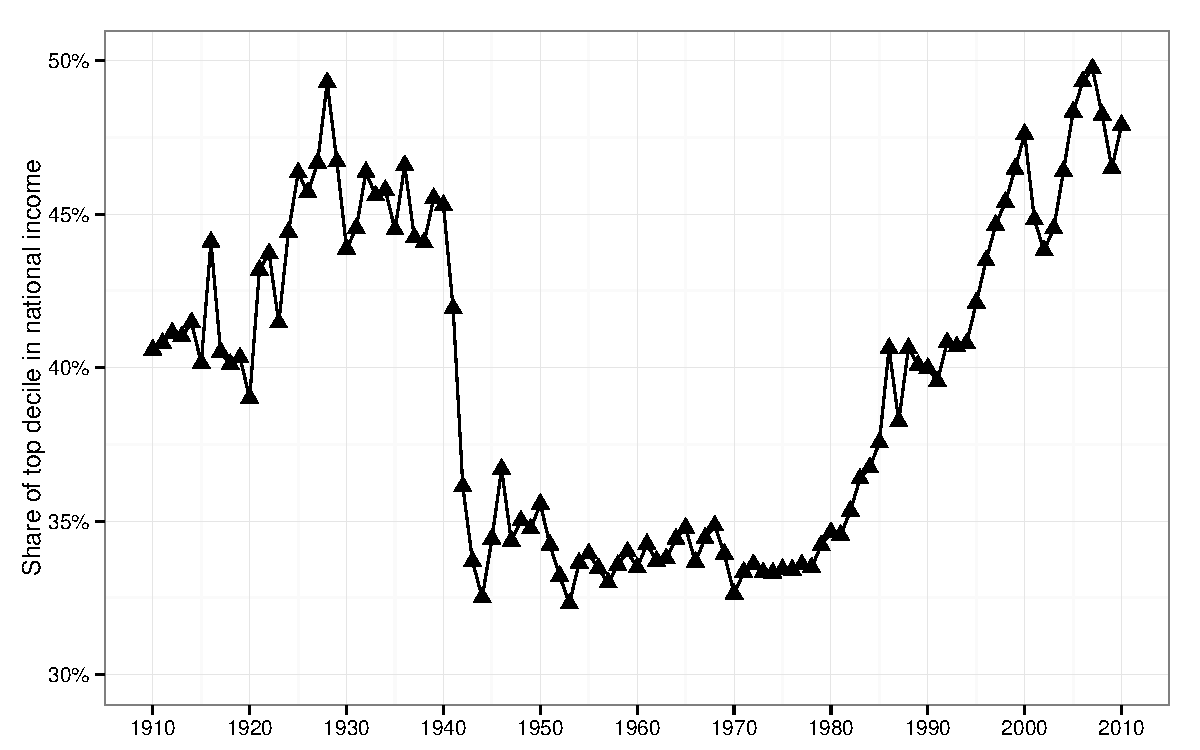
\includegraphics[width=1\linewidth]{figures/bw/Figure_0_1} 

}



\end{knitrout}
\caption{\scriptsize The top decile share in U.S. national income dropped from 45--50\% in the 1910s--1920s to less than 35\% in the 1950s (this is the 1950--1960 fall documented by Kuznets); it then rose from less than 35\% in the 1970s to 45--50\% in the 2000s--2010s.}
\end{minipage}
\end{figure}
\end{frame}
%%%%%%%%%%%%%%%%%%%% Frame Here %%%%%%%%%%%%%%%%%%%%%%%%%%%%%%%%%%%%%%%%%%%%%%%%


%%%%%%%%%%%%%%%%%%%% Frame Here %%%%%%%%%%%%%%%%%%%%%%%%%%%%%%%%%%%%%%%%%%%%%%%%
\begin{frame}[label=Figure_0_2,fragile]
\frametitle{Figure I.2. The capital--income ratio in Europe, 1870--2012}
\begin{figure}[t]
\begin{minipage}[b]{\textwidth}
\centering
\begin{knitrout}\footnotesize
\definecolor{shadecolor}{rgb}{0.969, 0.969, 0.969}\color{fgcolor}

{\centering 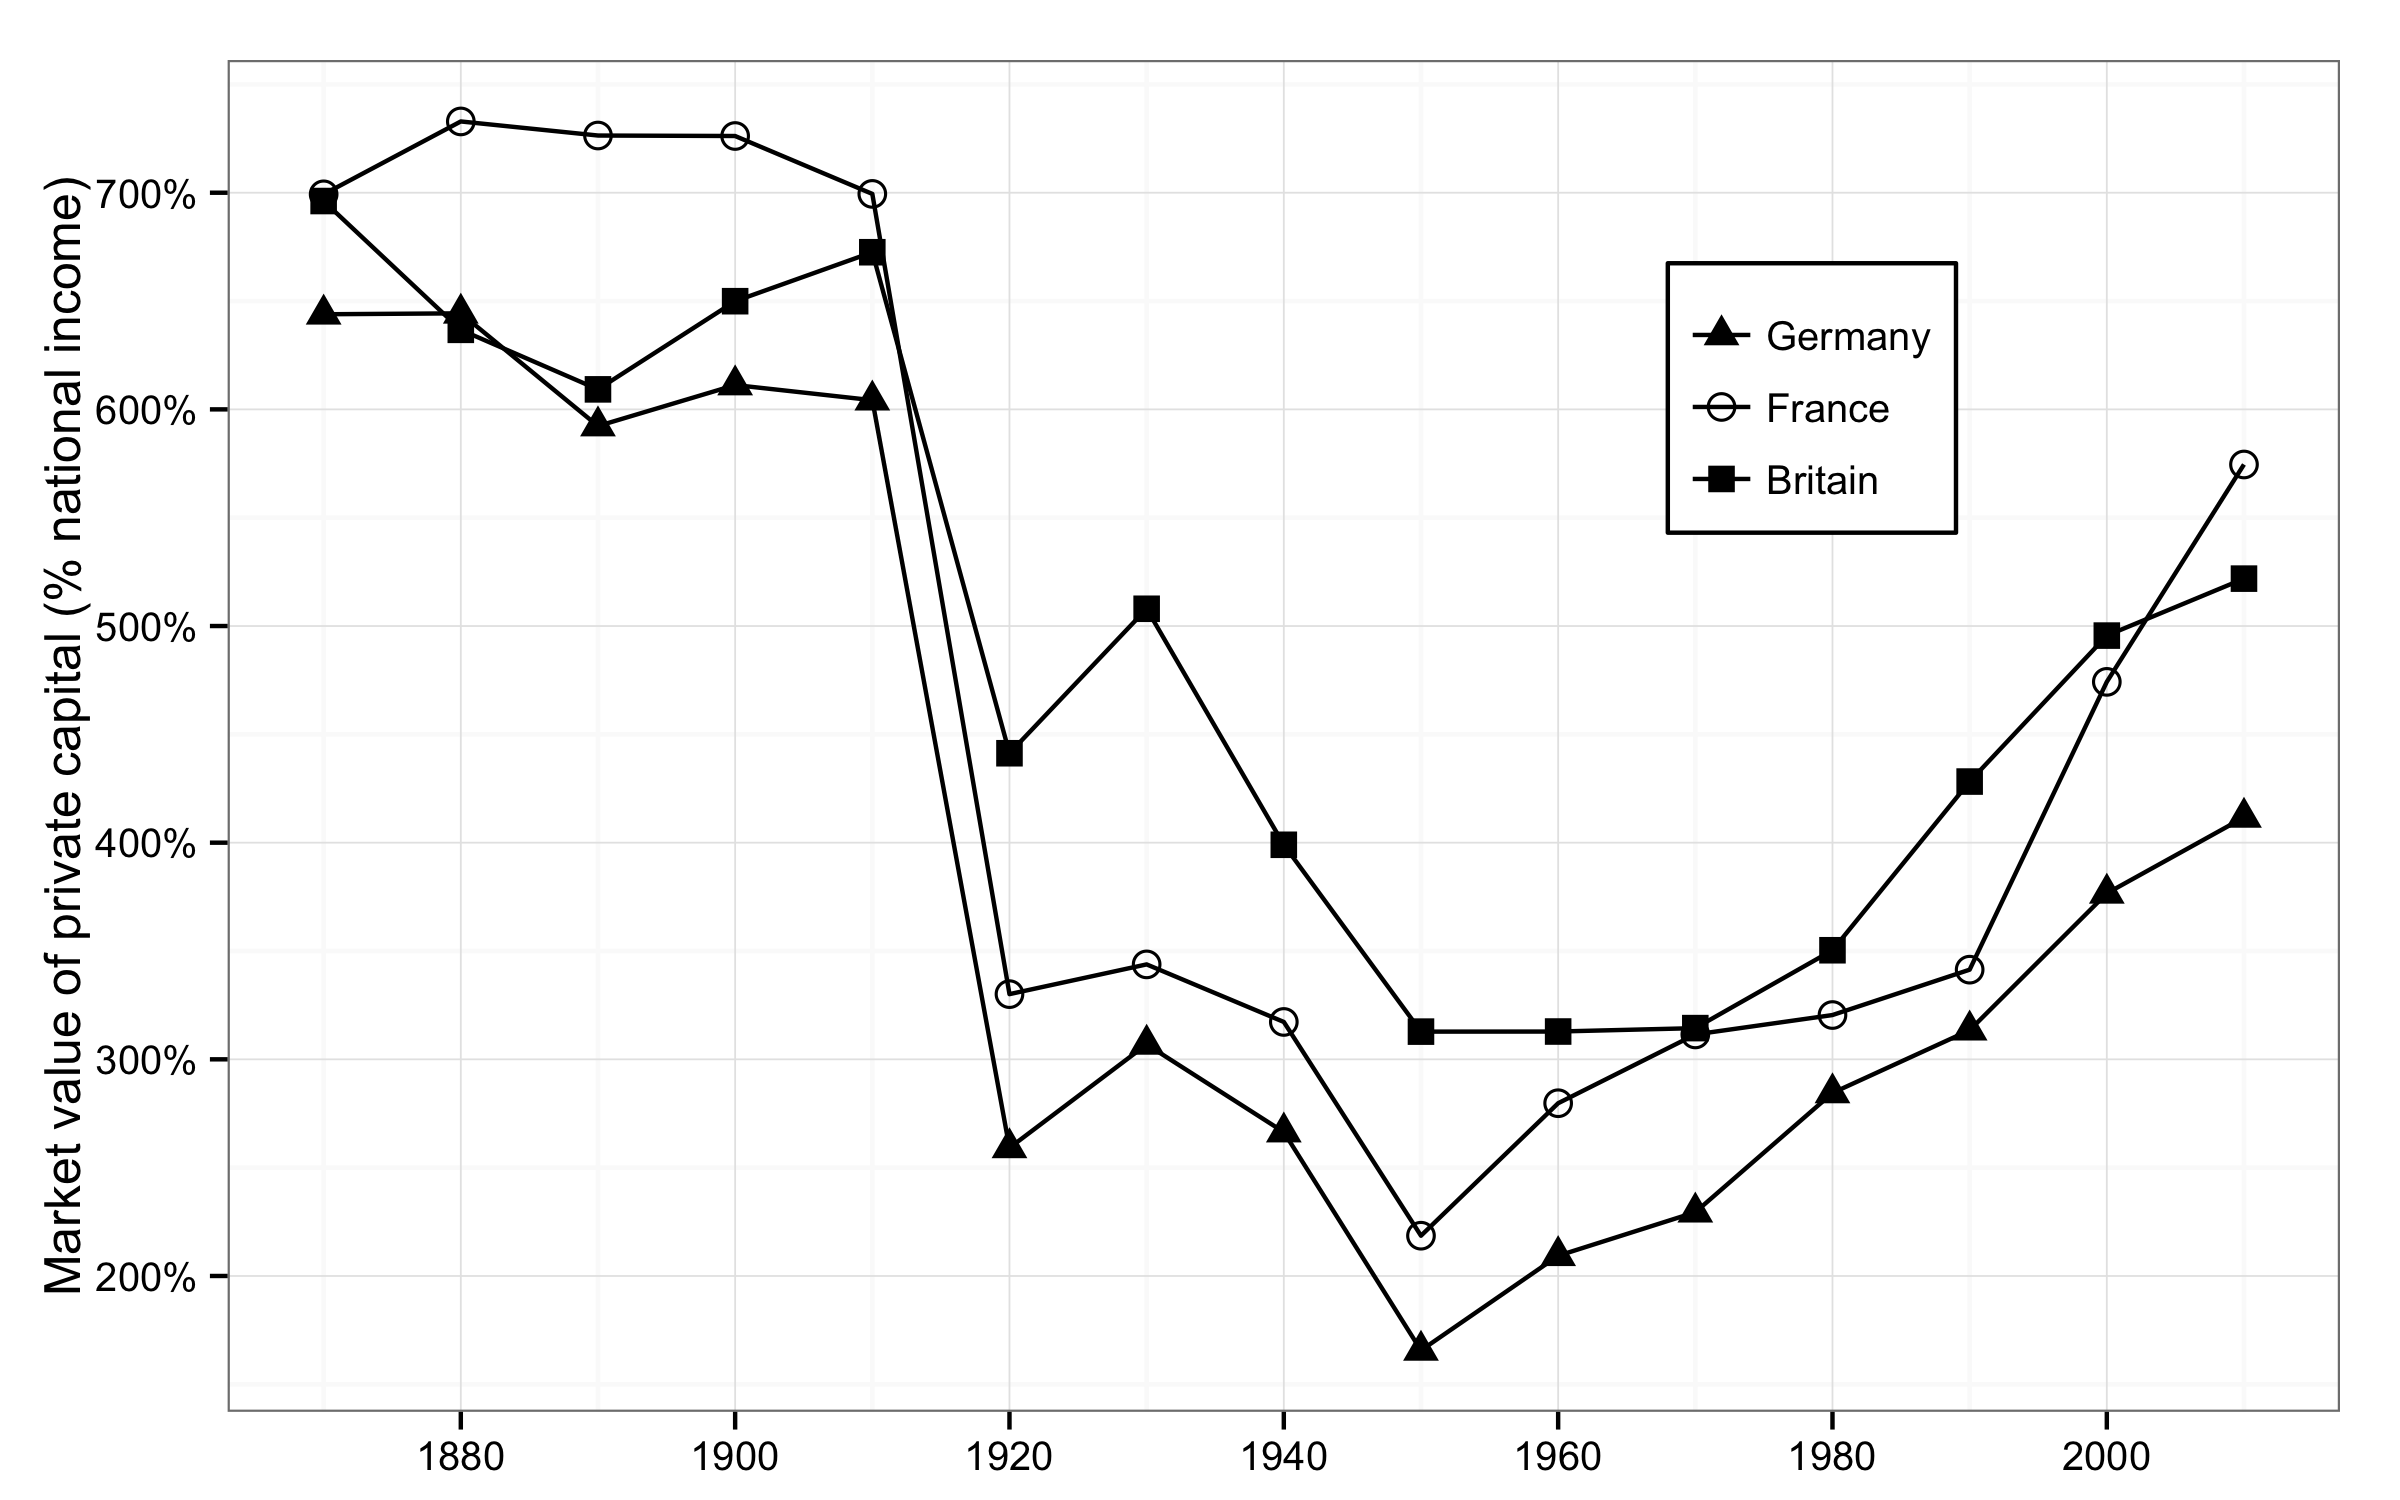
\includegraphics[width=1\linewidth]{figures/bw/Figure_0_2} 

}



\end{knitrout}
\caption{Aggregate private wealth was worth about 6--7 years of national income in Europe in 1910, between 2 and 3 years in 1950, and between 4 and 6 years in 2010.}
\end{minipage}
\end{figure}
\end{frame}
%%%%%%%%%%%%%%%%%%%% Frame Here %%%%%%%%%%%%%%%%%%%%%%%%%%%%%%%%%%%%%%%%%%%%%%%%


%%%%%%%%%%%%%%%%%%%% Frame Here %%%%%%%%%%%%%%%%%%%%%%%%%%%%%%%%%%%%%%%%%%%%%%%%
\begin{frame}[label=Figure_1_1]
\frametitle{Figure 1.1. The distribution of world output, 1700--2012}
\begin{figure}[t]
\begin{minipage}[b]{\textwidth}
\centering
\begin{knitrout}\footnotesize
\definecolor{shadecolor}{rgb}{0.969, 0.969, 0.969}\color{fgcolor}

{\centering 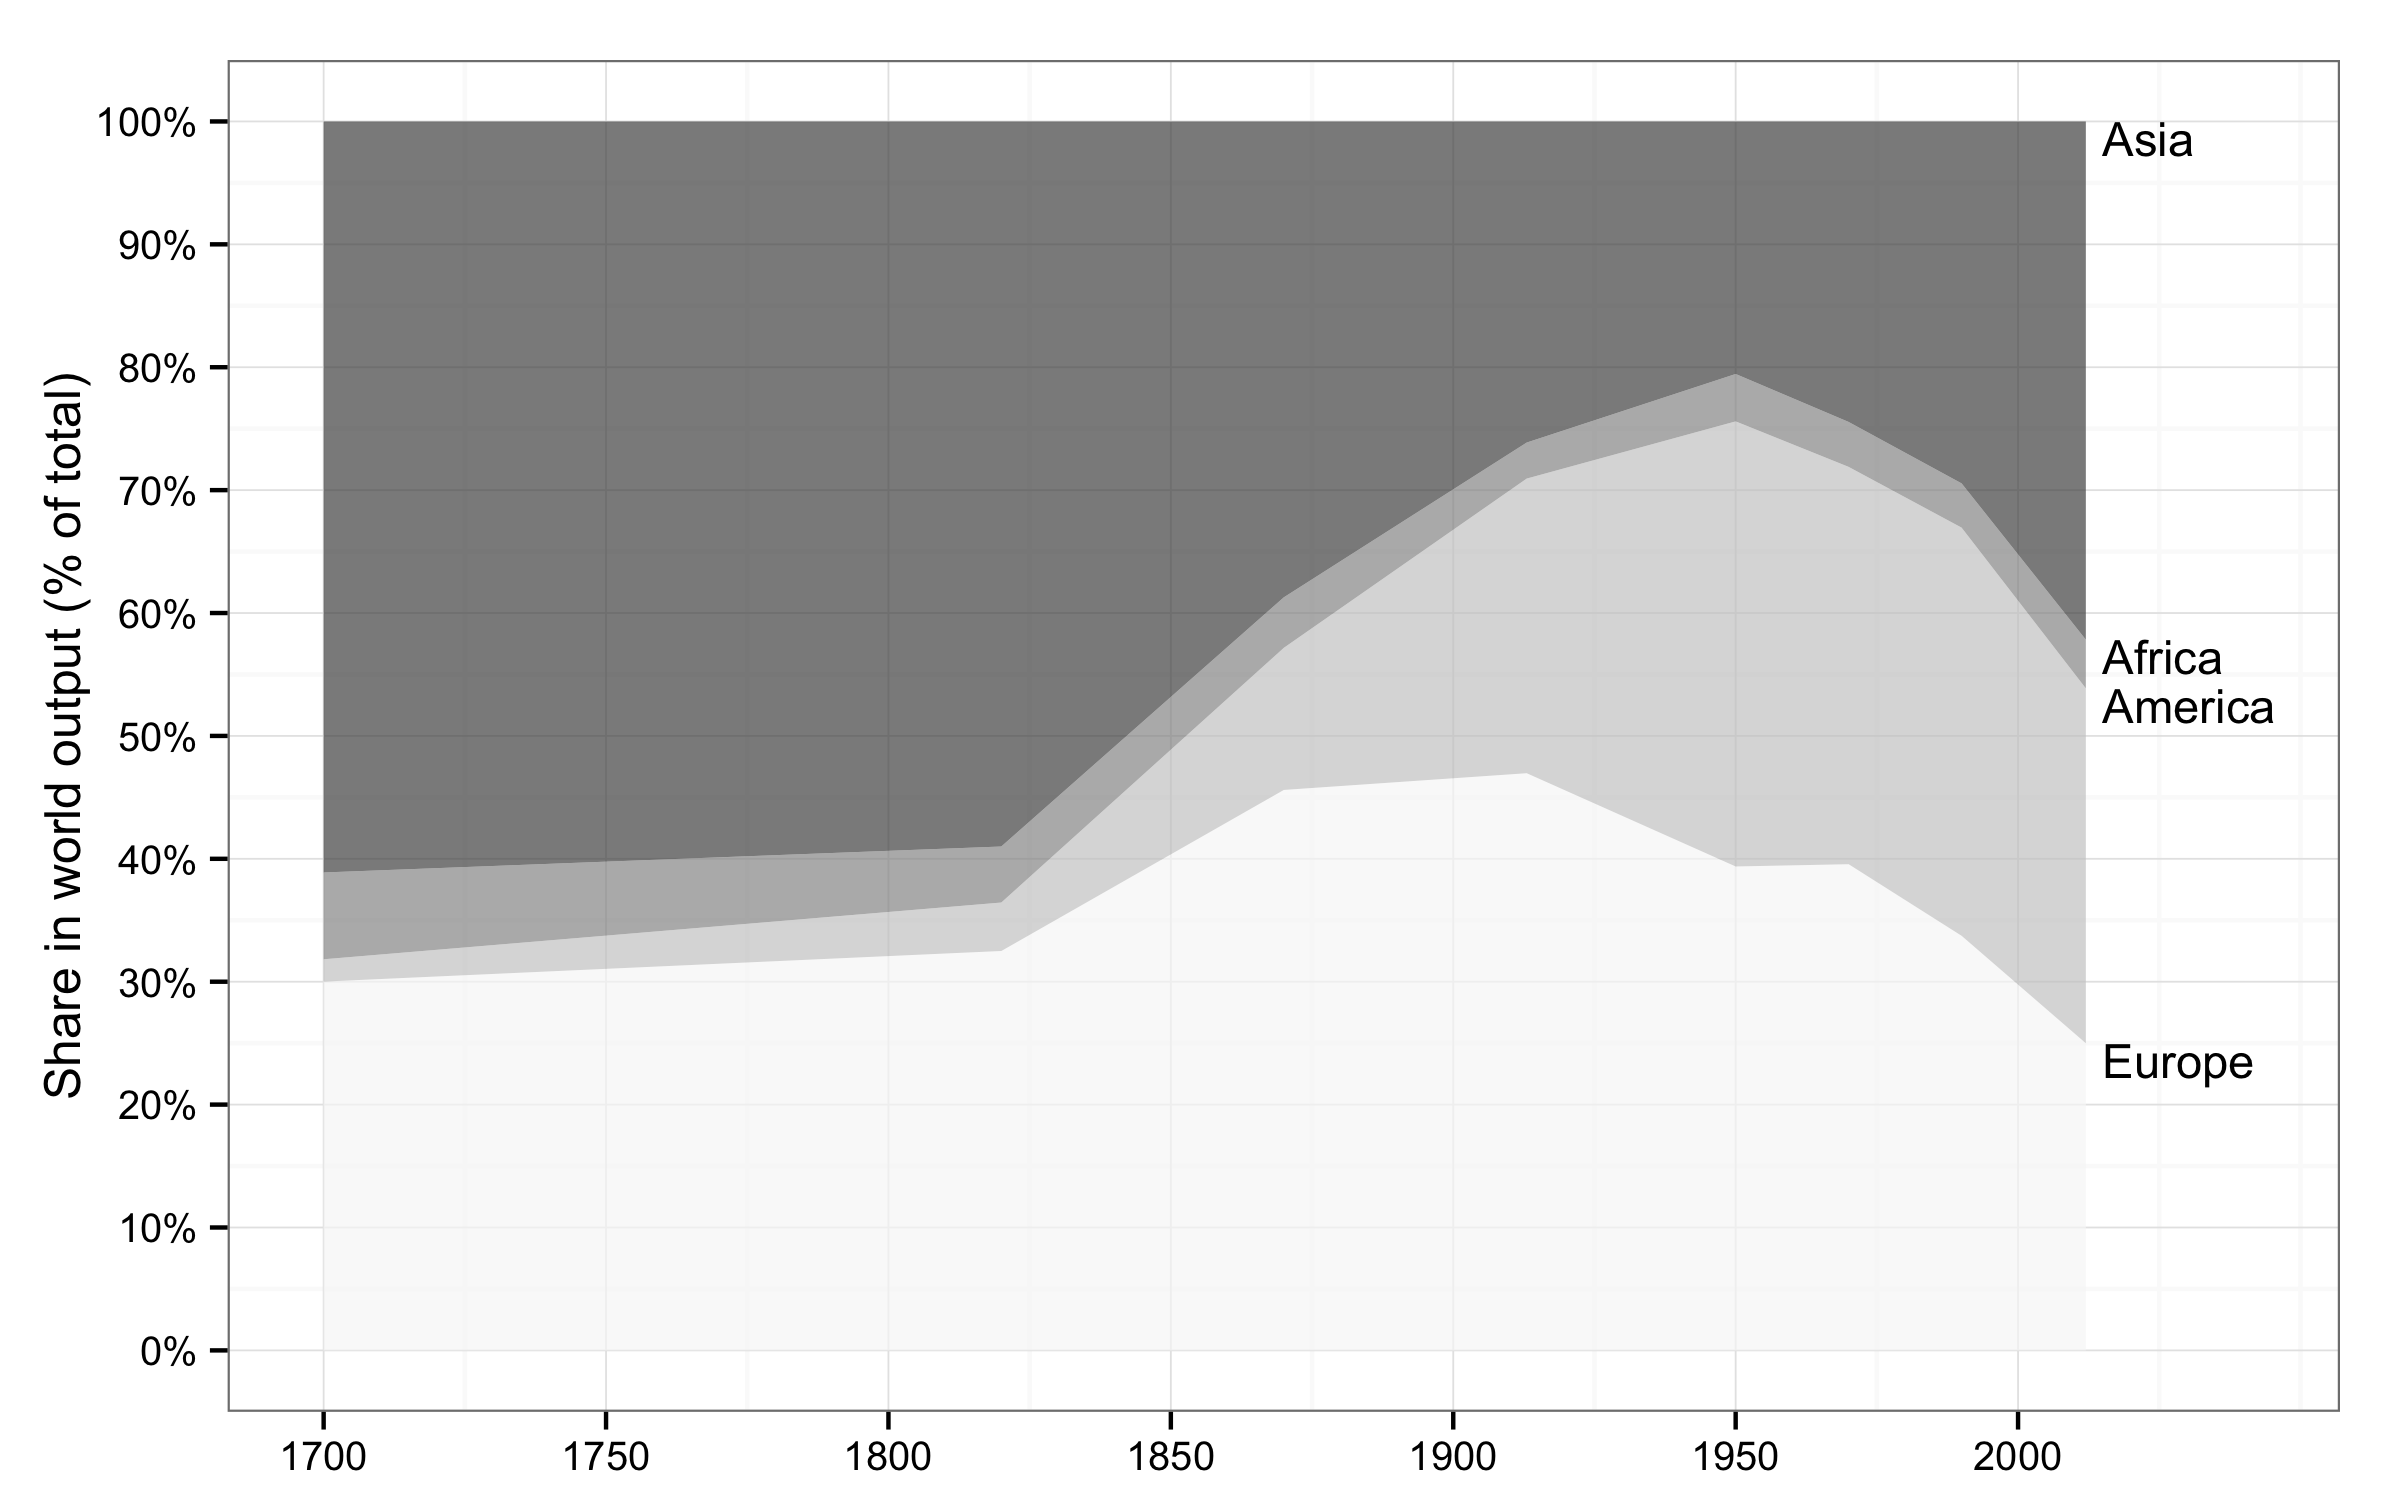
\includegraphics[width=1\linewidth]{figures/bw/Figure_1_1} 

}



\end{knitrout}
\caption{Europe's GDP made 47 percent of world GDP in 1913, down to 25 percent in 2012.}
\end{minipage}
\end{figure}
\end{frame}
%%%%%%%%%%%%%%%%%%%% Frame Here %%%%%%%%%%%%%%%%%%%%%%%%%%%%%%%%%%%%%%%%%%%%%%%%


%%%%%%%%%%%%%%%%%%%% Frame Here %%%%%%%%%%%%%%%%%%%%%%%%%%%%%%%%%%%%%%%%%%%%%%%%
\begin{frame}[label=Figure_1_1b]
\frametitle{Figure 1.1. The distribution of world output, 1700--2012}
\begin{figure}[t]
\begin{minipage}[b]{\textwidth}
\centering
\begin{knitrout}\footnotesize
\definecolor{shadecolor}{rgb}{0.969, 0.969, 0.969}\color{fgcolor}

{\centering 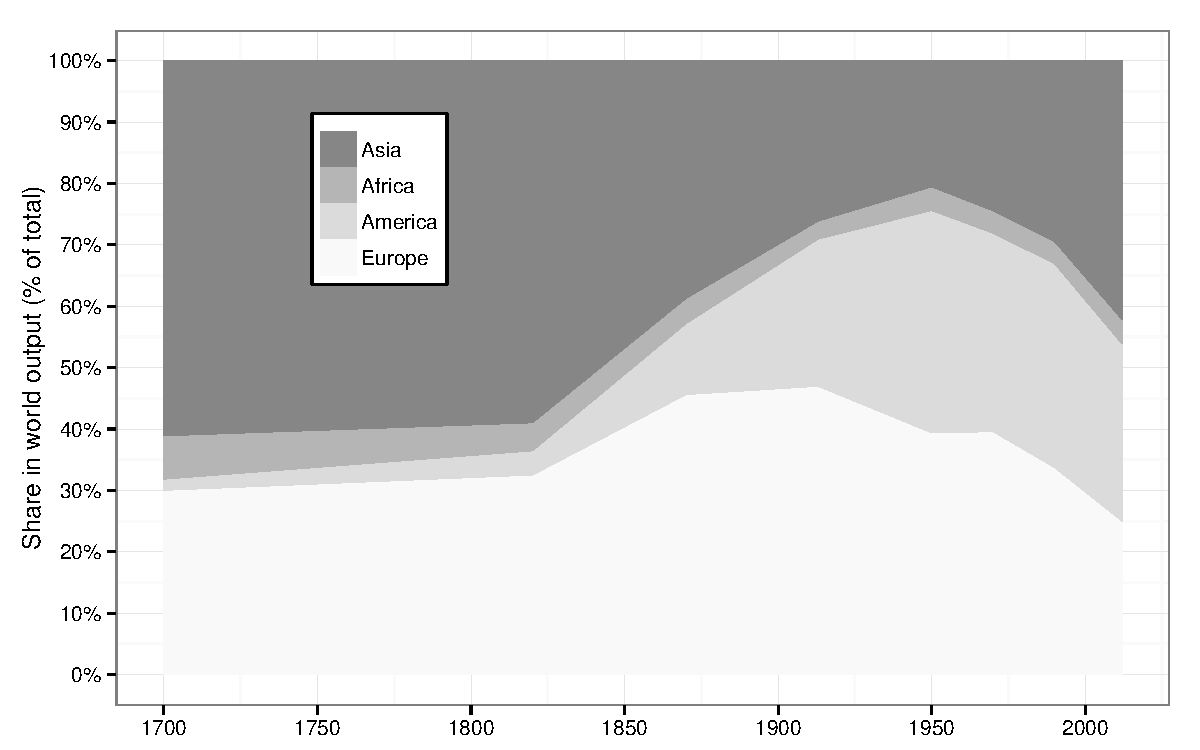
\includegraphics[width=1\linewidth]{figures/bw/Figure_1_1b} 

}



\end{knitrout}
\caption{Europe's GDP made 47 percent of world GDP in 1913, down to 25 percent in 2012.}
\end{minipage}
\end{figure}
\end{frame}
%%%%%%%%%%%%%%%%%%%% Frame Here %%%%%%%%%%%%%%%%%%%%%%%%%%%%%%%%%%%%%%%%%%%%%%%%


%%%%%%%%%%%%%%%%%%%% Frame Here %%%%%%%%%%%%%%%%%%%%%%%%%%%%%%%%%%%%%%%%%%%%%%%%
\begin{frame}[label=Figure_1_2]
\frametitle{Figure 1.2. The distribution of world population, 1700--2012}
\begin{figure}[t]
\begin{minipage}[b]{\textwidth}
\centering
\begin{knitrout}\footnotesize
\definecolor{shadecolor}{rgb}{0.969, 0.969, 0.969}\color{fgcolor}

{\centering 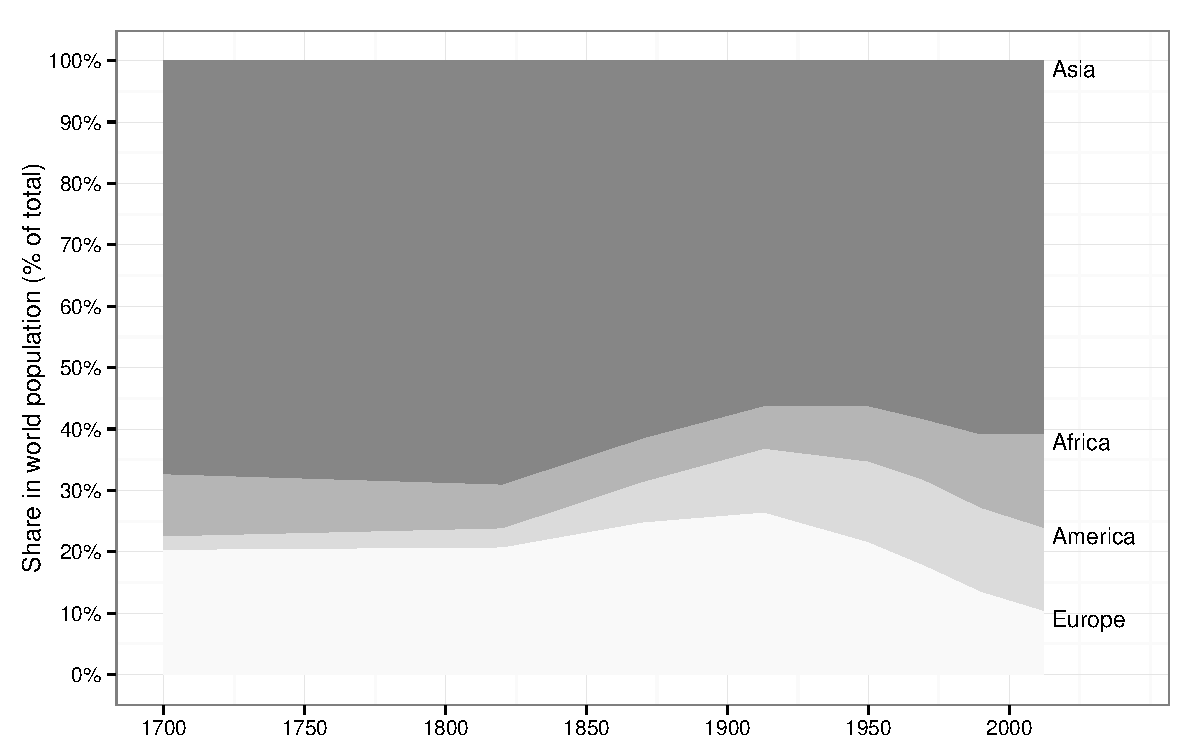
\includegraphics[width=1\linewidth]{figures/bw/Figure_1_2} 

}



\end{knitrout}
\caption{Europe's population made 26 percent of world population in 1913, down to 10 percent in 2012.}
\end{minipage}
\end{figure}
\end{frame}
%%%%%%%%%%%%%%%%%%%% Frame Here %%%%%%%%%%%%%%%%%%%%%%%%%%%%%%%%%%%%%%%%%%%%%%%%


%%%%%%%%%%%%%%%%%%%% Frame Here %%%%%%%%%%%%%%%%%%%%%%%%%%%%%%%%%%%%%%%%%%%%%%%%
\begin{frame}[label=Figure_1_2b]
\frametitle{Figure 1.2. The distribution of world population, 1700--2012}
\begin{figure}[t]
\begin{minipage}[b]{\textwidth}
\centering
\begin{knitrout}\footnotesize
\definecolor{shadecolor}{rgb}{0.969, 0.969, 0.969}\color{fgcolor}

{\centering 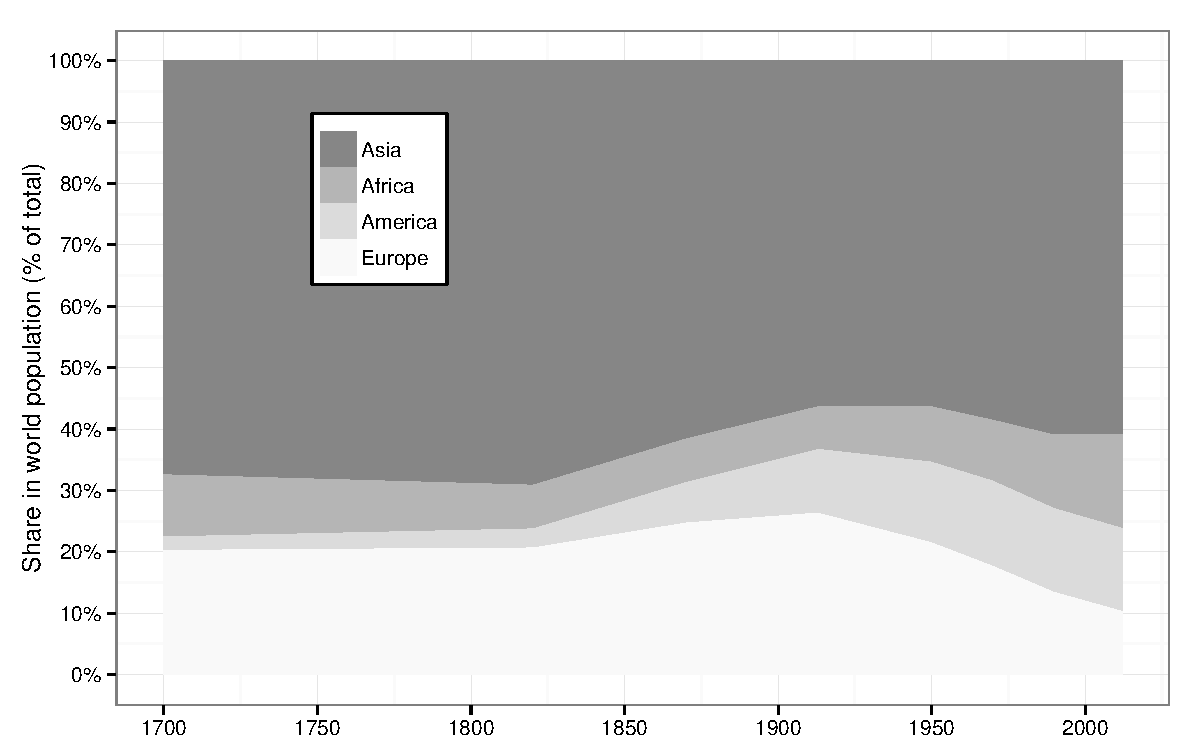
\includegraphics[width=1\linewidth]{figures/bw/Figure_1_2b} 

}



\end{knitrout}
\caption{Europe's population made 26 percent of world population in 1913, down to 10 percent in 2012.}
\end{minipage}
\end{figure}
\end{frame}
%%%%%%%%%%%%%%%%%%%% Frame Here %%%%%%%%%%%%%%%%%%%%%%%%%%%%%%%%%%%%%%%%%%%%%%%%


%%%%%%%%%%%%%%%%%%%% Frame Here %%%%%%%%%%%%%%%%%%%%%%%%%%%%%%%%%%%%%%%%%%%%%%%%
\begin{frame}[label=Figure_1_3,fragile]
\frametitle{Figure 1.3. Global Inequality, 1700--2012}
\begin{figure}[t]
\begin{minipage}[b]{\textwidth}
\centering
\begin{knitrout}\footnotesize
\definecolor{shadecolor}{rgb}{0.969, 0.969, 0.969}\color{fgcolor}

{\centering 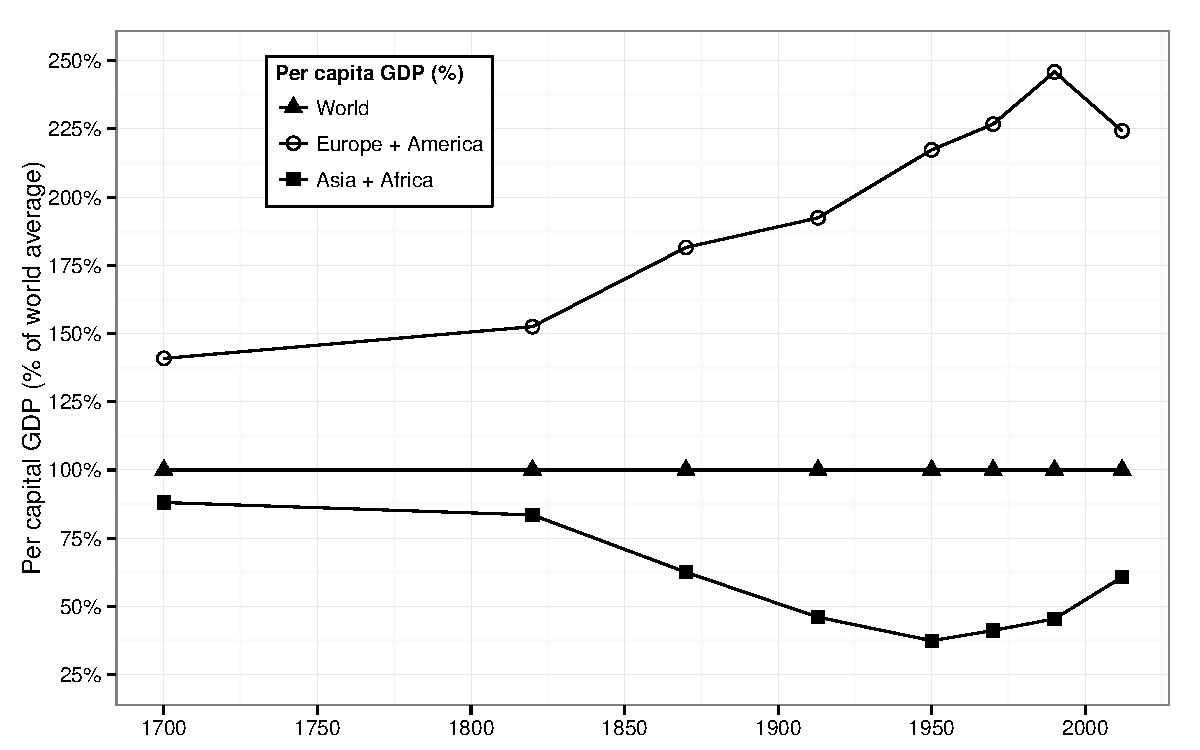
\includegraphics[width=1\linewidth]{figures/bw/Figure_1_3} 

}



\end{knitrout}
\caption{Per capita GDP in Asia--Africa went from 37 percent of world average in 1950 to 61 percent in 2012. Divergence then convergence?}
\end{minipage}
\end{figure}
\end{frame}
%%%%%%%%%%%%%%%%%%%% Frame Here %%%%%%%%%%%%%%%%%%%%%%%%%%%%%%%%%%%%%%%%%%%%%%%%


%%%%%%%%%%%%%%%%%%%% Frame Here %%%%%%%%%%%%%%%%%%%%%%%%%%%%%%%%%%%%%%%%%%%%%%%%
\begin{frame}[label=Figure_1_4,fragile]
\frametitle{Figure 1.4. Exchange rate and purchasing power parity: euro/dollar}
\begin{figure}[t]
\begin{minipage}[b]{\textwidth}
\centering
\begin{knitrout}\footnotesize
\definecolor{shadecolor}{rgb}{0.969, 0.969, 0.969}\color{fgcolor}

{\centering 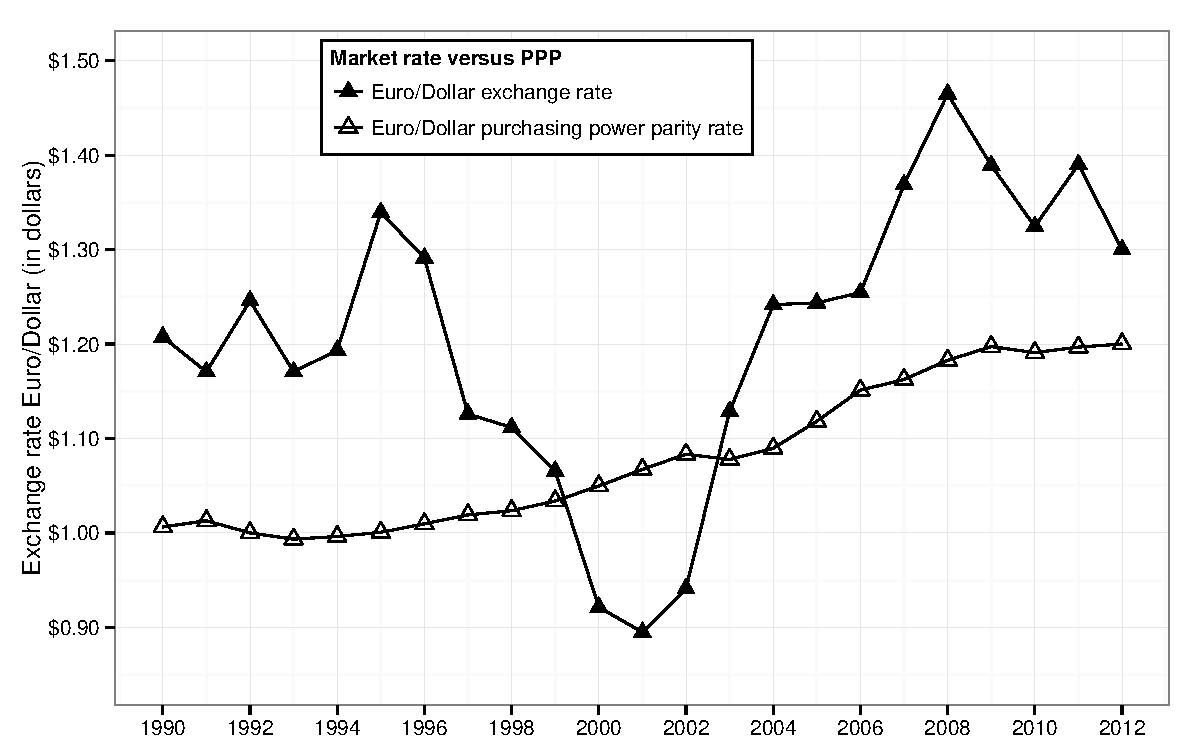
\includegraphics[width=1\linewidth]{figures/bw/Figure_1_4} 

}



\end{knitrout}
\caption{In 2012, 1 euro was worth \$1.30 according to current exchange rate, but \$1.20 in purchasing power parity.}
\end{minipage}
\end{figure}
\end{frame}
%%%%%%%%%%%%%%%%%%%% Frame Here %%%%%%%%%%%%%%%%%%%%%%%%%%%%%%%%%%%%%%%%%%%%%%%%


%%%%%%%%%%%%%%%%%%%% Frame Here %%%%%%%%%%%%%%%%%%%%%%%%%%%%%%%%%%%%%%%%%%%%%%%%
\begin{frame}[label=Figure_1_5,fragile]
\frametitle{Figure 1.5. Exchange rate and purchasing power parity: euro/yuan}
\begin{figure}[t]
\begin{minipage}[b]{\textwidth}
\centering
\begin{knitrout}\footnotesize
\definecolor{shadecolor}{rgb}{0.969, 0.969, 0.969}\color{fgcolor}

{\centering 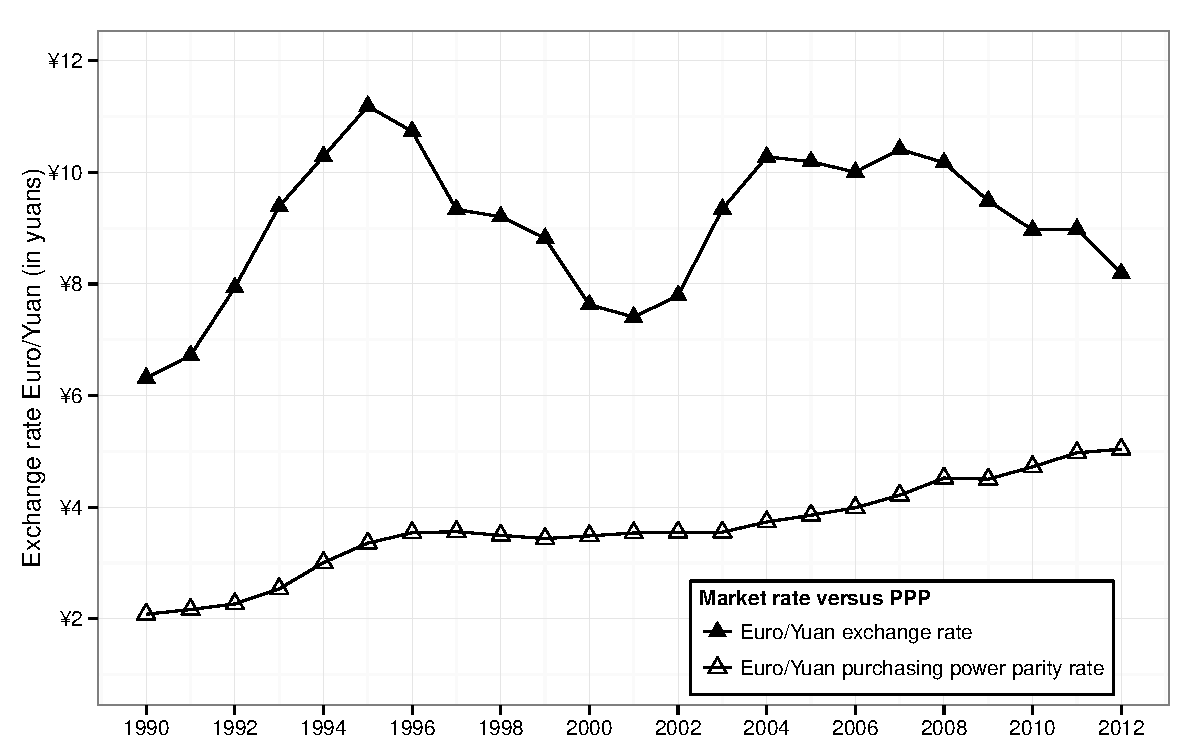
\includegraphics[width=1\linewidth]{figures/bw/Figure_1_5} 

}



\end{knitrout}
\caption{In 2012, 1 euro was worth 8 yuan according to current exchange rate, but 5 yuan in purchasing power parity.}
\end{minipage}
\end{figure}
\end{frame}
%%%%%%%%%%%%%%%%%%%% Frame Here %%%%%%%%%%%%%%%%%%%%%%%%%%%%%%%%%%%%%%%%%%%%%%%%


%%%%%%%%%%%%%%%%%%%% Frame Here %%%%%%%%%%%%%%%%%%%%%%%%%%%%%%%%%%%%%%%%%%%%%%%%
\begin{frame}[label=Figure_S1_4a,fragile]
\frametitle{Figure S1.4a. Exchange rate and purchasing power parity : euro/rupee}
\begin{figure}[t]
\begin{minipage}[b]{\textwidth}
\centering
\begin{knitrout}\footnotesize
\definecolor{shadecolor}{rgb}{0.969, 0.969, 0.969}\color{fgcolor}

{\centering 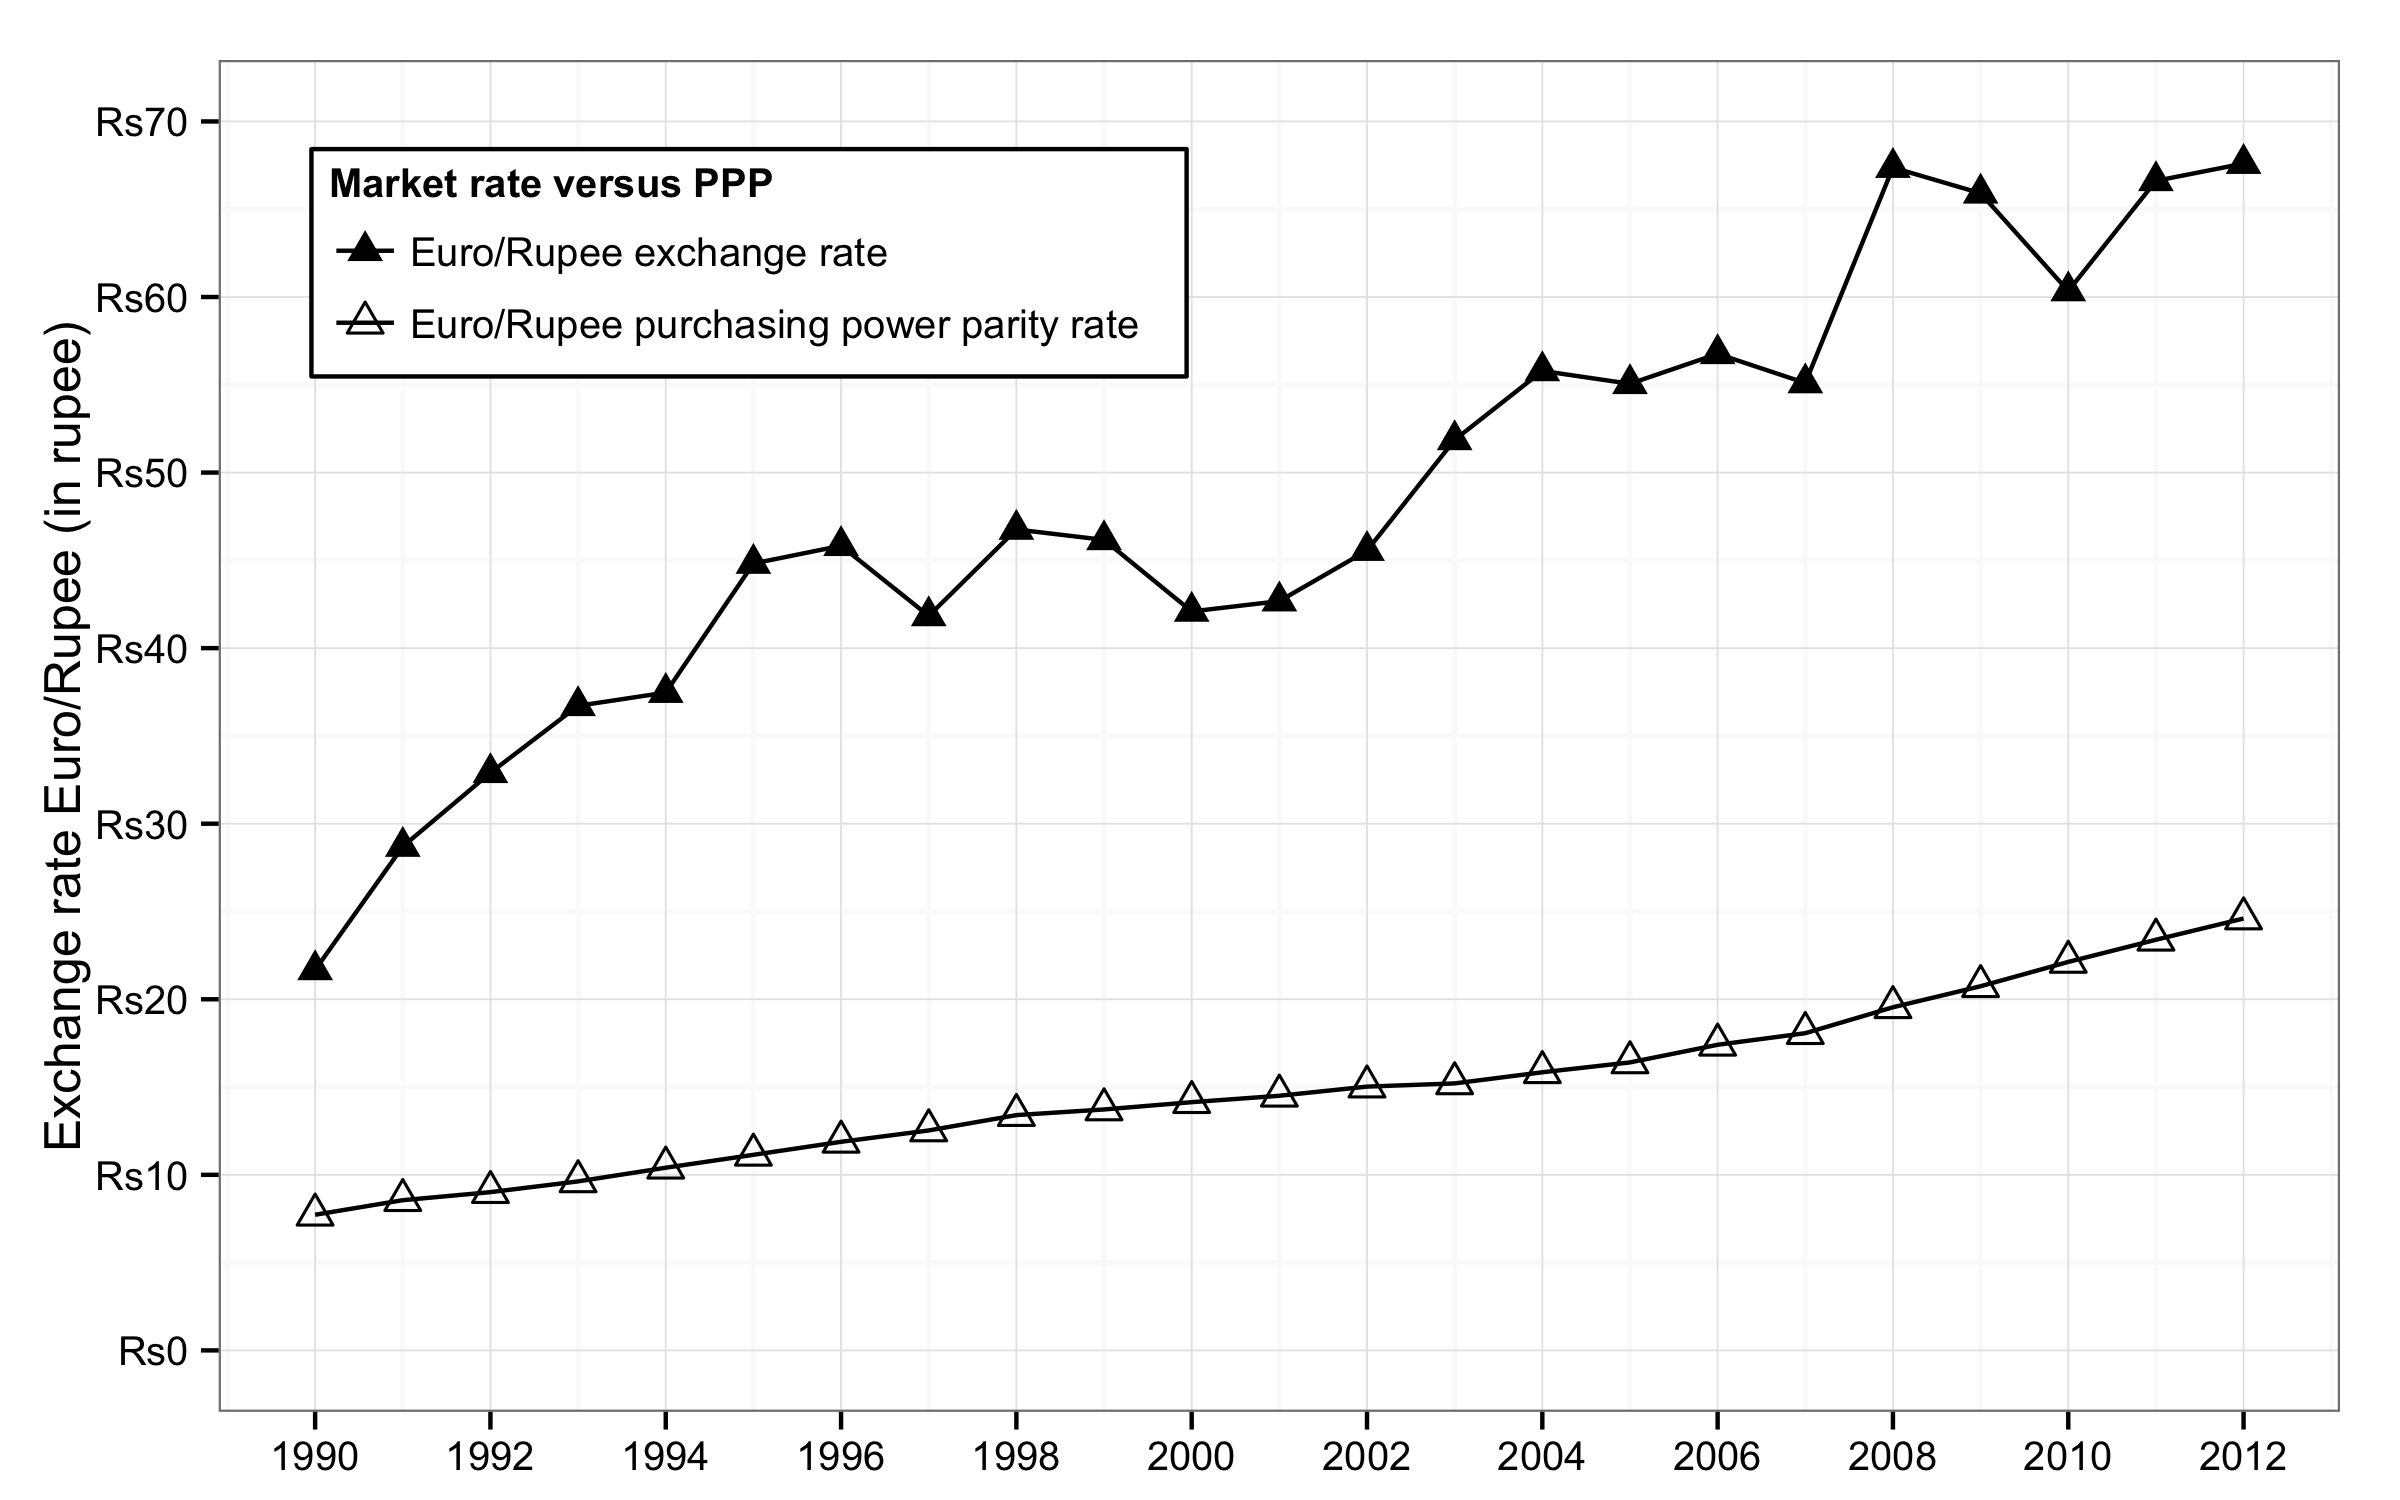
\includegraphics[width=1\linewidth]{figures/bw/Figure_S1_4a} 

}



\end{knitrout}
\caption{In 2012, 1 euro was worth around 70 rupees according to current exchange rate, but 25 rupees in purchasing power parity.}
\end{minipage}
\end{figure}
\end{frame}
%%%%%%%%%%%%%%%%%%%% Frame Here %%%%%%%%%%%%%%%%%%%%%%%%%%%%%%%%%%%%%%%%%%%%%%%%


%%%%%%%%%%%%%%%%%%%% Frame Here %%%%%%%%%%%%%%%%%%%%%%%%%%%%%%%%%%%%%%%%%%%%%%%%
\begin{frame}[label=Figure_S1_4b,fragile]
\frametitle{Figure S1.4b. Exchange rate and purchasing power parity : euro/yen}
\begin{figure}[t]
\begin{minipage}[b]{\textwidth}
\centering
\begin{knitrout}\footnotesize
\definecolor{shadecolor}{rgb}{0.969, 0.969, 0.969}\color{fgcolor}

{\centering 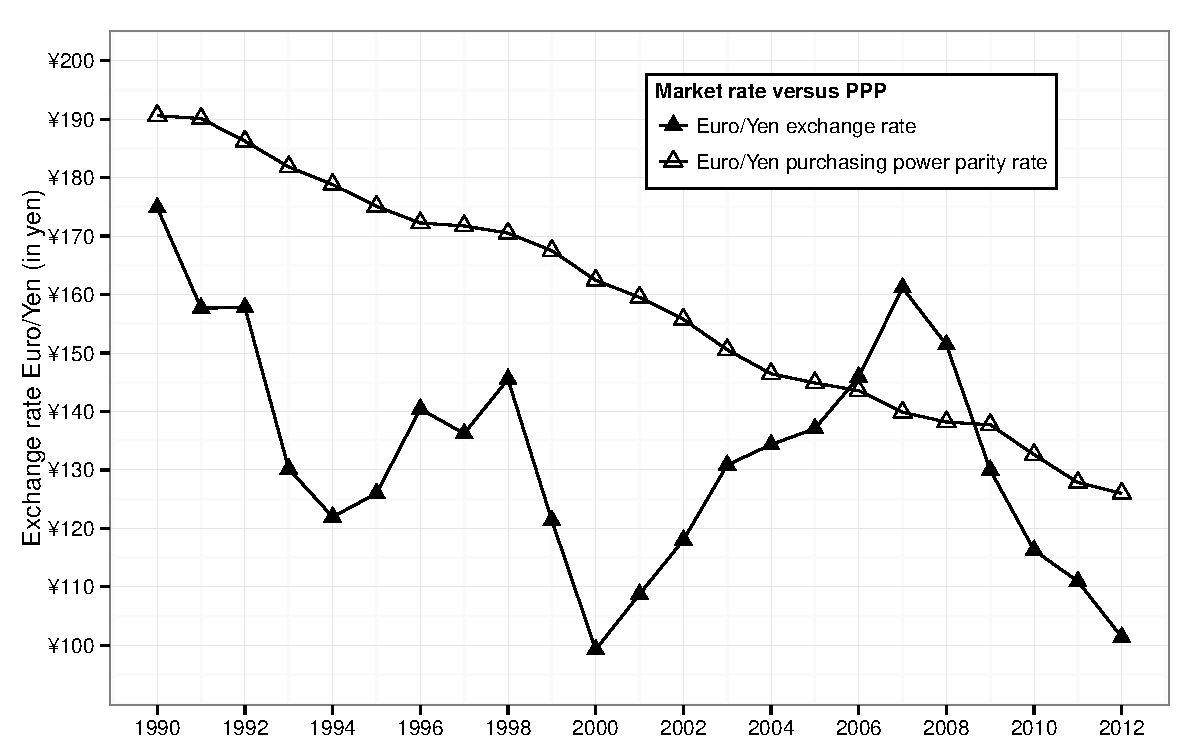
\includegraphics[width=1\linewidth]{figures/bw/Figure_S1_4b} 

}



\end{knitrout}
\caption{In 2012, 1 euro was worth around 100 yens according to current exchange rate, but 125 yens in purchasing power parity.}
\end{minipage}
\end{figure}
\end{frame}
%%%%%%%%%%%%%%%%%%%% Frame Here %%%%%%%%%%%%%%%%%%%%%%%%%%%%%%%%%%%%%%%%%%%%%%%%


%%%%%%%%%%%%%%%%%%%% Frame Here %%%%%%%%%%%%%%%%%%%%%%%%%%%%%%%%%%%%%%%%%%%%%%%%
\begin{frame}[label=Figure_S1_5a,fragile]
\frametitle{Figure S1.5a. Exchange rate and purchasing power parity : dollar/yuan}
\begin{figure}[t]
\begin{minipage}[b]{\textwidth}
\centering
\begin{knitrout}\footnotesize
\definecolor{shadecolor}{rgb}{0.969, 0.969, 0.969}\color{fgcolor}

{\centering 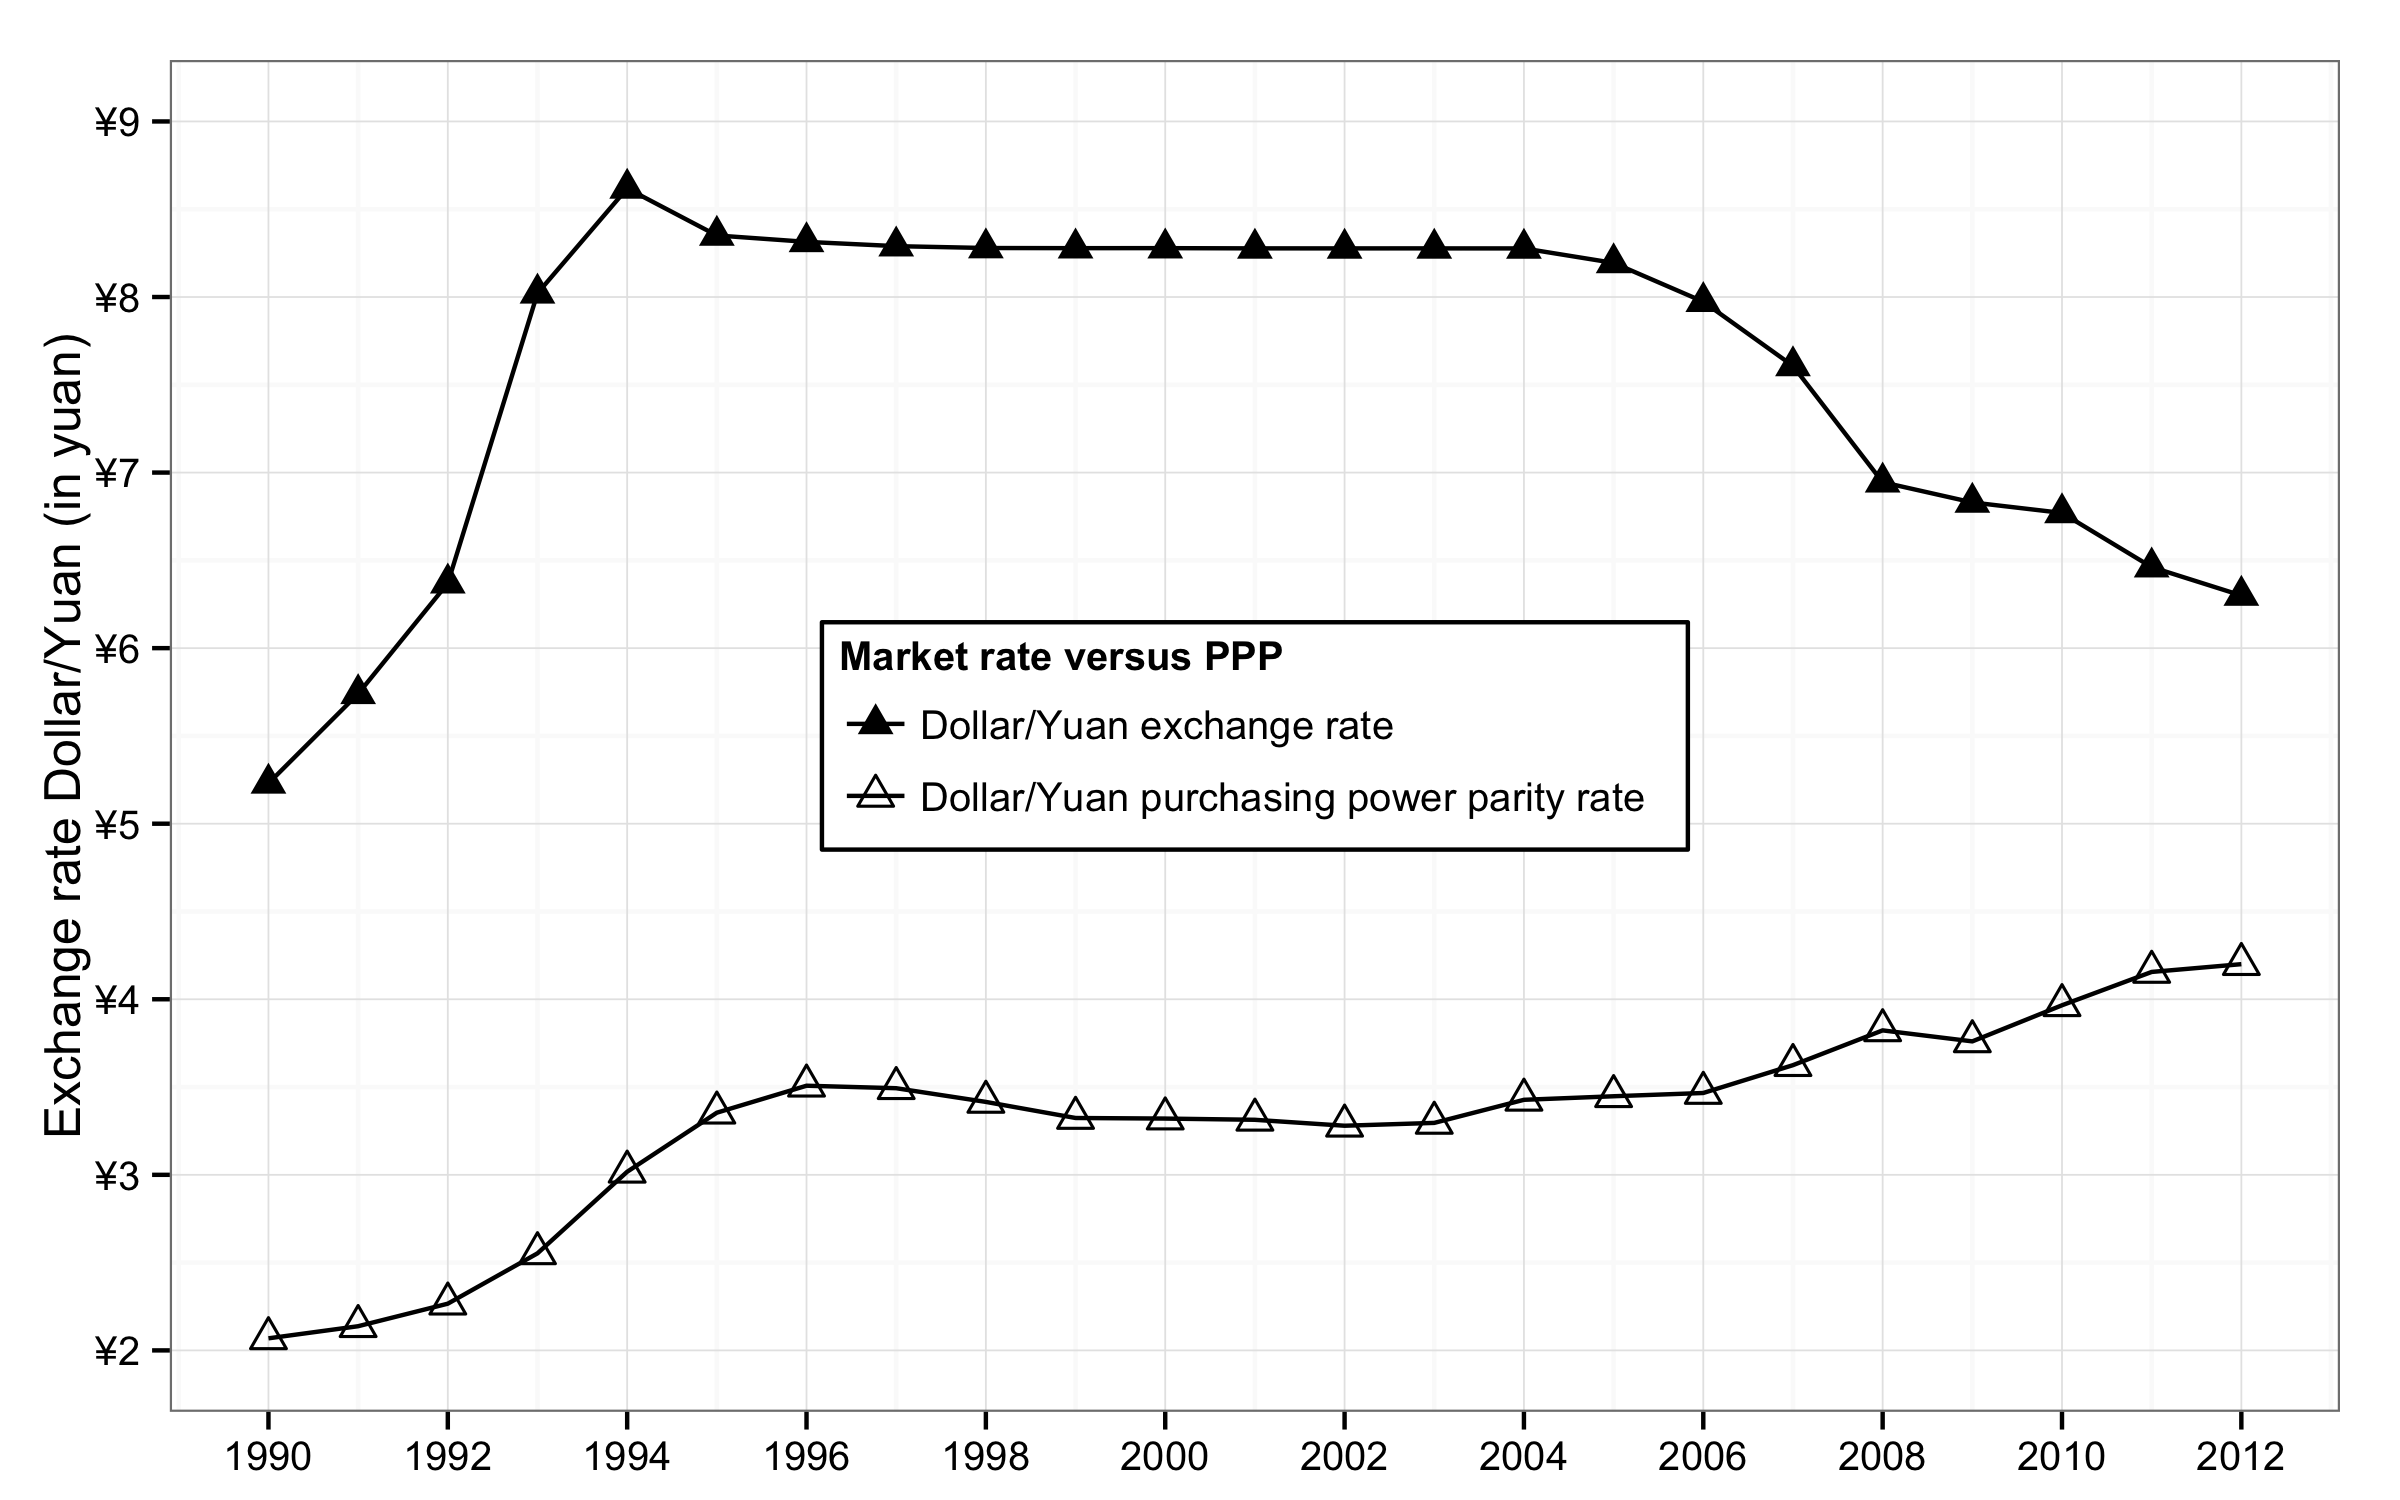
\includegraphics[width=1\linewidth]{figures/bw/Figure_S1_5a} 

}



\end{knitrout}
\caption{In 2012, 1 dollar was worth around 6 yuans according to current exchange rate, but 4 yuans in purchasing power parity.}
\end{minipage}
\end{figure}
\end{frame}
%%%%%%%%%%%%%%%%%%%% Frame Here %%%%%%%%%%%%%%%%%%%%%%%%%%%%%%%%%%%%%%%%%%%%%%%%


%%%%%%%%%%%%%%%%%%%% Frame Here %%%%%%%%%%%%%%%%%%%%%%%%%%%%%%%%%%%%%%%%%%%%%%%%
\begin{frame}[label=Figure_S1_5b,fragile]
\frametitle{Figure S1.5b. Exchange rate and purchasing power parity : dollar/rupee}
\begin{figure}[t]
\begin{minipage}[b]{\textwidth}
\centering
\begin{knitrout}\footnotesize
\definecolor{shadecolor}{rgb}{0.969, 0.969, 0.969}\color{fgcolor}

{\centering 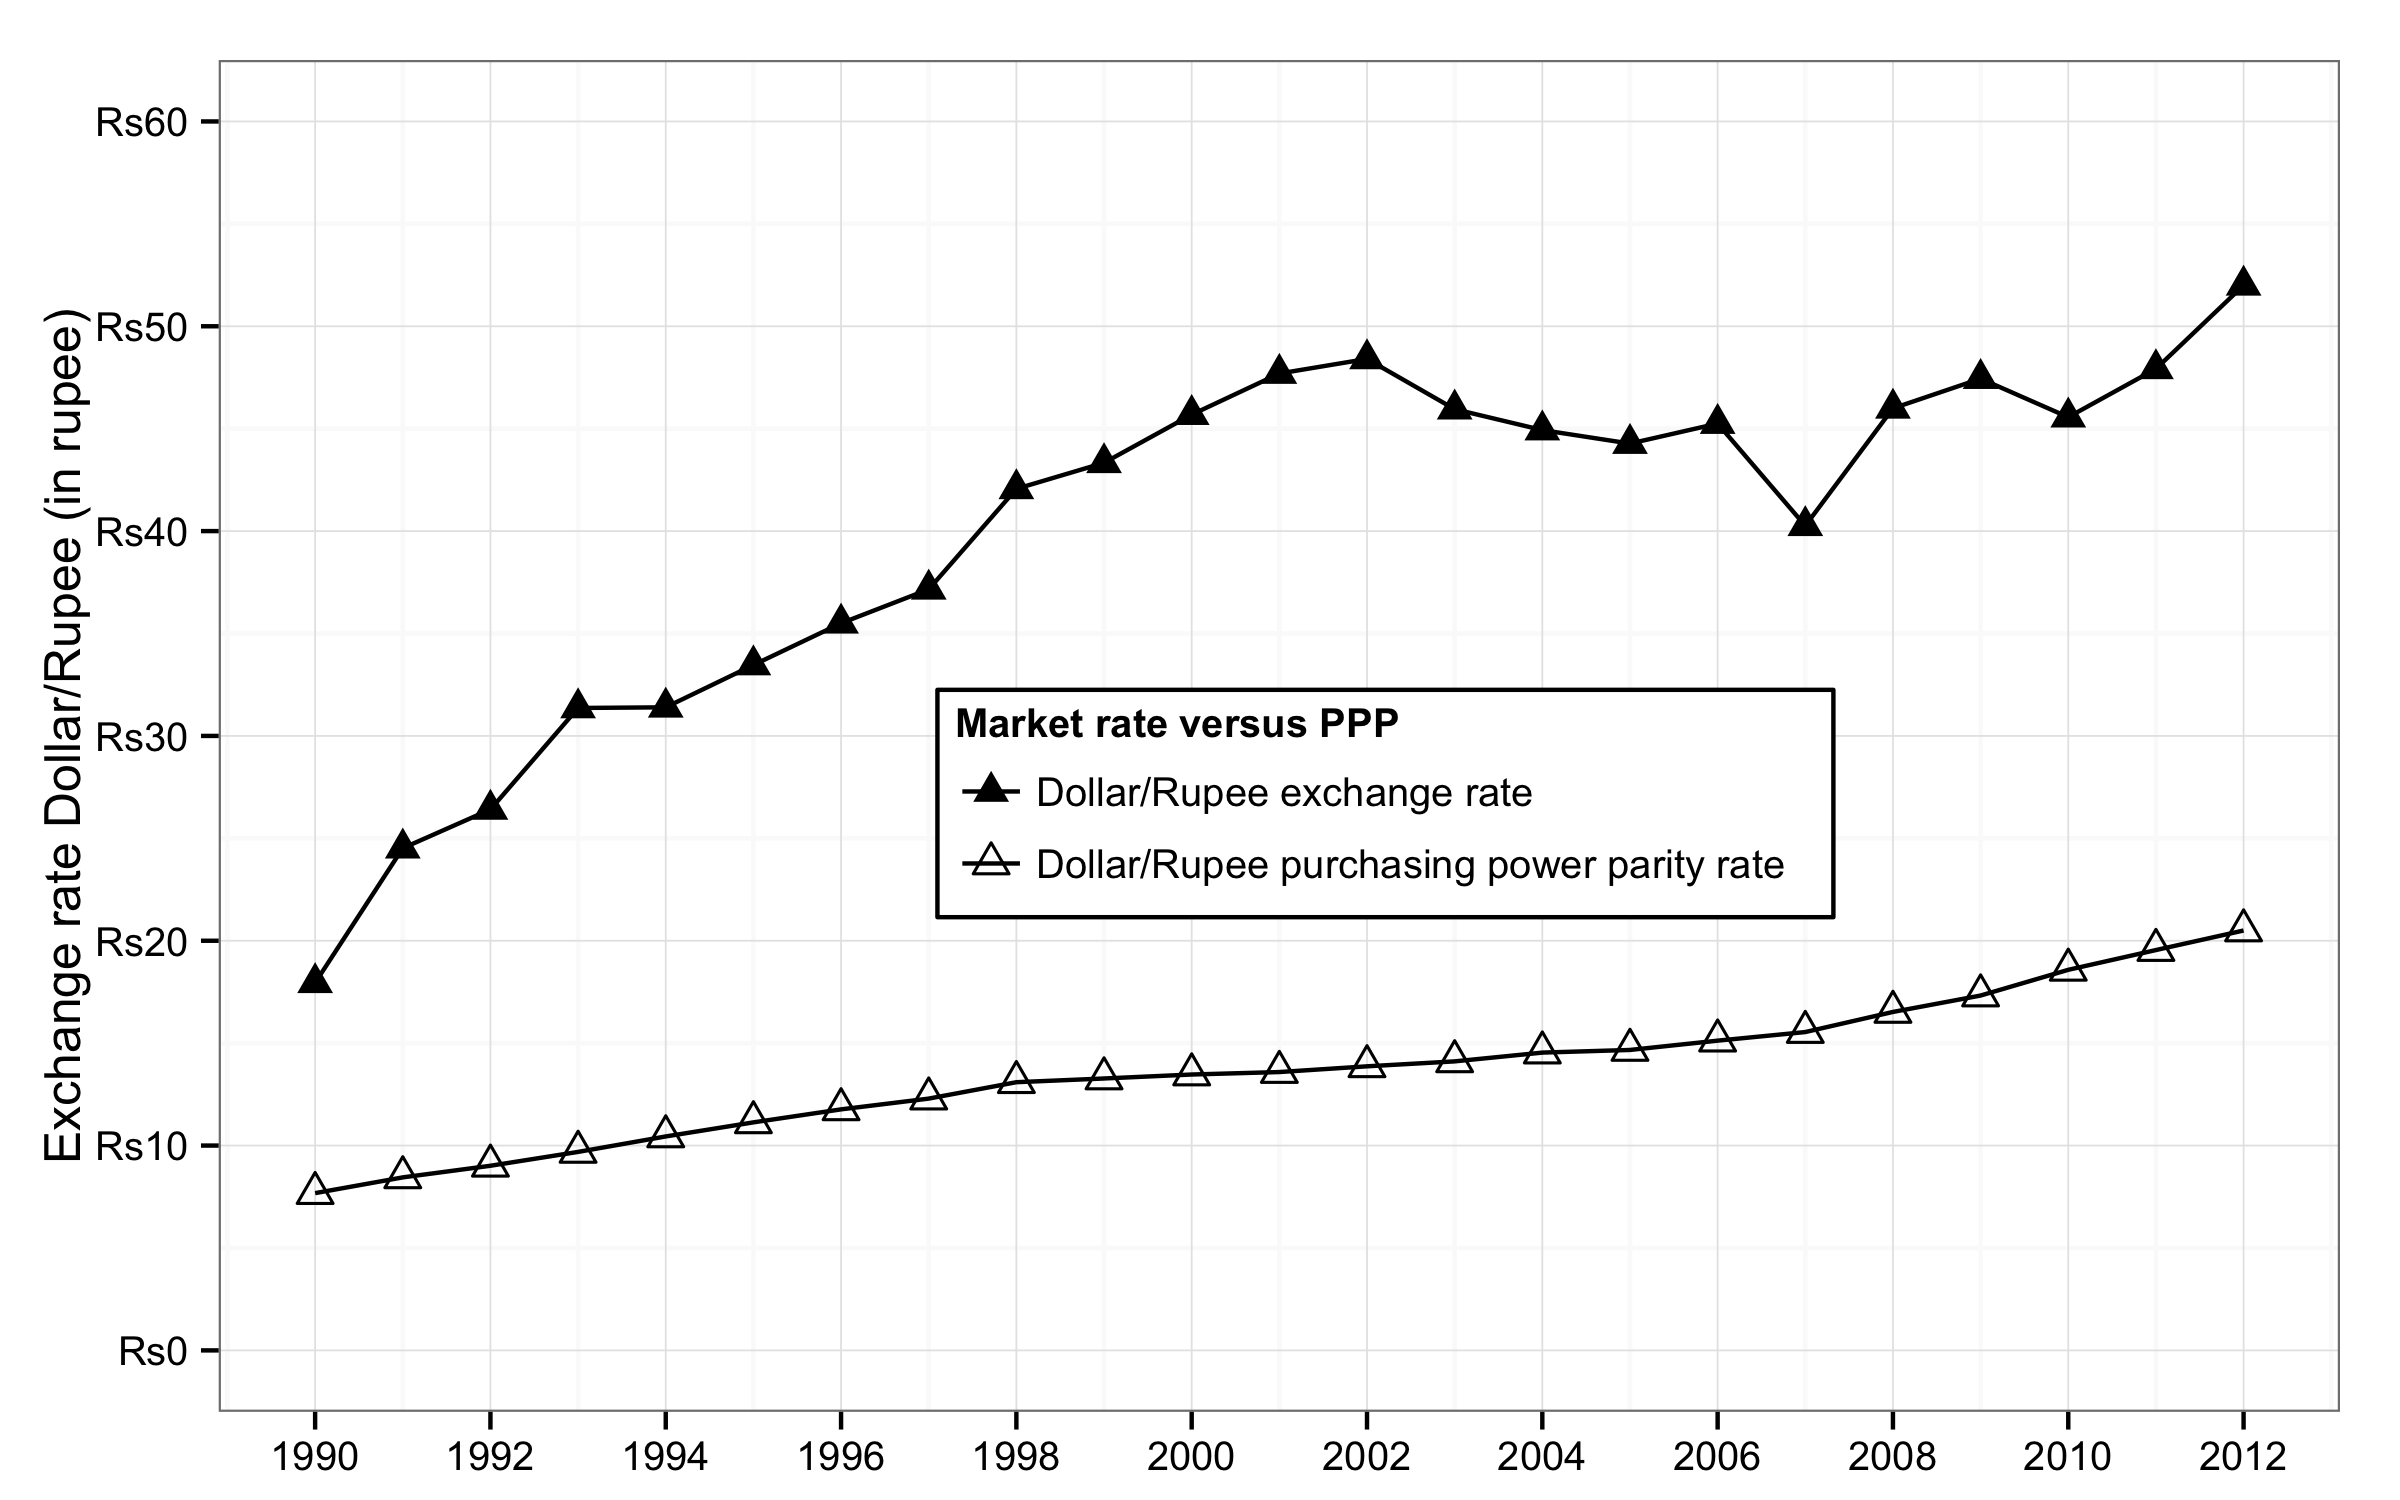
\includegraphics[width=1\linewidth]{figures/bw/Figure_S1_5b} 

}



\end{knitrout}
\caption{In 2012, 1 dollar was worth around 50 rupees according to current exchange rate, but 20 rupees in purchasing power parity.}
\end{minipage}
\end{figure}
\end{frame}
%%%%%%%%%%%%%%%%%%%% Frame Here %%%%%%%%%%%%%%%%%%%%%%%%%%%%%%%%%%%%%%%%%%%%%%%%


%%%%%%%%%%%%%%%%%%%% Frame Here %%%%%%%%%%%%%%%%%%%%%%%%%%%%%%%%%%%%%%%%%%%%%%%%
\begin{frame}[label=Figure_S1_5c,fragile]
\frametitle{Figure S1.5c. Exchange rate and purchasing power parity : dollar/yen}
\begin{figure}[t]
\begin{minipage}[b]{\textwidth}
\centering
\begin{knitrout}\footnotesize
\definecolor{shadecolor}{rgb}{0.969, 0.969, 0.969}\color{fgcolor}

{\centering 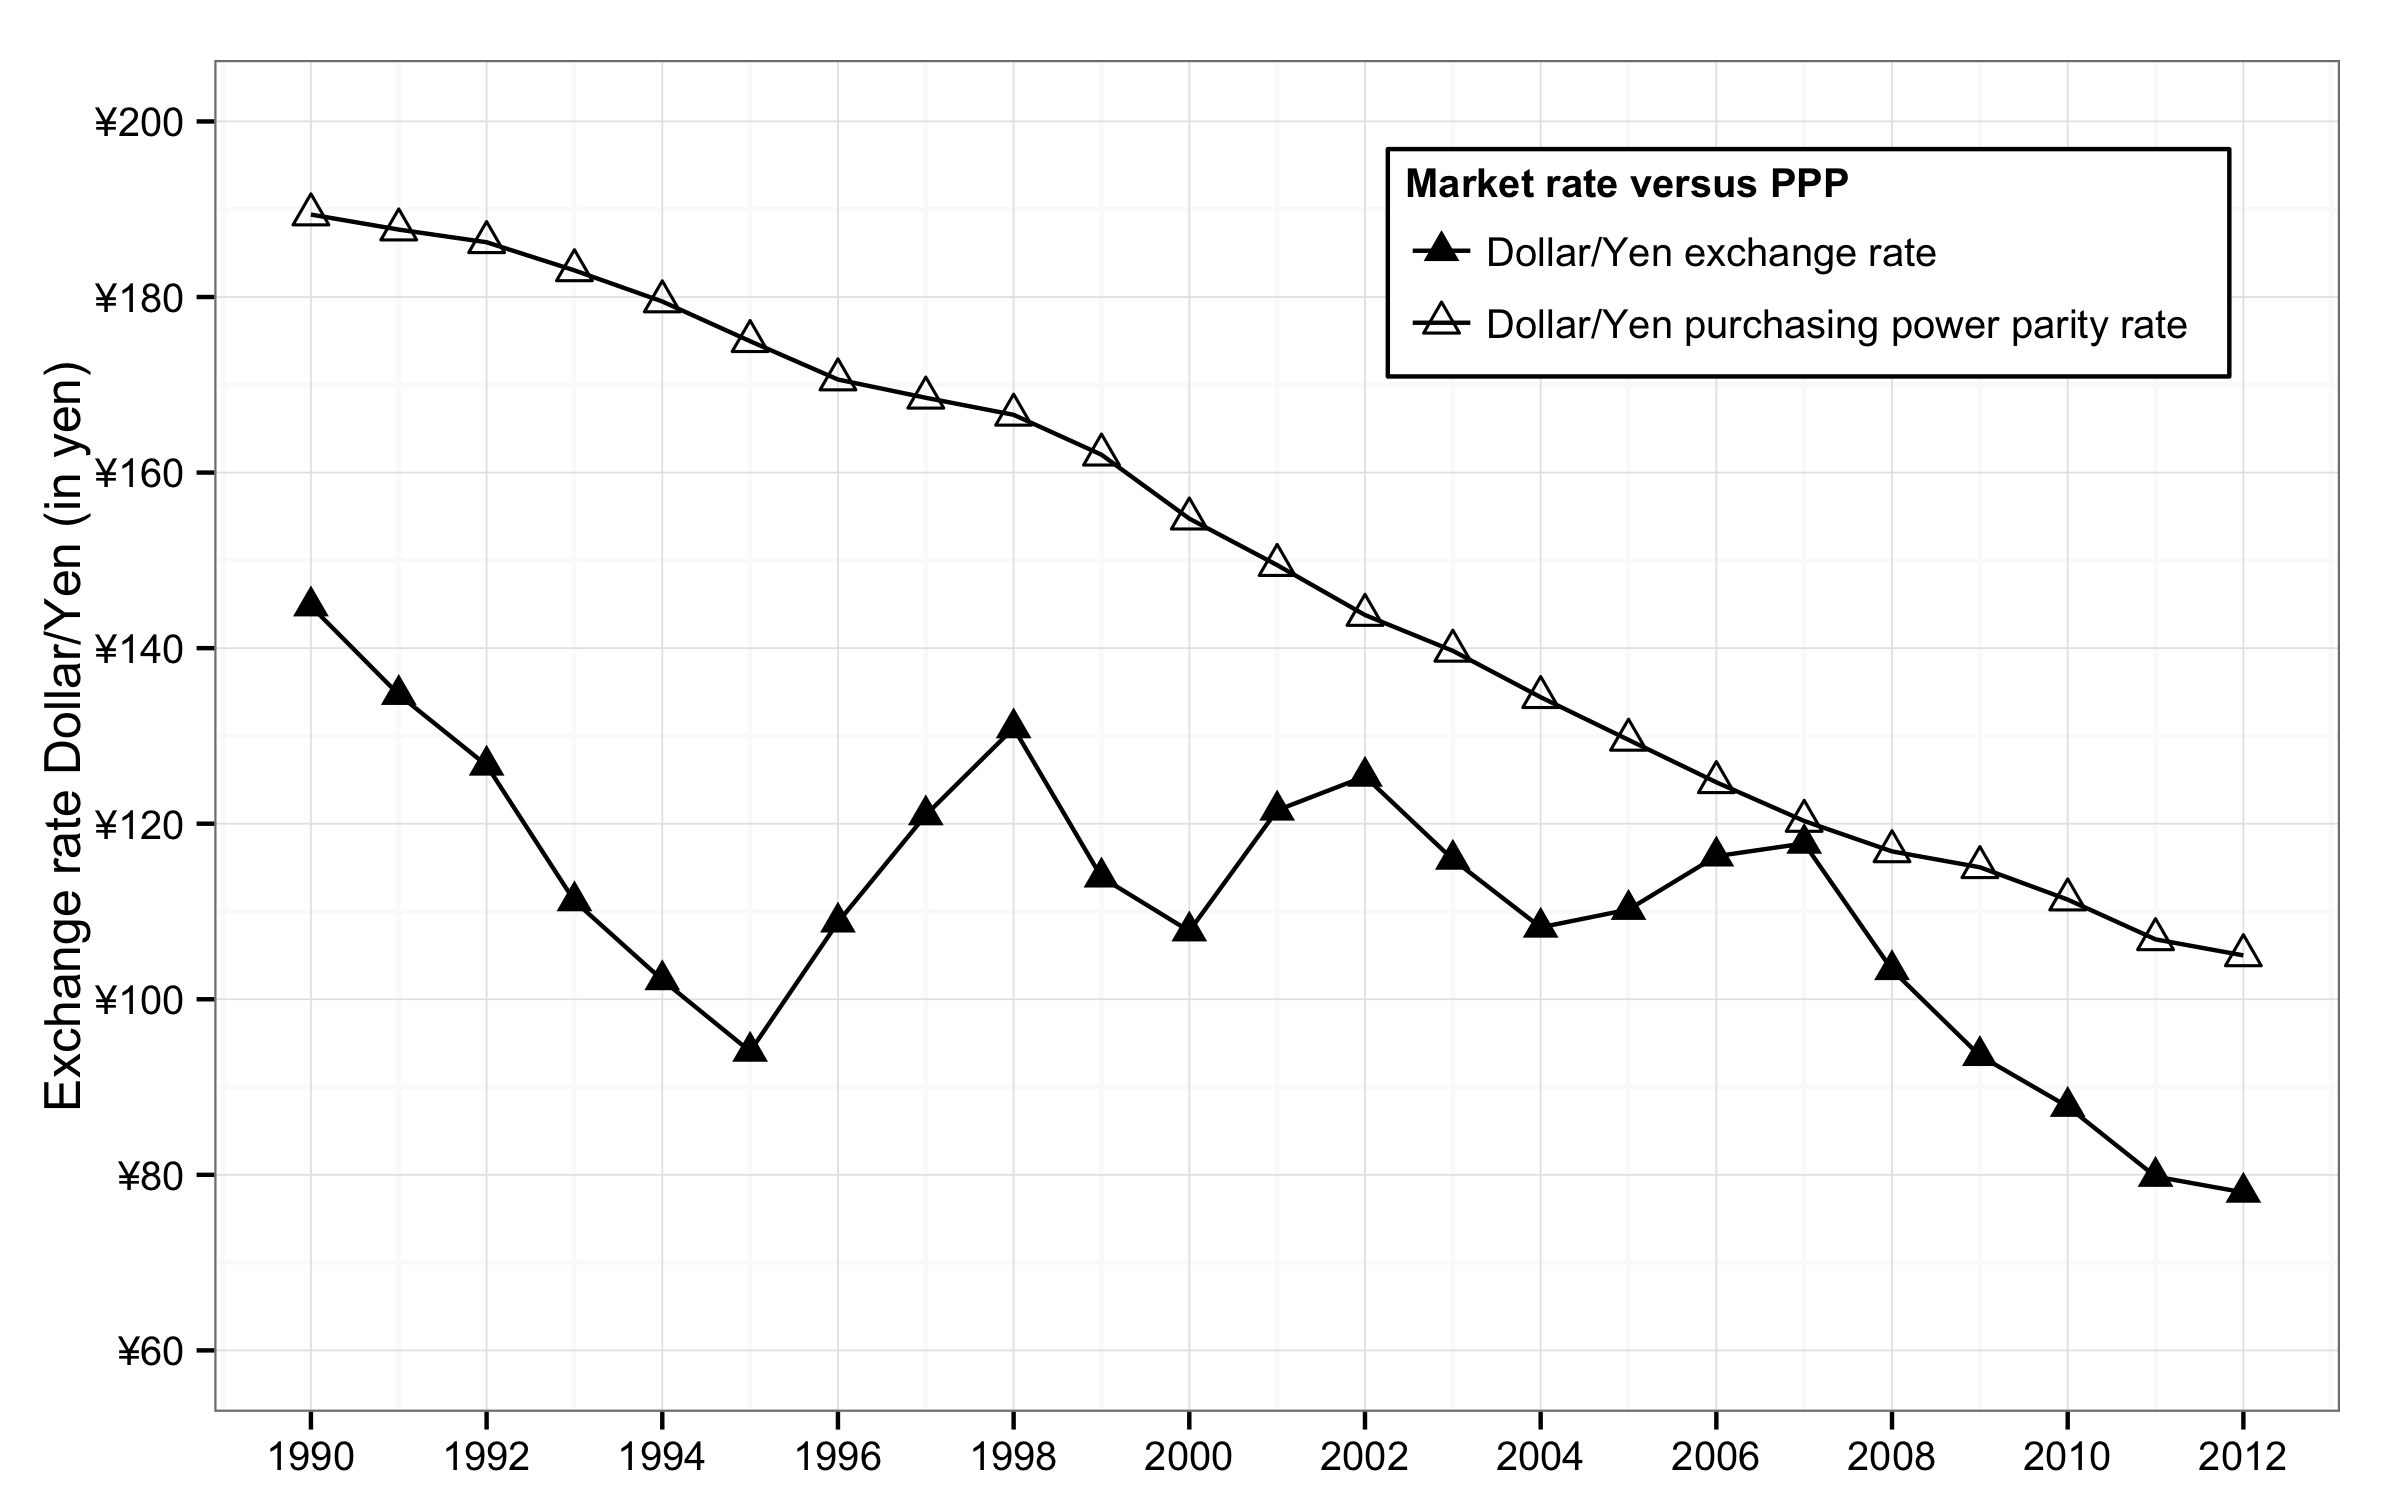
\includegraphics[width=1\linewidth]{figures/bw/Figure_S1_5c} 

}



\end{knitrout}
\caption{In 2012, 1 dollar was worth around 80 yens according to current exchange rate, but 110 yens in purchasing power parity.}
\end{minipage}
\end{figure}
\end{frame}
%%%%%%%%%%%%%%%%%%%% Frame Here %%%%%%%%%%%%%%%%%%%%%%%%%%%%%%%%%%%%%%%%%%%%%%%%


%%%%%%%%%%%%%%%%%%%% Frame Here %%%%%%%%%%%%%%%%%%%%%%%%%%%%%%%%%%%%%%%%%%%%%%%%
\begin{frame}[label=Figure_2_1]
\frametitle{Figure 2.1. The growth of world population, 1700--2012}
\begin{figure}[t]
\begin{minipage}[b]{\textwidth}
\centering
\begin{knitrout}\footnotesize
\definecolor{shadecolor}{rgb}{0.969, 0.969, 0.969}\color{fgcolor}

{\centering 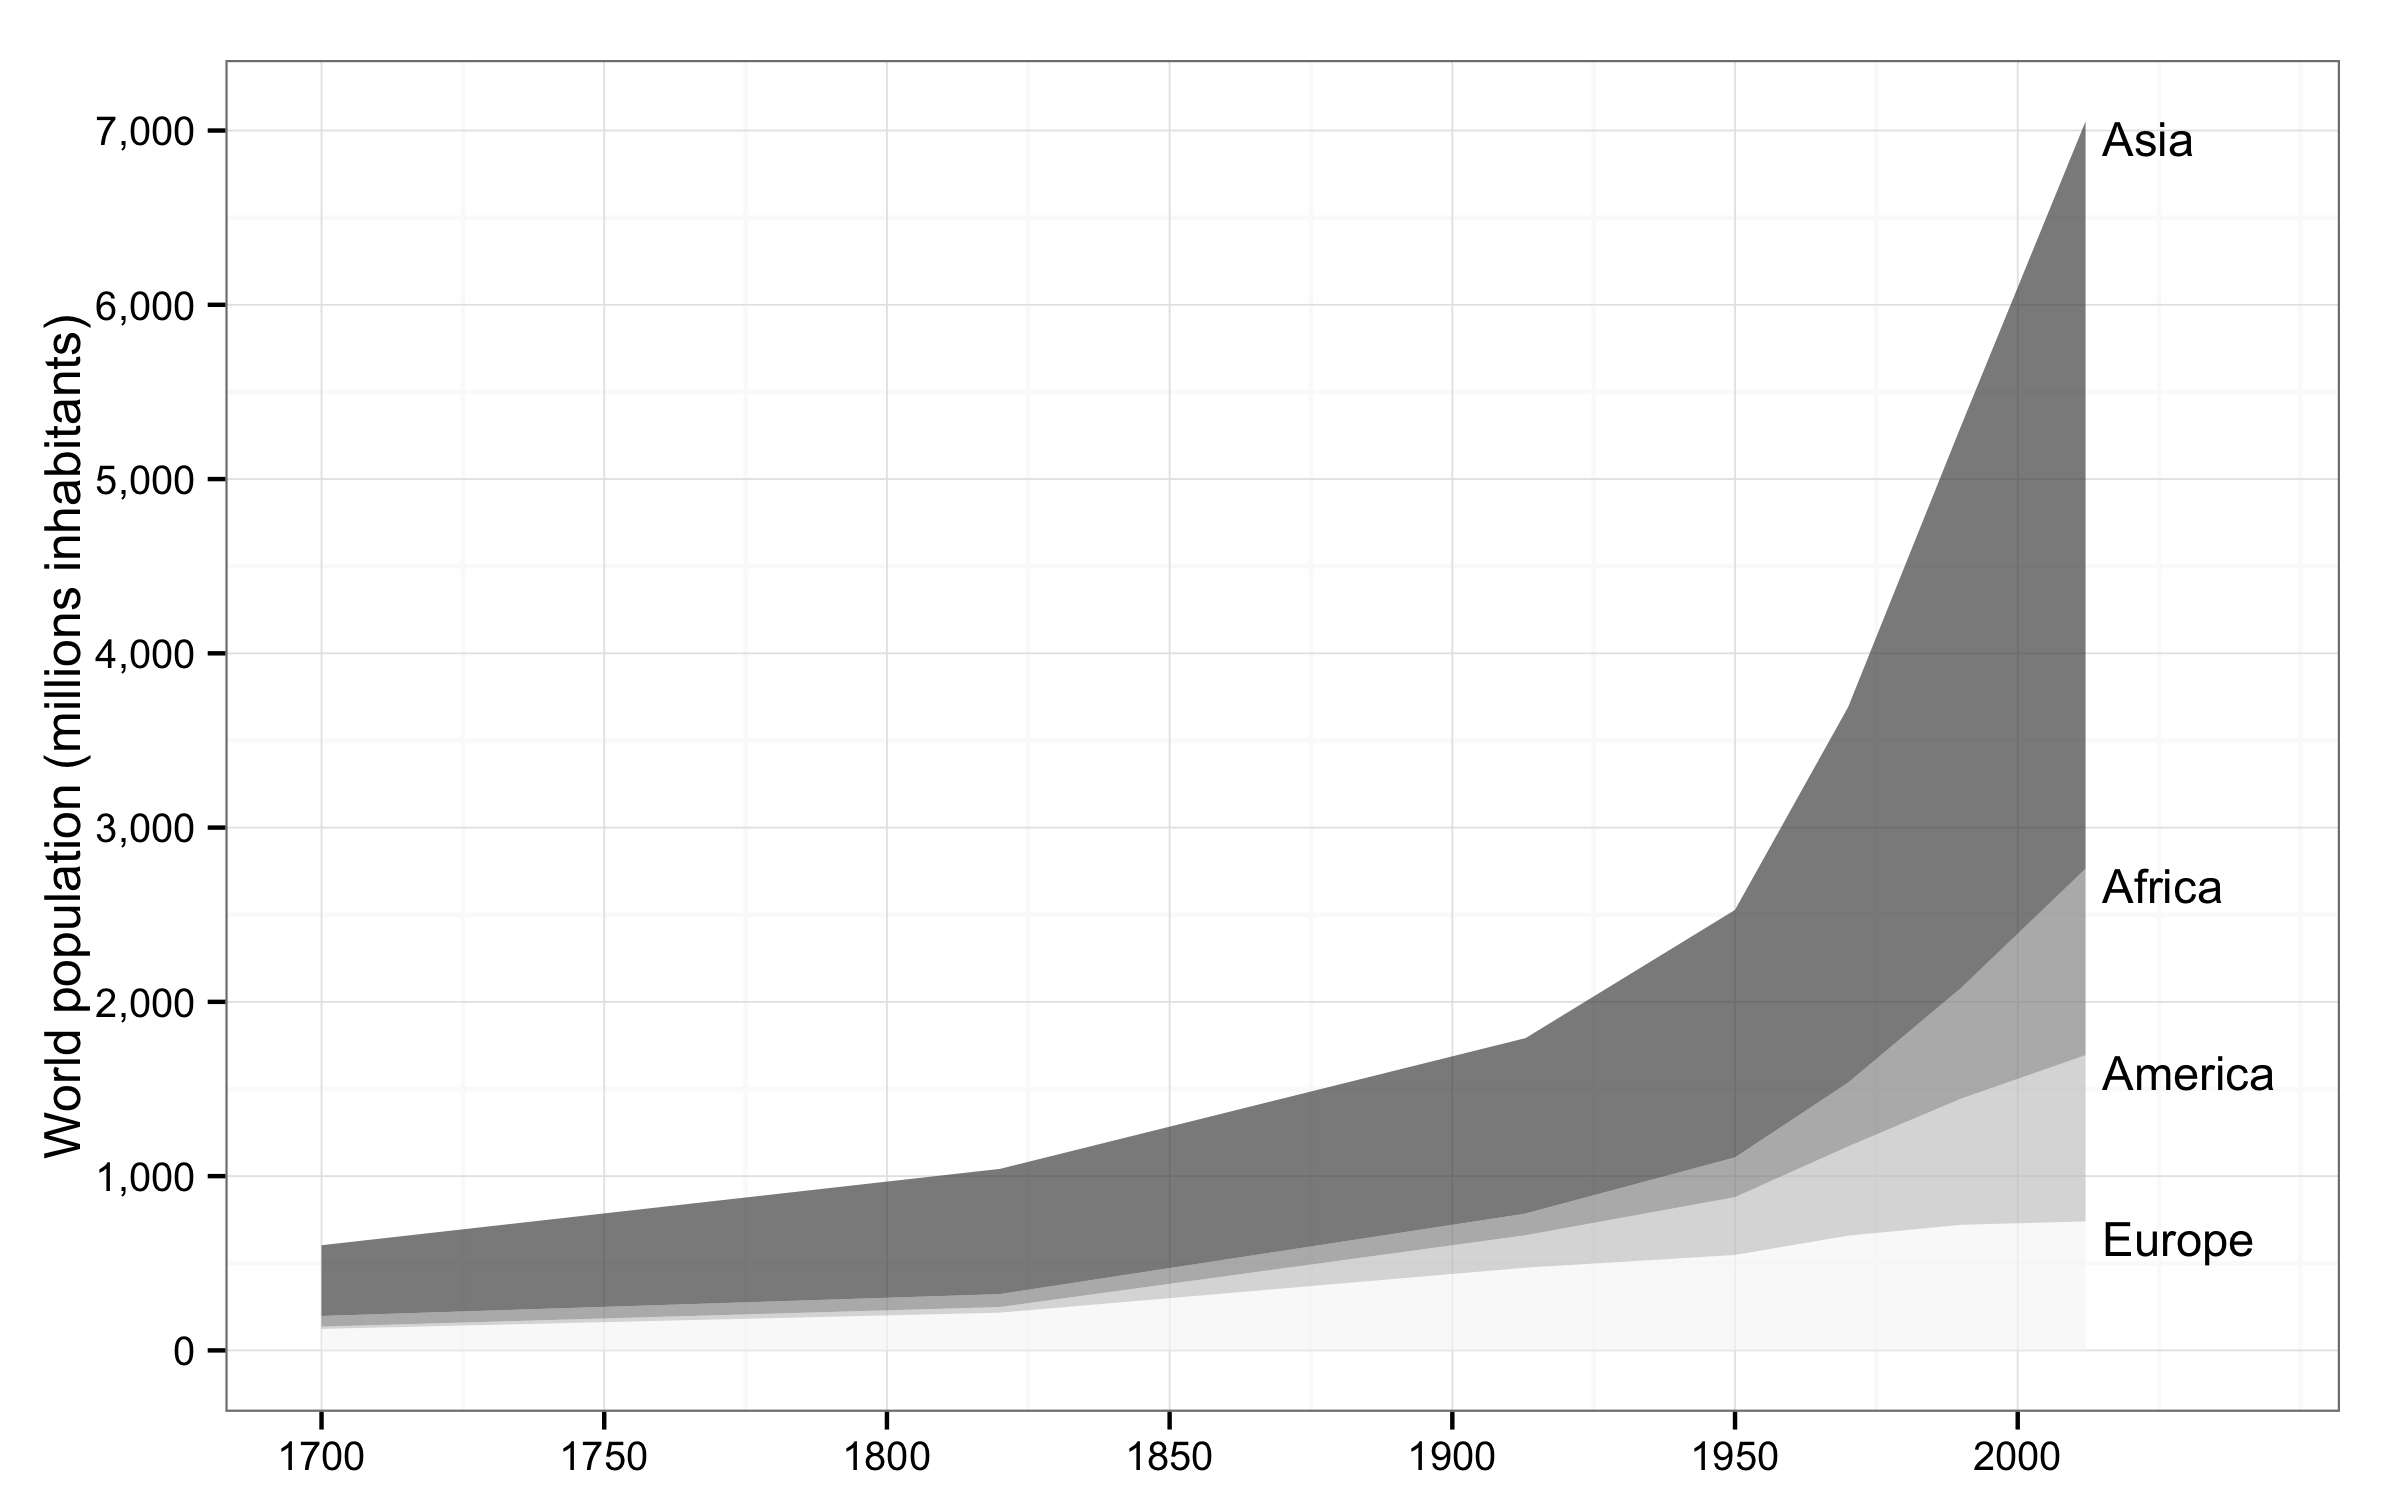
\includegraphics[width=1\linewidth]{figures/bw/Figure_2_1} 

}



\end{knitrout}
\caption{World population rose from 600 million inhabitants in 1700 to 7 billion in 2012.}
\end{minipage}
\end{figure}
\end{frame}
%%%%%%%%%%%%%%%%%%%% Frame Here %%%%%%%%%%%%%%%%%%%%%%%%%%%%%%%%%%%%%%%%%%%%%%%%


%%%%%%%%%%%%%%%%%%%% Frame Here %%%%%%%%%%%%%%%%%%%%%%%%%%%%%%%%%%%%%%%%%%%%%%%%
\begin{frame}[label=Figure_2_1b]
\frametitle{Figure 2.1. The growth of world population, 1700--2012}
\begin{figure}[t]
\begin{minipage}[b]{\textwidth}
\centering
\begin{knitrout}\footnotesize
\definecolor{shadecolor}{rgb}{0.969, 0.969, 0.969}\color{fgcolor}

{\centering 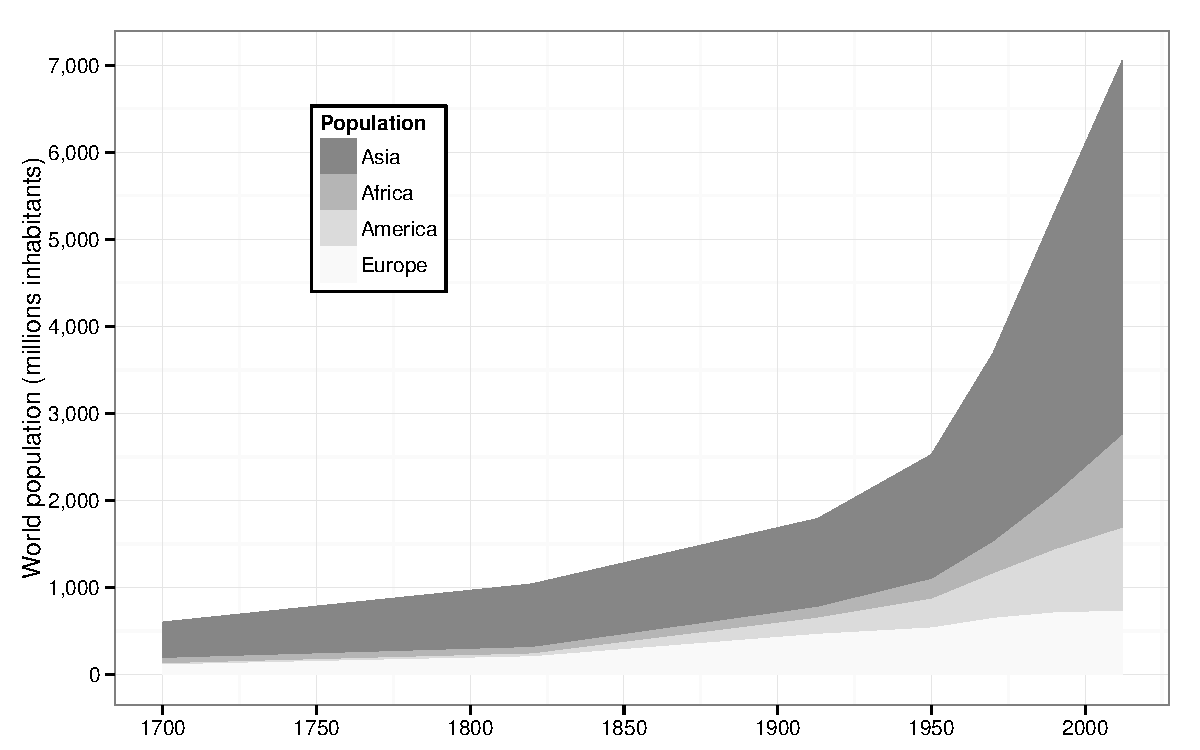
\includegraphics[width=1\linewidth]{figures/bw/Figure_2_1b} 

}



\end{knitrout}
\caption{World population rose from 600 million inhabitants in 1700 to 7 billion in 2012.}
\end{minipage}
\end{figure}
\end{frame}
%%%%%%%%%%%%%%%%%%%% Frame Here %%%%%%%%%%%%%%%%%%%%%%%%%%%%%%%%%%%%%%%%%%%%%%%%


%%%%%%%%%%%%%%%%%%%% Frame Here %%%%%%%%%%%%%%%%%%%%%%%%%%%%%%%%%%%%%%%%%%%%%%%%
\begin{frame}[label=Figure_2_2S]
\frametitle{Figure 2.2S. The growth rate of population from Antiquity to 2100}
\begin{figure}[t]
\begin{minipage}[b]{\textwidth}
\centering
\begin{knitrout}\footnotesize
\definecolor{shadecolor}{rgb}{0.969, 0.969, 0.969}\color{fgcolor}

{\centering 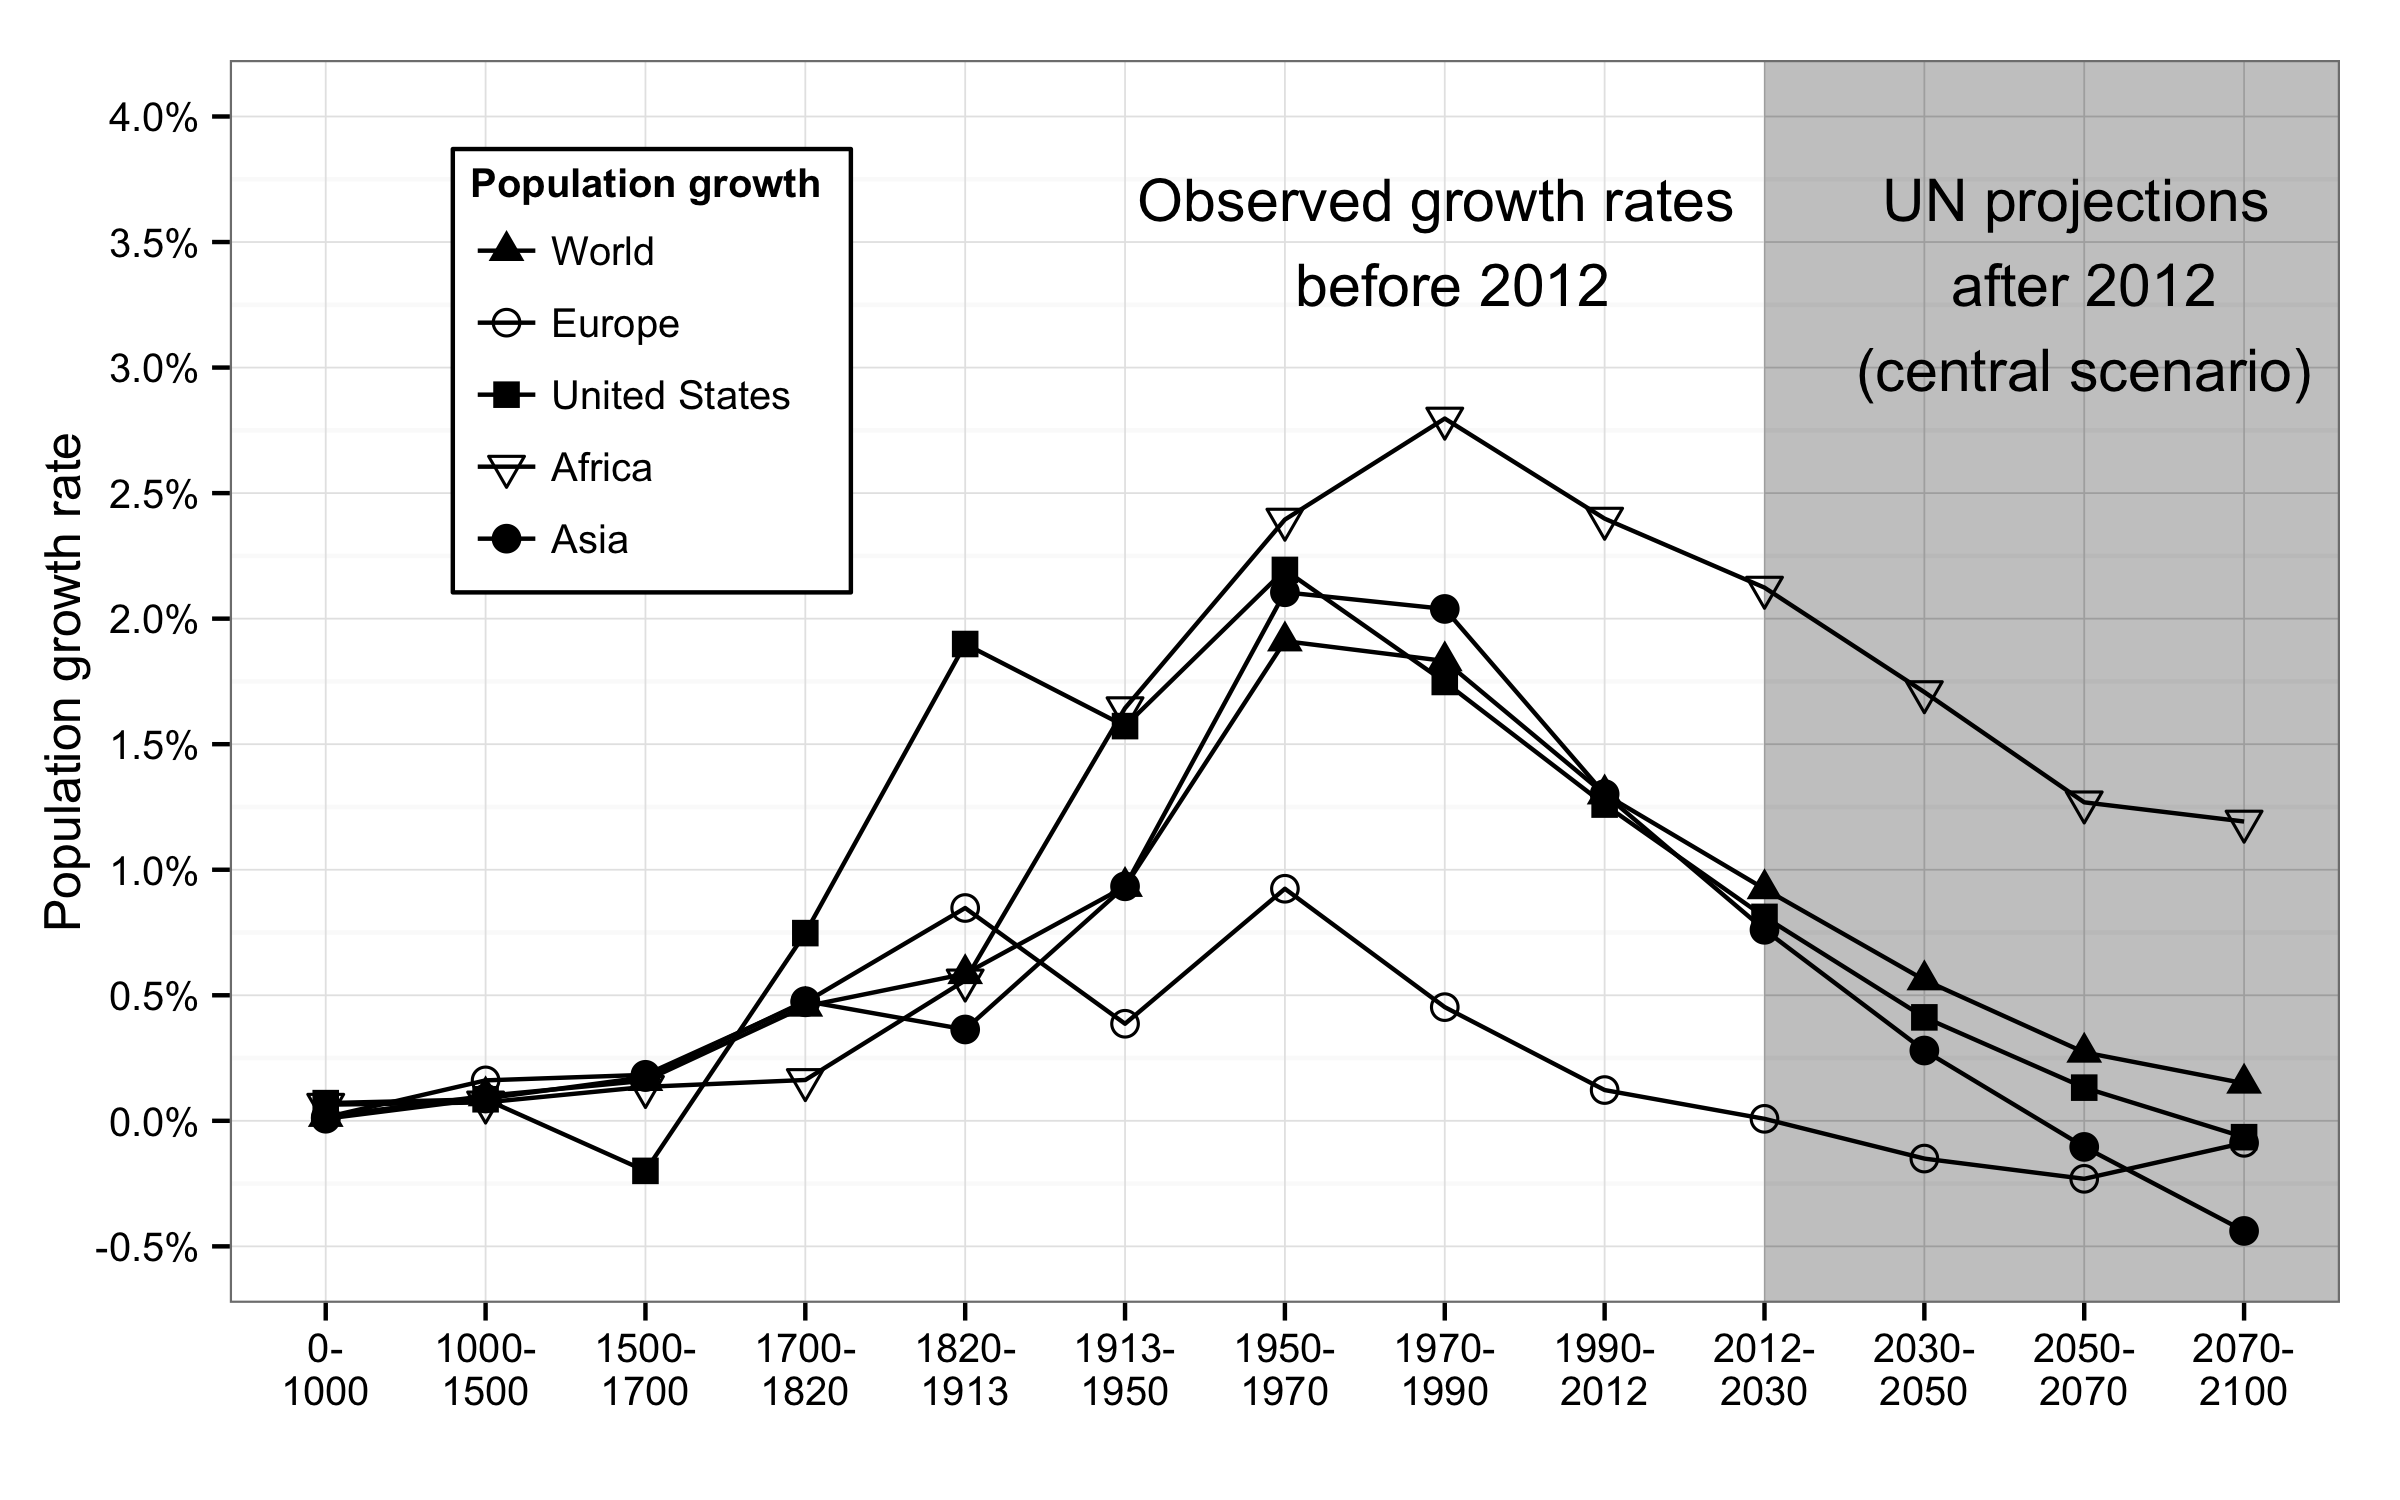
\includegraphics[width=1\linewidth]{figures/bw/Figure_2_2S} 

}



\end{knitrout}
\caption{The growth rate of world population was above 1 percent per year from 1950 to 2012 and should return toward 0 percent by the end of the twenty-first century.}
\end{minipage}
\end{figure}
\end{frame}
%%%%%%%%%%%%%%%%%%%% Frame Here %%%%%%%%%%%%%%%%%%%%%%%%%%%%%%%%%%%%%%%%%%%%%%%%


%%%%%%%%%%%%%%%%%%%% Frame Here %%%%%%%%%%%%%%%%%%%%%%%%%%%%%%%%%%%%%%%%%%%%%%%%
\begin{frame}[label=Figure_2_2]
\frametitle{Figure 2.2. The growth rate of world population from Antiquity to 2100}
\begin{figure}[t]
\begin{minipage}[b]{\textwidth}
\centering
\begin{knitrout}\footnotesize
\definecolor{shadecolor}{rgb}{0.969, 0.969, 0.969}\color{fgcolor}

{\centering 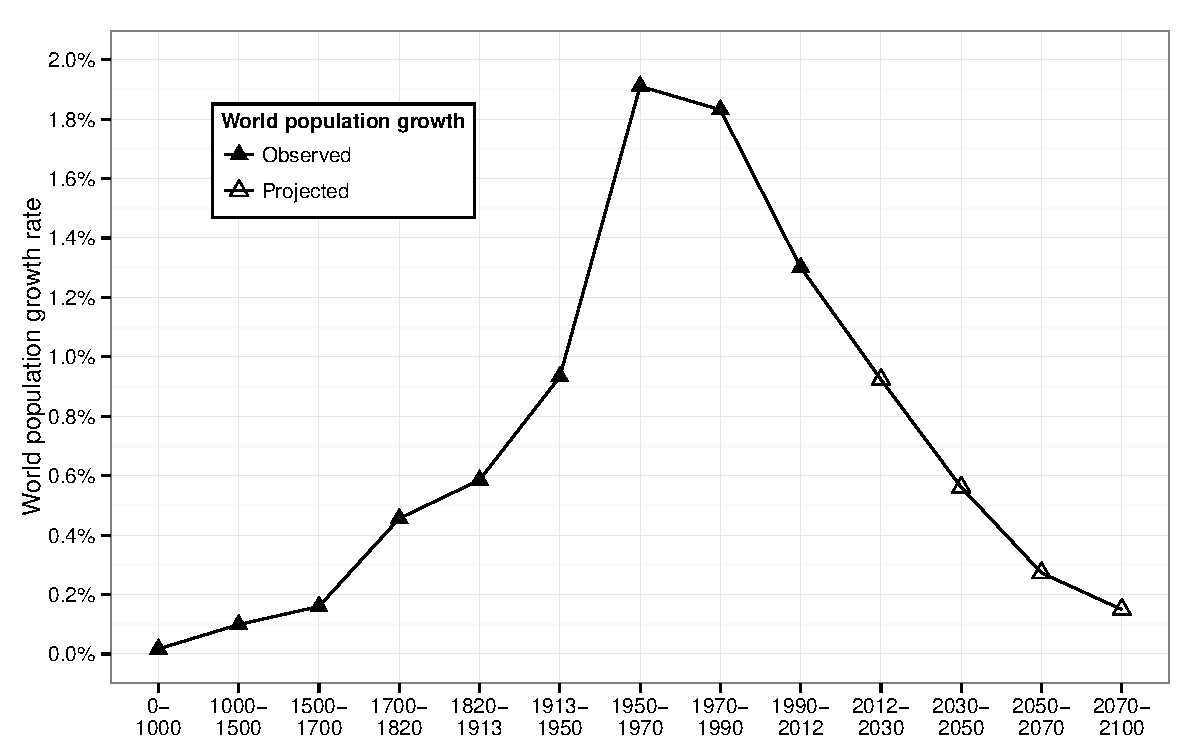
\includegraphics[width=1\linewidth]{figures/bw/Figure_2_2} 

}



\end{knitrout}
\caption{The growth rate of world population was above 1 percent per year from 1950 to 2012 and should return toward 0 percent by the end of the twenty-first century.}
\end{minipage}
\end{figure}
\end{frame}
%%%%%%%%%%%%%%%%%%%% Frame Here %%%%%%%%%%%%%%%%%%%%%%%%%%%%%%%%%%%%%%%%%%%%%%%%


%%%%%%%%%%%%%%%%%%%% Frame Here %%%%%%%%%%%%%%%%%%%%%%%%%%%%%%%%%%%%%%%%%%%%%%%%
\begin{frame}[label=Figure_2_3]
\frametitle{Figure 2.3. The growth rate of per capita output since the Industrial Revolution}
\begin{figure}[t]
\begin{minipage}[b]{\textwidth}
\centering
\begin{knitrout}\footnotesize
\definecolor{shadecolor}{rgb}{0.969, 0.969, 0.969}\color{fgcolor}

{\centering 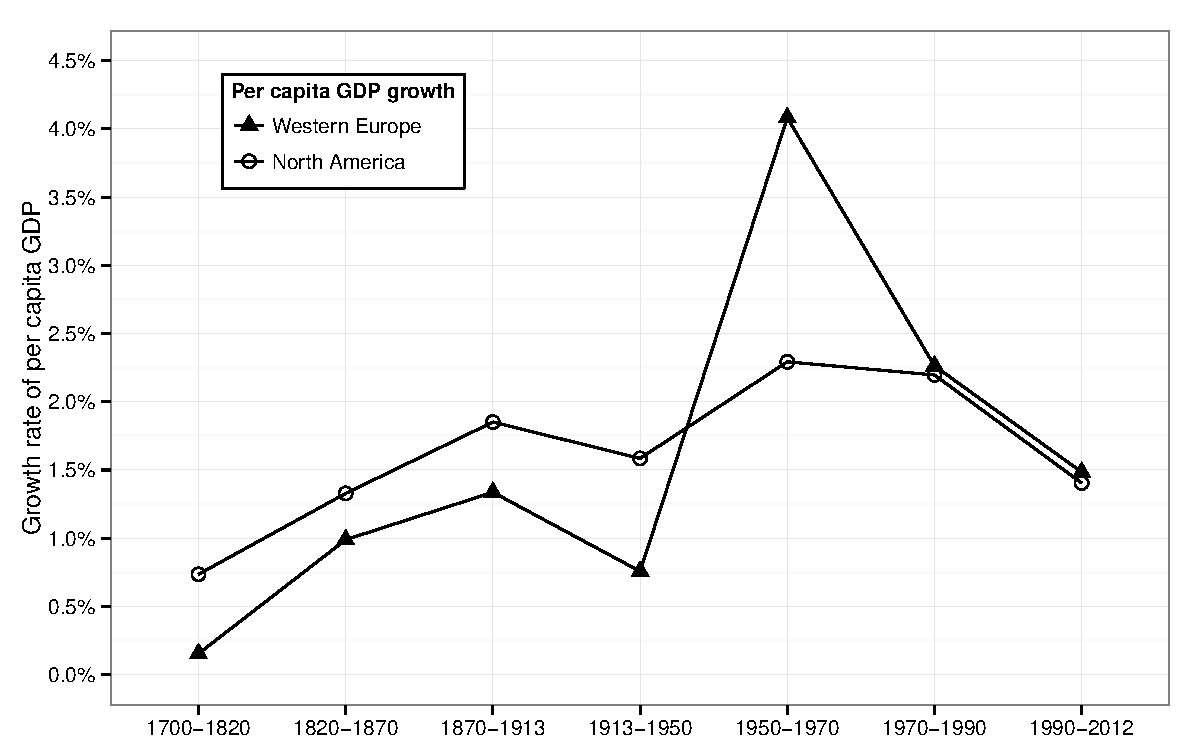
\includegraphics[width=1\linewidth]{figures/bw/Figure_2_3} 

}



\end{knitrout}
\caption{The growth rate of per capita output surpassed 4 percent per year in Europe between 1950 and 1970, before returning to American levels.}
\end{minipage}
\end{figure}
\end{frame}
%%%%%%%%%%%%%%%%%%%% Frame Here %%%%%%%%%%%%%%%%%%%%%%%%%%%%%%%%%%%%%%%%%%%%%%%%


%%%%%%%%%%%%%%%%%%%% Frame Here %%%%%%%%%%%%%%%%%%%%%%%%%%%%%%%%%%%%%%%%%%%%%%%%
\begin{frame}[label=Figure_2_4]
\frametitle{Figure 2.4. The growth rate of world per capita output from Antiquity to 2100}
\begin{figure}[t]
\begin{minipage}[b]{\textwidth}
\centering
\begin{knitrout}\footnotesize
\definecolor{shadecolor}{rgb}{0.969, 0.969, 0.969}\color{fgcolor}

{\centering 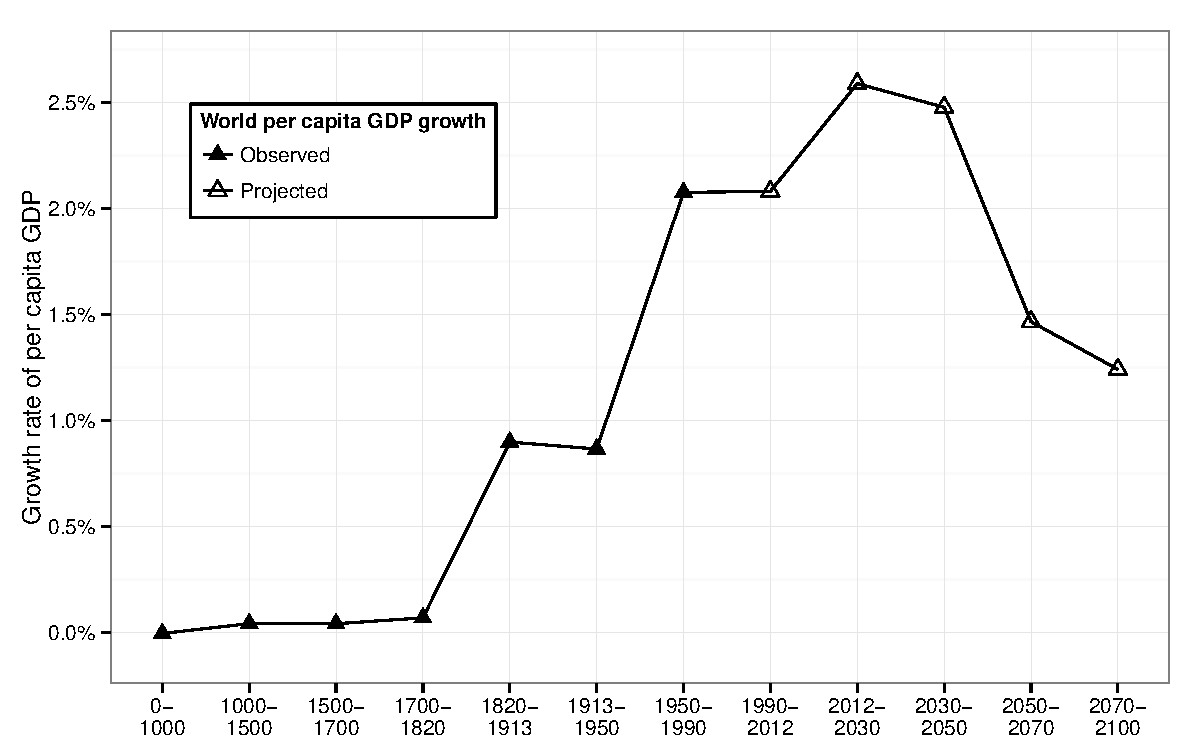
\includegraphics[width=1\linewidth]{figures/bw/Figure_2_4} 

}



\end{knitrout}
\caption{The growth rate of per capita output surpassed 2 percent from 1950 to 2012. If the convergence process goes on, it will surpass 2.5 percent from 2012 to 2050, and then will drop below 1.5 percent.}
\end{minipage}
\end{figure}
\end{frame}
%%%%%%%%%%%%%%%%%%%% Frame Here %%%%%%%%%%%%%%%%%%%%%%%%%%%%%%%%%%%%%%%%%%%%%%%%


%%%%%%%%%%%%%%%%%%%% Frame Here %%%%%%%%%%%%%%%%%%%%%%%%%%%%%%%%%%%%%%%%%%%%%%%%
\begin{frame}[label=Figure_2_5]
\frametitle{Figure 2.5. The growth rate of world output from Antiquity to 2100}
\begin{figure}[t]
\begin{minipage}[b]{\textwidth}
\centering
\begin{knitrout}\footnotesize
\definecolor{shadecolor}{rgb}{0.969, 0.969, 0.969}\color{fgcolor}

{\centering 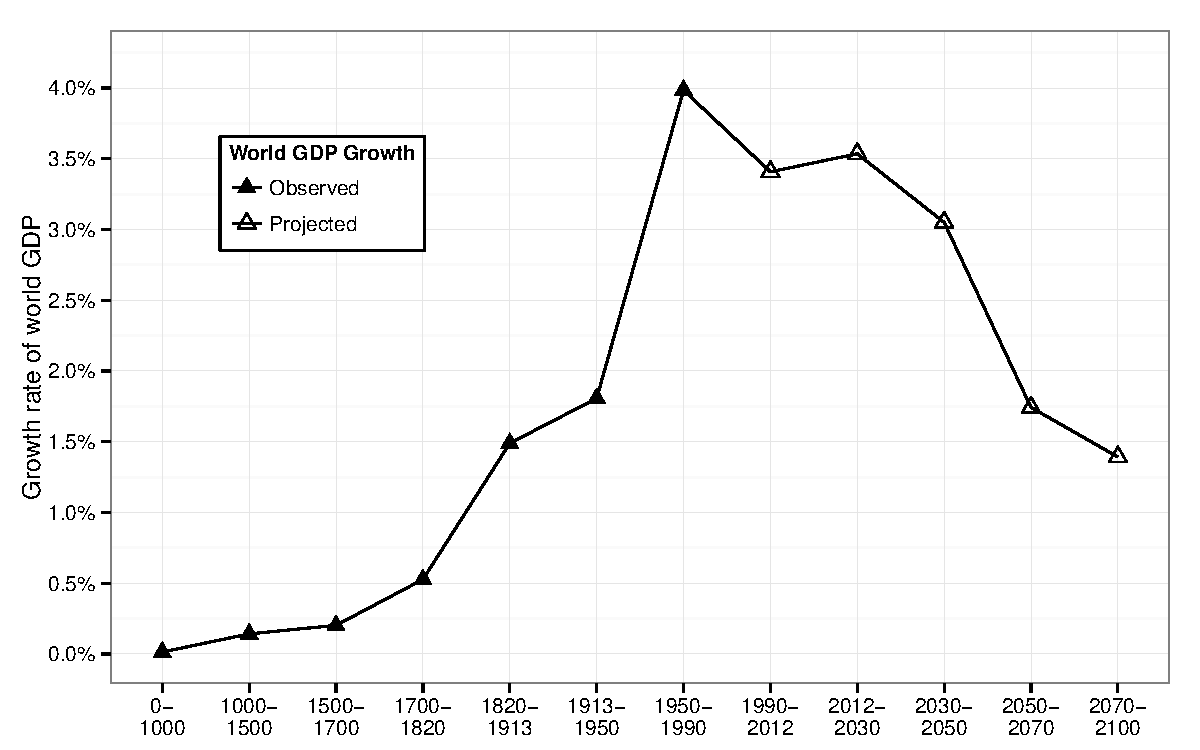
\includegraphics[width=1\linewidth]{figures/bw/Figure_2_5} 

}



\end{knitrout}
\caption{The growth rate of world output surpassed 4 percent from 1950 to 1990. If the convergence process goes on, it will drop below 2 percent by 2050.}
\end{minipage}
\end{figure}
\end{frame}
%%%%%%%%%%%%%%%%%%%% Frame Here %%%%%%%%%%%%%%%%%%%%%%%%%%%%%%%%%%%%%%%%%%%%%%%%


%%%%%%%%%%%%%%%%%%%% Frame Here %%%%%%%%%%%%%%%%%%%%%%%%%%%%%%%%%%%%%%%%%%%%%%%%
\begin{frame}[label=Figure_2_6,fragile]
\frametitle{Figure 2.6. Inflation since the Industrial Revolution}
\begin{figure}[t]
\begin{minipage}[b]{\textwidth}
\centering
\begin{knitrout}\footnotesize
\definecolor{shadecolor}{rgb}{0.969, 0.969, 0.969}\color{fgcolor}

{\centering 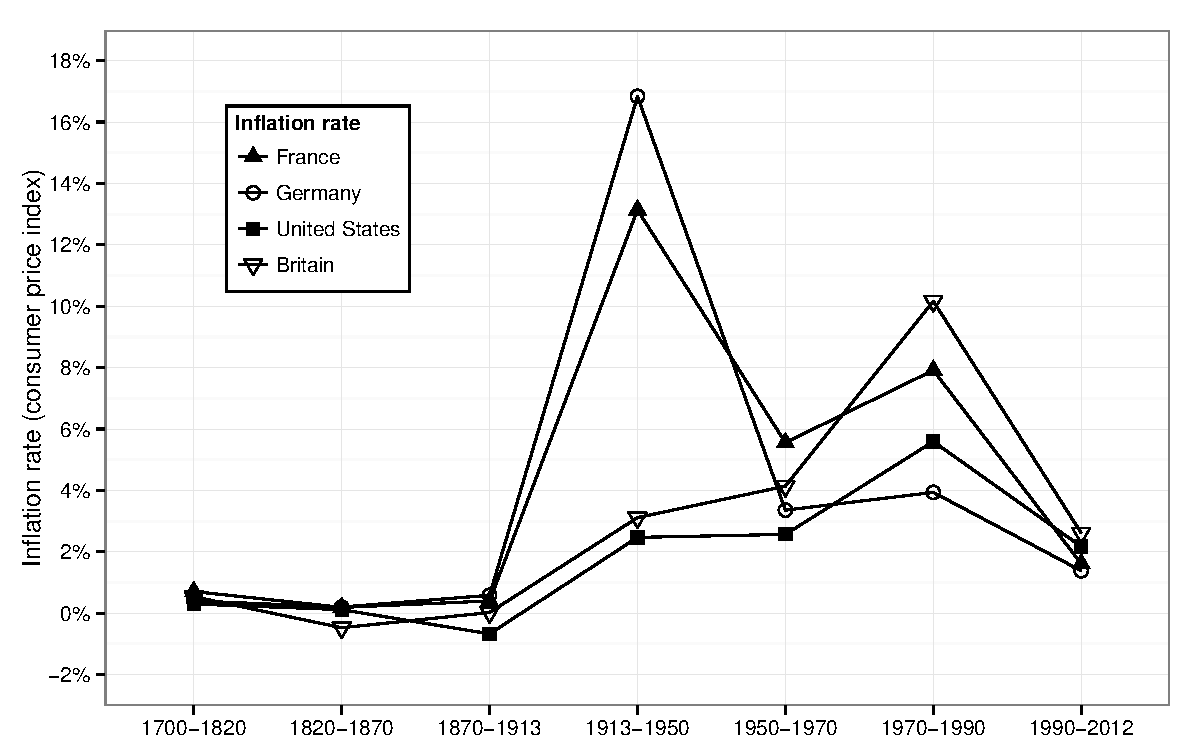
\includegraphics[width=1\linewidth]{figures/bw/Figure_2_6} 

}



\end{knitrout}
\caption{Inflation in the rich countries was zero in the eighteenth and nineteenth centuries, high in the twentieth century, and roughly 2 percent a year since 1990.}
\end{minipage}
\end{figure}
\end{frame}
%%%%%%%%%%%%%%%%%%%% Frame Here %%%%%%%%%%%%%%%%%%%%%%%%%%%%%%%%%%%%%%%%%%%%%%%%


%%%%%%%%%%%%%%%%%%%% Frame Here %%%%%%%%%%%%%%%%%%%%%%%%%%%%%%%%%%%%%%%%%%%%%%%%
\begin{frame}[label=Figure_3_1]
\frametitle{Figure 3.1. Capital in Britain, 1700--2010}
\begin{figure}[t]
\begin{minipage}[b]{\textwidth}
\centering
\begin{knitrout}\footnotesize
\definecolor{shadecolor}{rgb}{0.969, 0.969, 0.969}\color{fgcolor}

{\centering 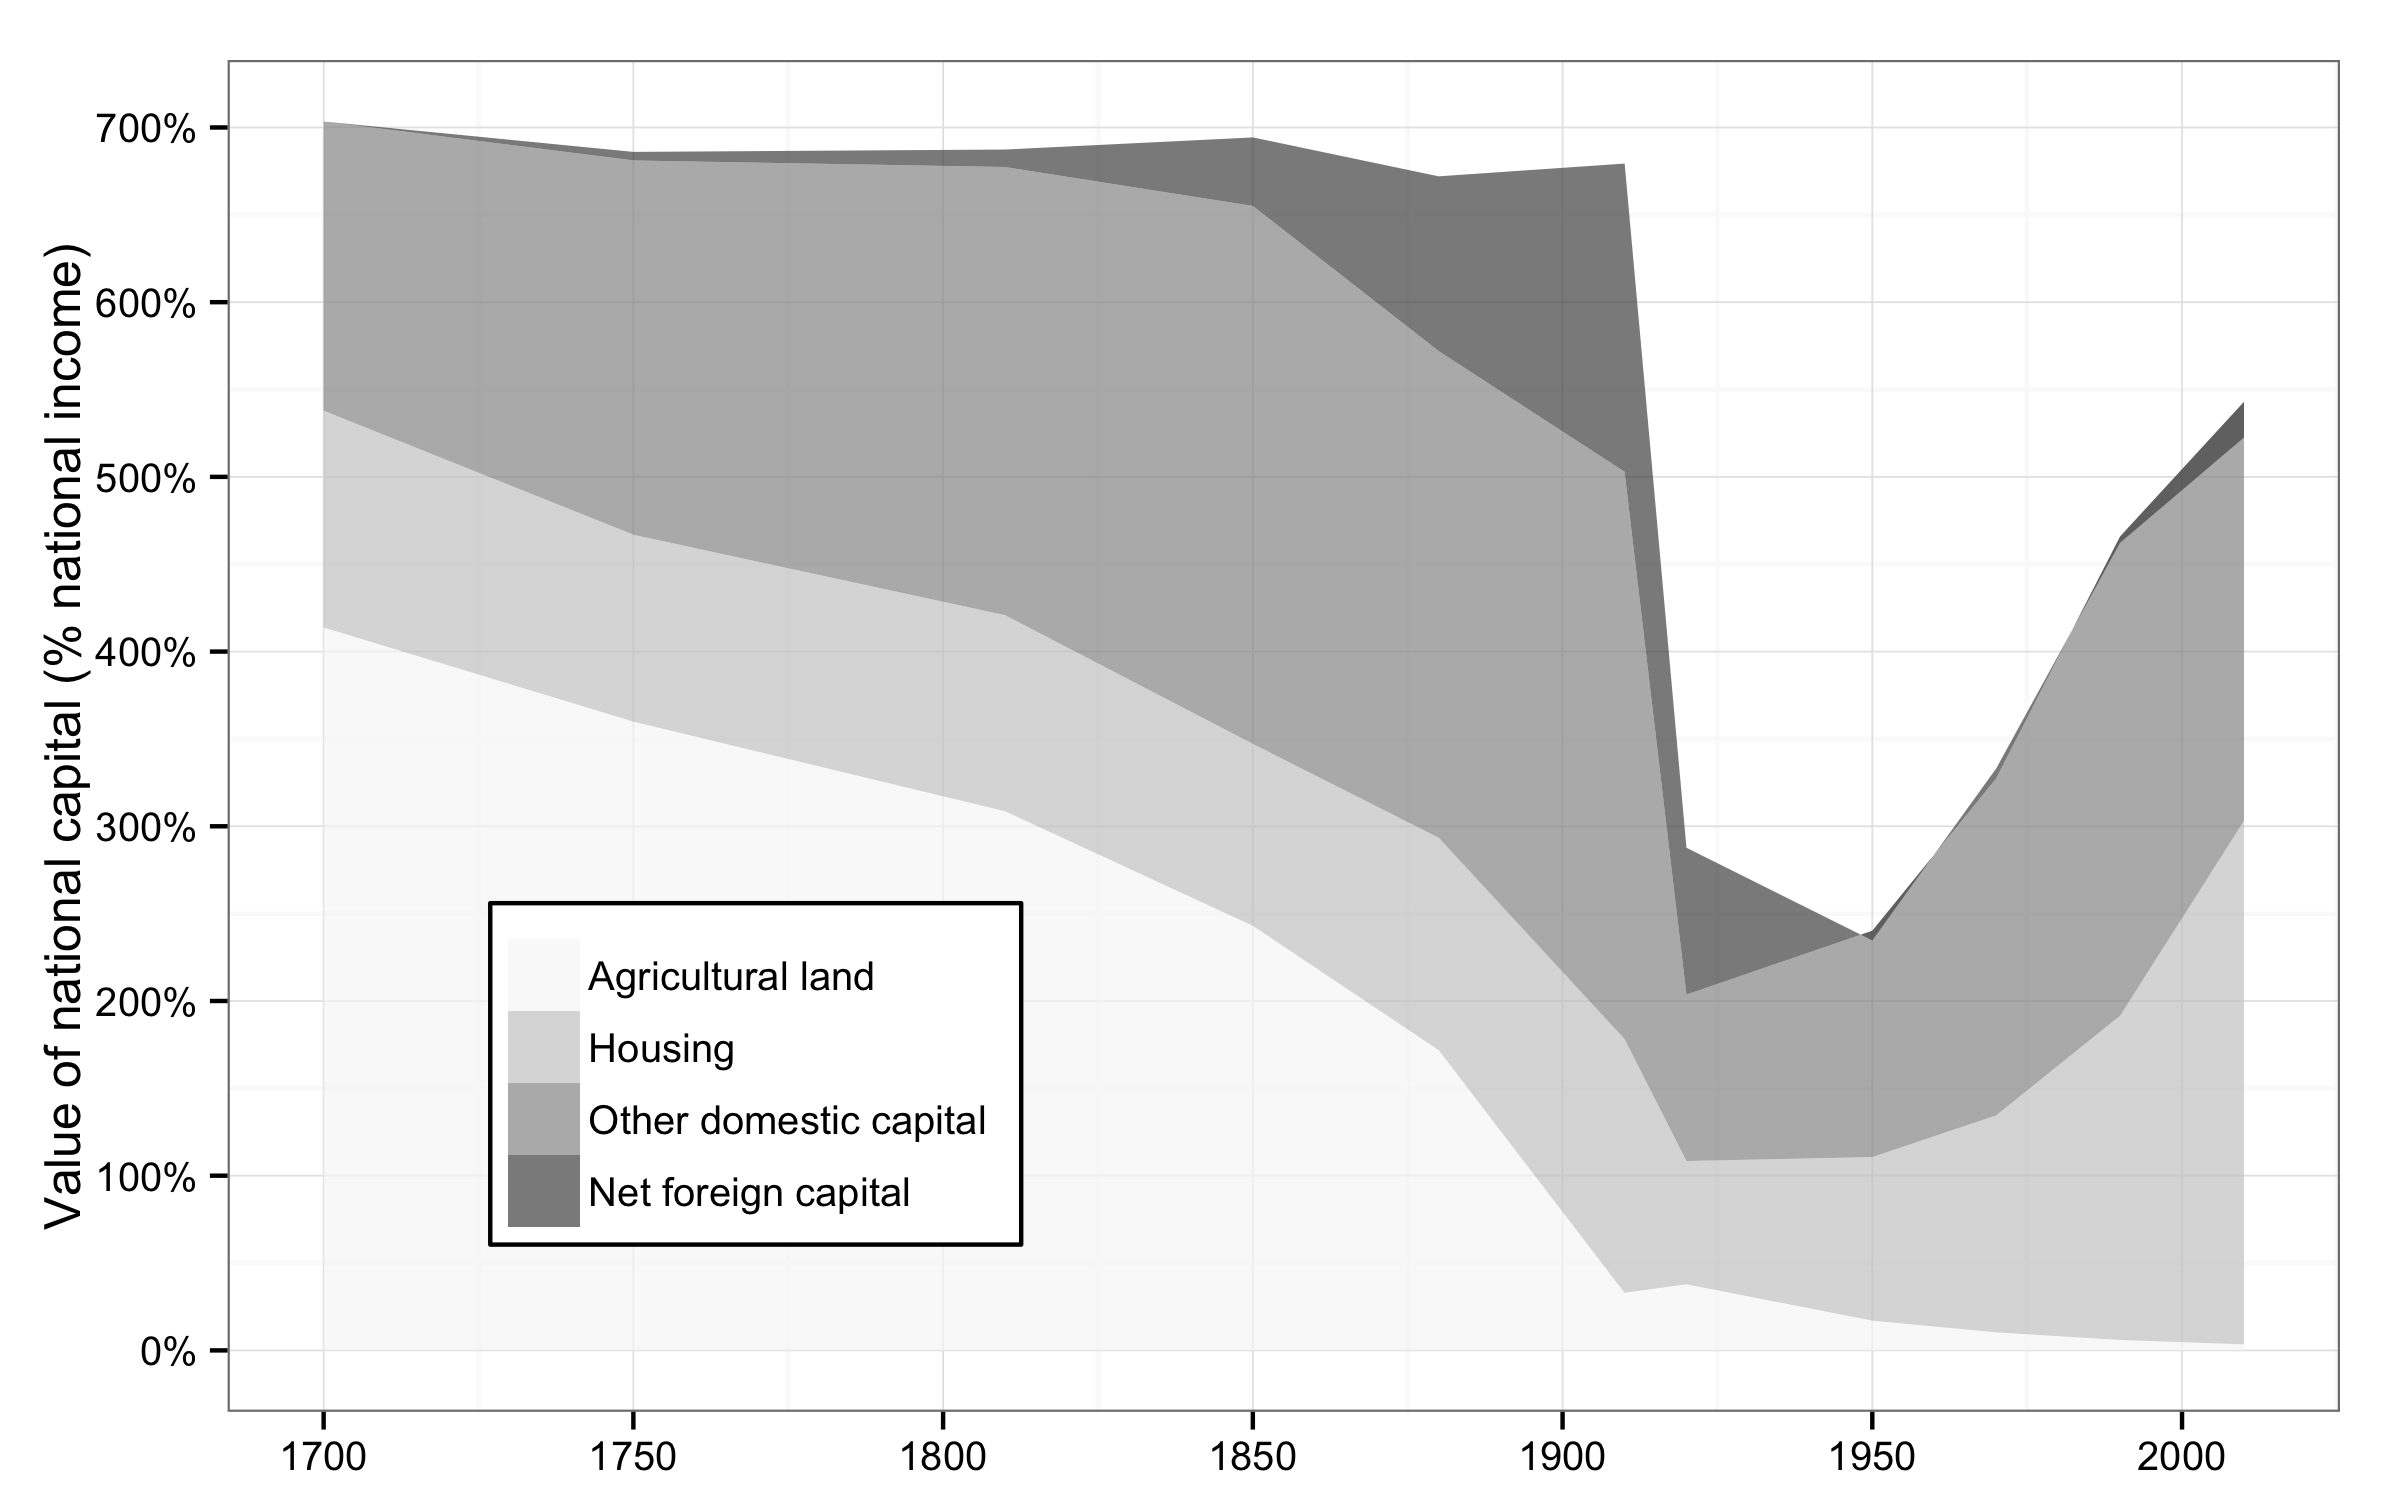
\includegraphics[width=1\linewidth]{figures/bw/Figure_3_1} 

}



\end{knitrout}
\caption{National capital is worth about seven years of national income in Britain in 1700 (including four in agricultural land).}
\end{minipage}
\end{figure}
\end{frame}
%%%%%%%%%%%%%%%%%%%% Frame Here %%%%%%%%%%%%%%%%%%%%%%%%%%%%%%%%%%%%%%%%%%%%%%%%


%%%%%%%%%%%%%%%%%%%% Frame Here %%%%%%%%%%%%%%%%%%%%%%%%%%%%%%%%%%%%%%%%%%%%%%%%
\begin{frame}[label=Figure_3_2]
\frametitle{Figure 3.2. Capital in France, 1700--2010}
\begin{figure}[t]
\begin{minipage}[b]{\textwidth}
\centering
\begin{knitrout}\footnotesize
\definecolor{shadecolor}{rgb}{0.969, 0.969, 0.969}\color{fgcolor}

{\centering 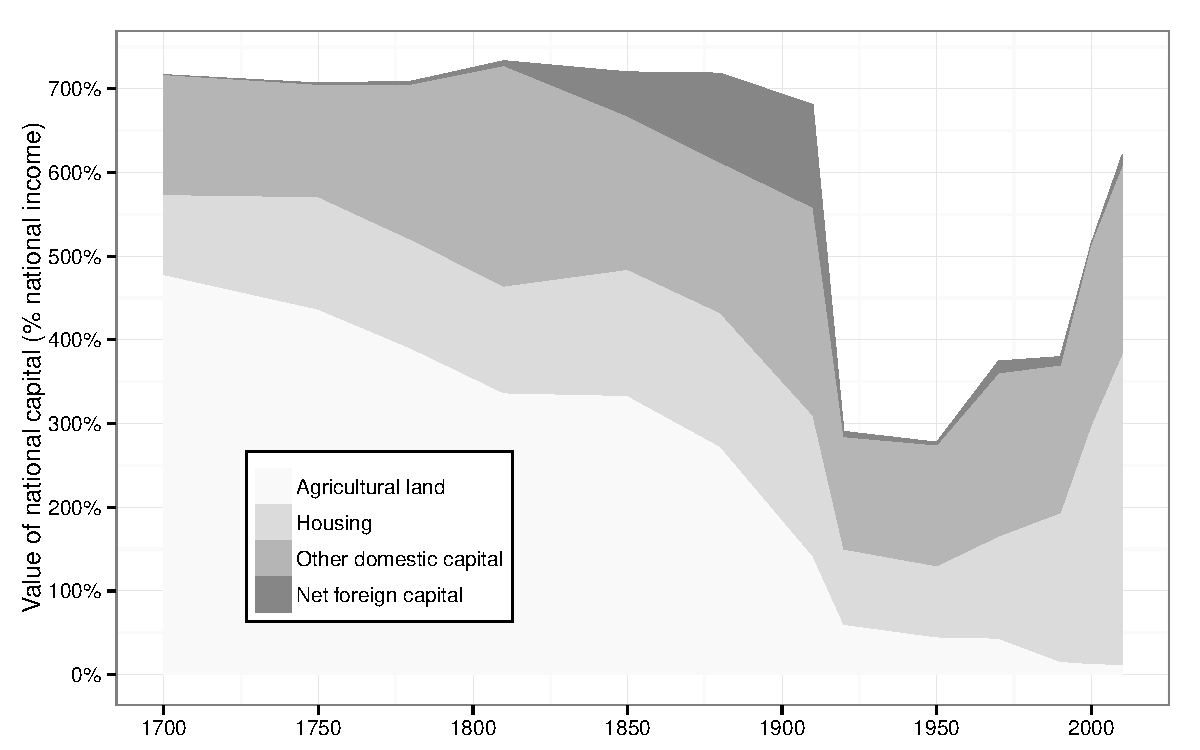
\includegraphics[width=1\linewidth]{figures/bw/Figure_3_2} 

}



\end{knitrout}
\caption{National capital is worth almost seven years of national income in France in 1910 (including one invested abroad).}
\end{minipage}
\end{figure}
\end{frame}
%%%%%%%%%%%%%%%%%%%% Frame Here %%%%%%%%%%%%%%%%%%%%%%%%%%%%%%%%%%%%%%%%%%%%%%%%


%%%%%%%%%%%%%%%%%%%% Frame Here %%%%%%%%%%%%%%%%%%%%%%%%%%%%%%%%%%%%%%%%%%%%%%%%
\begin{frame}[label=Figure_3_3]
\frametitle{Figure 3.3. Public wealth in Britain, 1700--2010}
\begin{figure}[t]
\begin{minipage}[b]{\textwidth}
\centering
\begin{knitrout}\footnotesize
\definecolor{shadecolor}{rgb}{0.969, 0.969, 0.969}\color{fgcolor}

{\centering 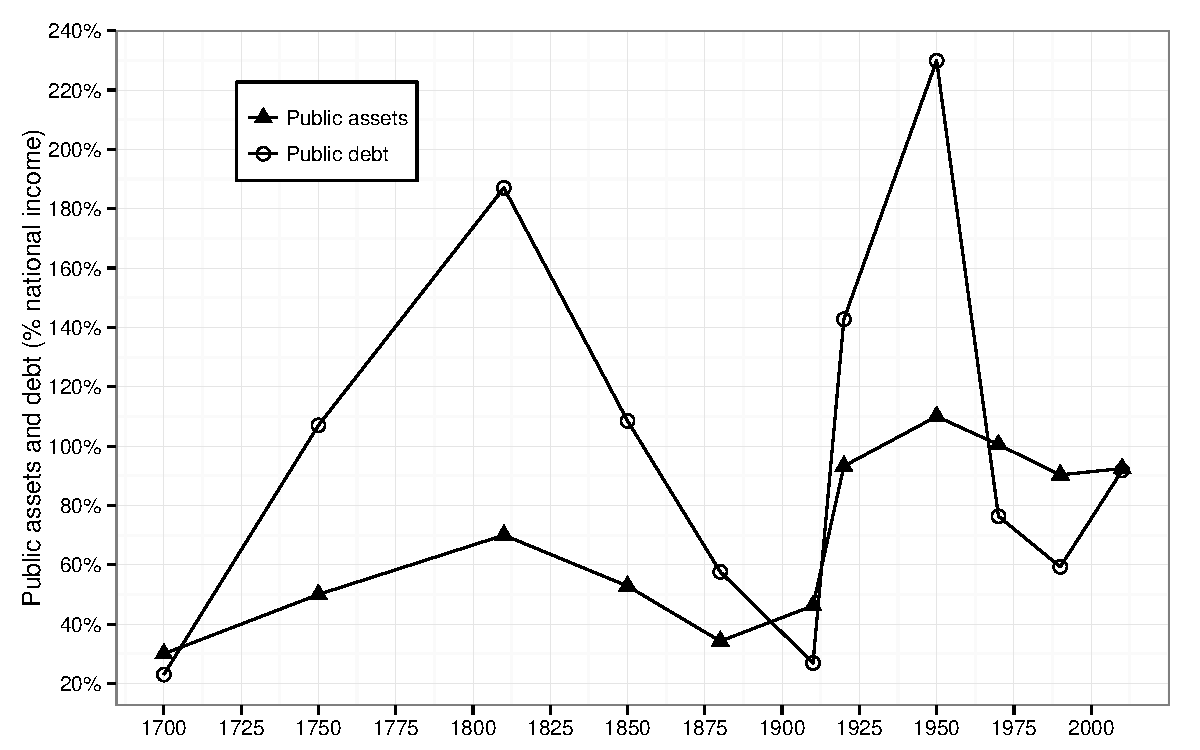
\includegraphics[width=1\linewidth]{figures/bw/Figure_3_3} 

}



\end{knitrout}
\caption{Public debt surpassed two years of national income in 1950 (versus one year for public assets).}
\end{minipage}
\end{figure}
\end{frame}
%%%%%%%%%%%%%%%%%%%% Frame Here %%%%%%%%%%%%%%%%%%%%%%%%%%%%%%%%%%%%%%%%%%%%%%%%


%%%%%%%%%%%%%%%%%%%% Frame Here %%%%%%%%%%%%%%%%%%%%%%%%%%%%%%%%%%%%%%%%%%%%%%%%
\begin{frame}[label=Figure_3_4]
\frametitle{Figure 3.4. Public wealth in France, 1700--2010}
\begin{figure}[t]
\begin{minipage}[b]{\textwidth}
\centering
\begin{knitrout}\footnotesize
\definecolor{shadecolor}{rgb}{0.969, 0.969, 0.969}\color{fgcolor}

{\centering 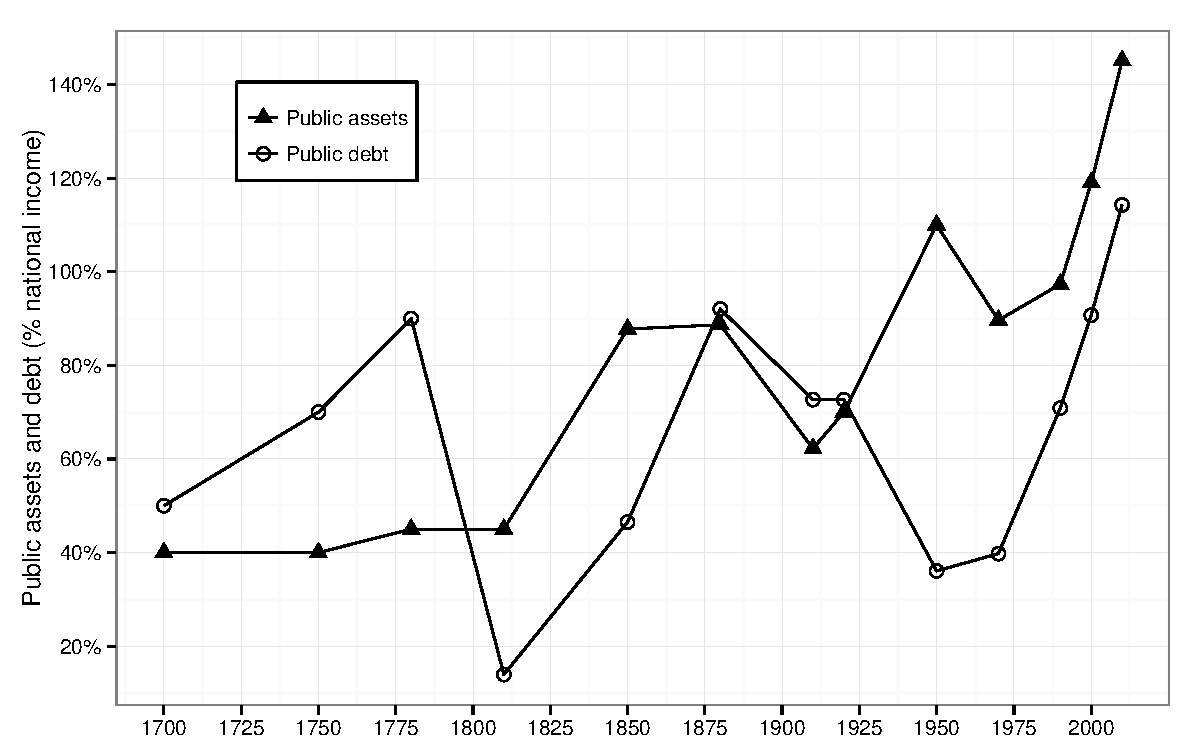
\includegraphics[width=1\linewidth]{figures/bw/Figure_3_4} 

}



\end{knitrout}
\caption{Public debt is about one year of national income in France in 1780 as well as in 1880 and in 2000--2010.}
\end{minipage}
\end{figure}
\end{frame}
%%%%%%%%%%%%%%%%%%%% Frame Here %%%%%%%%%%%%%%%%%%%%%%%%%%%%%%%%%%%%%%%%%%%%%%%%


%%%%%%%%%%%%%%%%%%%% Frame Here %%%%%%%%%%%%%%%%%%%%%%%%%%%%%%%%%%%%%%%%%%%%%%%%
\begin{frame}[label=Figure_3_5]
\frametitle{Figure 3.5. Private and public capital in Britain, 1700--2010}
\begin{figure}[t]
\begin{minipage}[b]{\textwidth}
\centering
\begin{knitrout}\footnotesize
\definecolor{shadecolor}{rgb}{0.969, 0.969, 0.969}\color{fgcolor}

{\centering 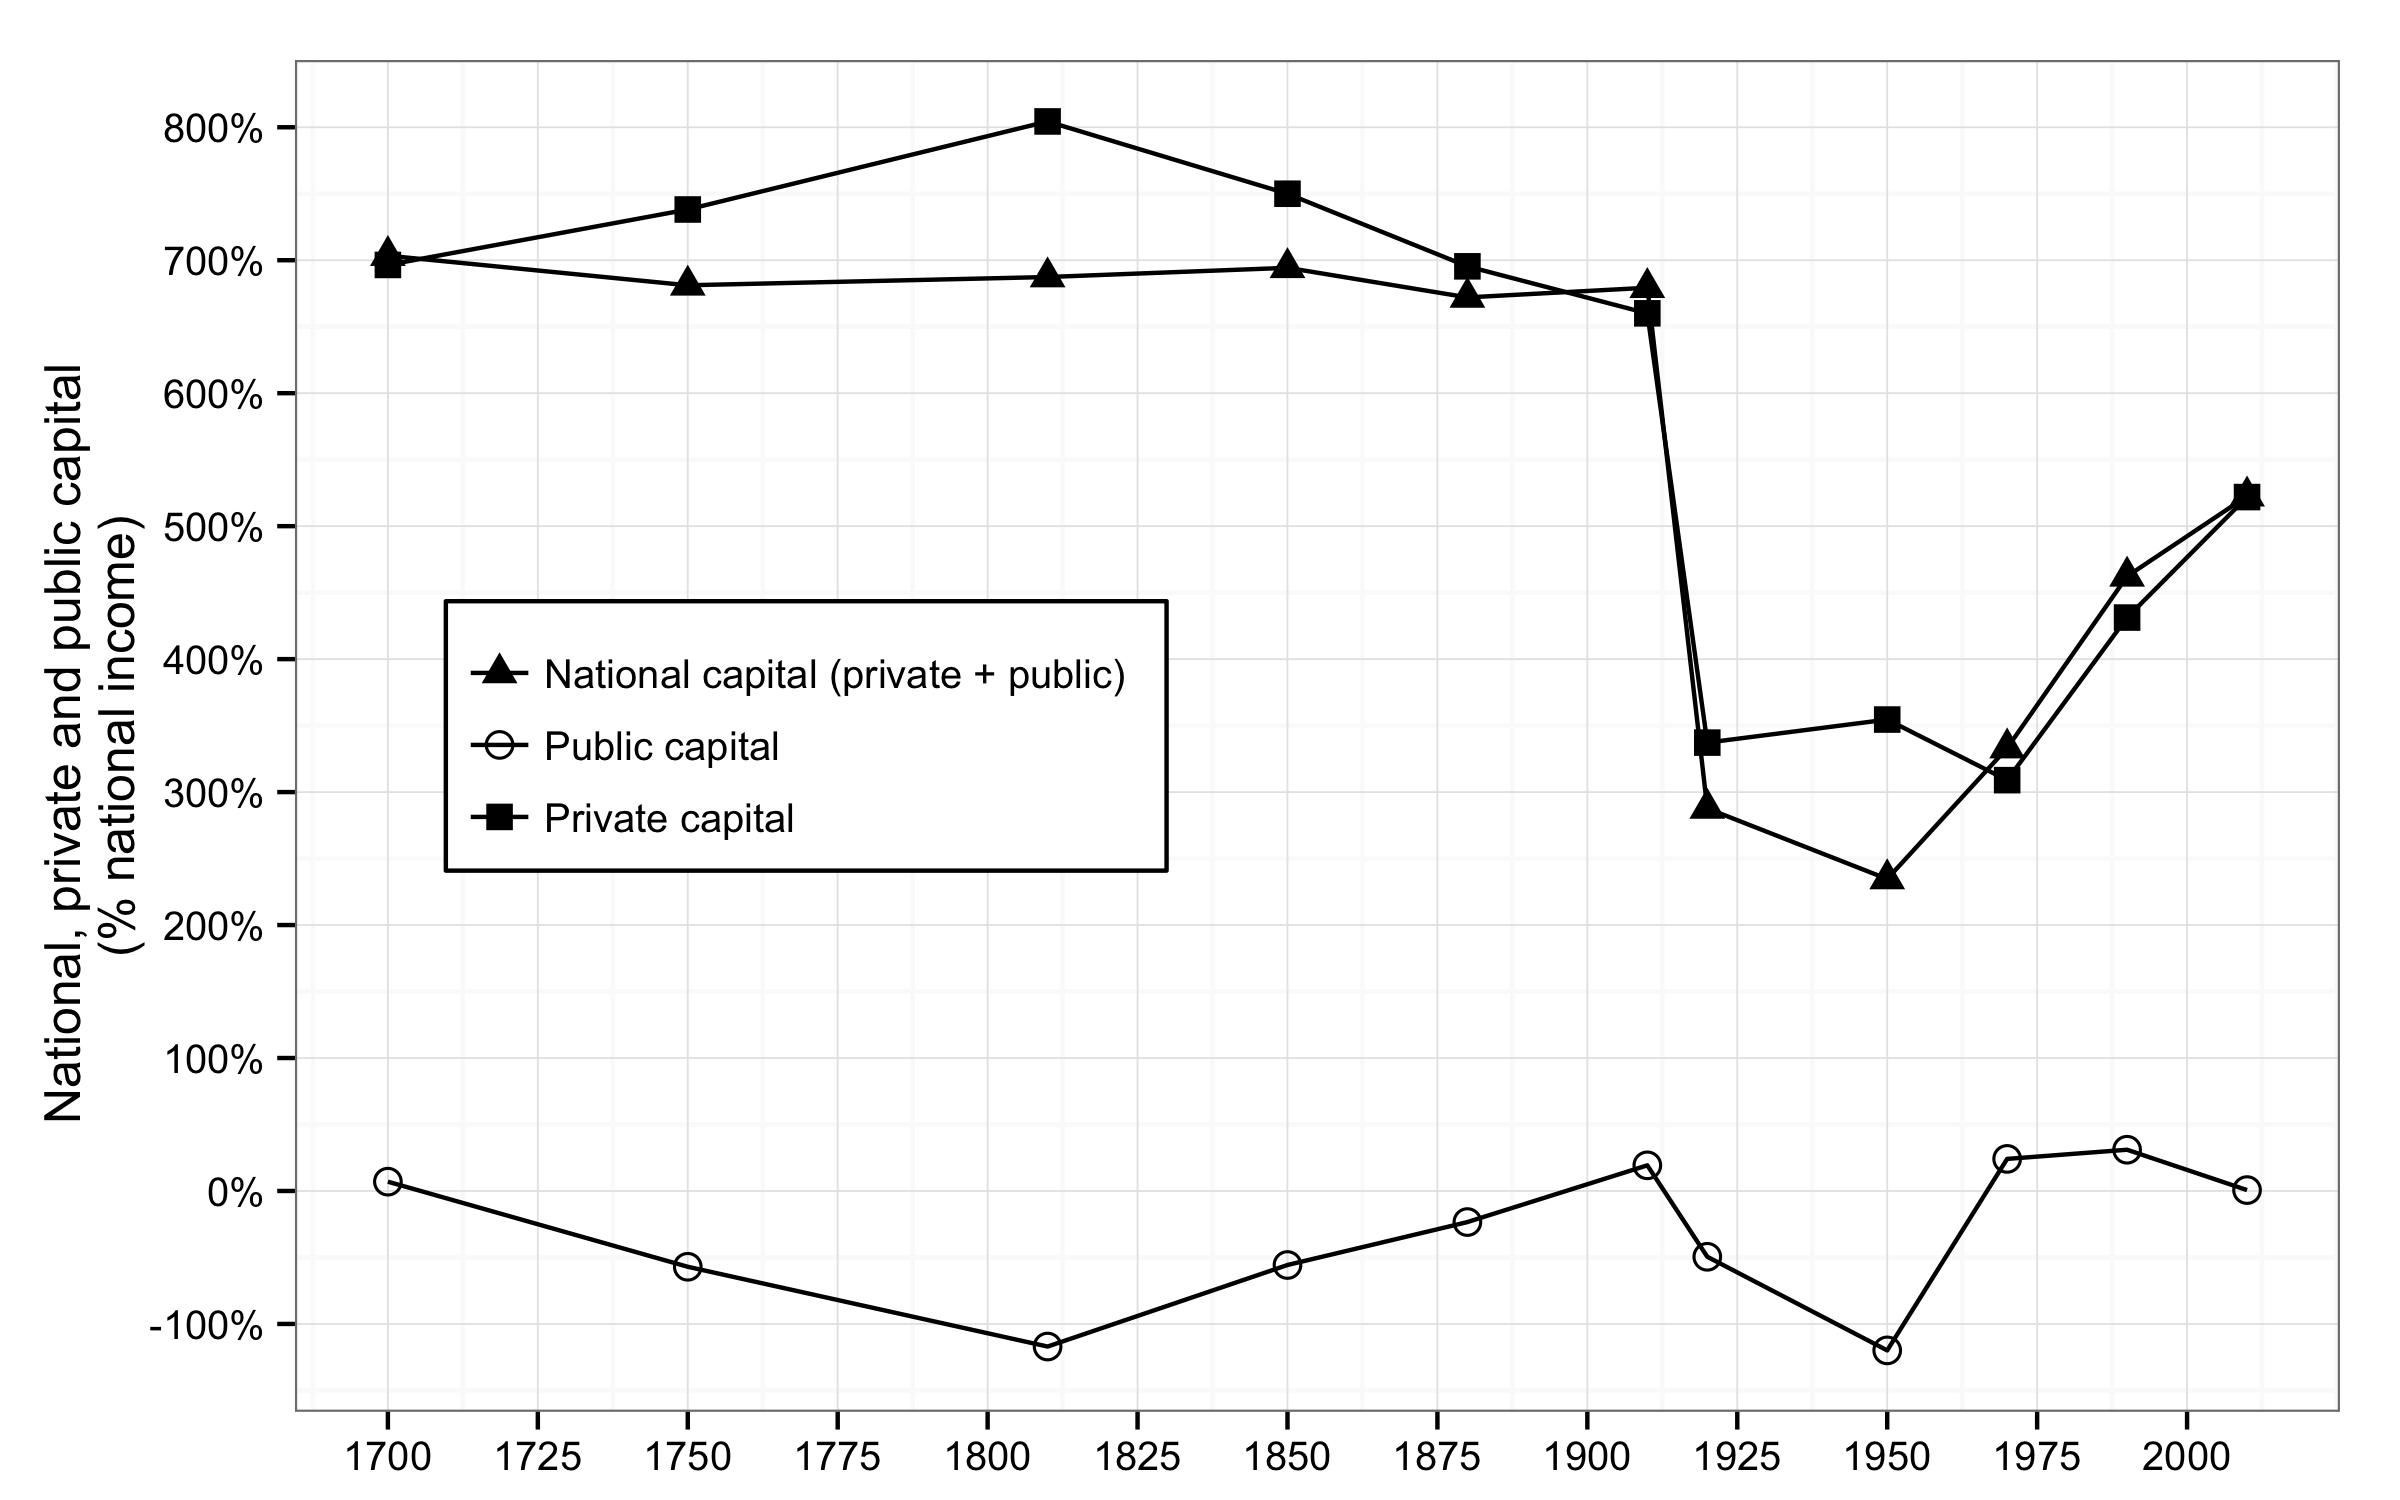
\includegraphics[width=1\linewidth]{figures/bw/Figure_3_5} 

}



\end{knitrout}
\caption{In 1810, private capital is worth eight years of national income in Britain (versus seven years for national capital).}
\end{minipage}
\end{figure}
\end{frame}
%%%%%%%%%%%%%%%%%%%% Frame Here %%%%%%%%%%%%%%%%%%%%%%%%%%%%%%%%%%%%%%%%%%%%%%%%


%%%%%%%%%%%%%%%%%%%% Frame Here %%%%%%%%%%%%%%%%%%%%%%%%%%%%%%%%%%%%%%%%%%%%%%%%
\begin{frame}[label=Figure_3_6]
\frametitle{Figure 3.6. Private and public capital in France, 1700--2010}
\begin{figure}[t]
\begin{minipage}[b]{\textwidth}
\centering
\begin{knitrout}\footnotesize
\definecolor{shadecolor}{rgb}{0.969, 0.969, 0.969}\color{fgcolor}

{\centering 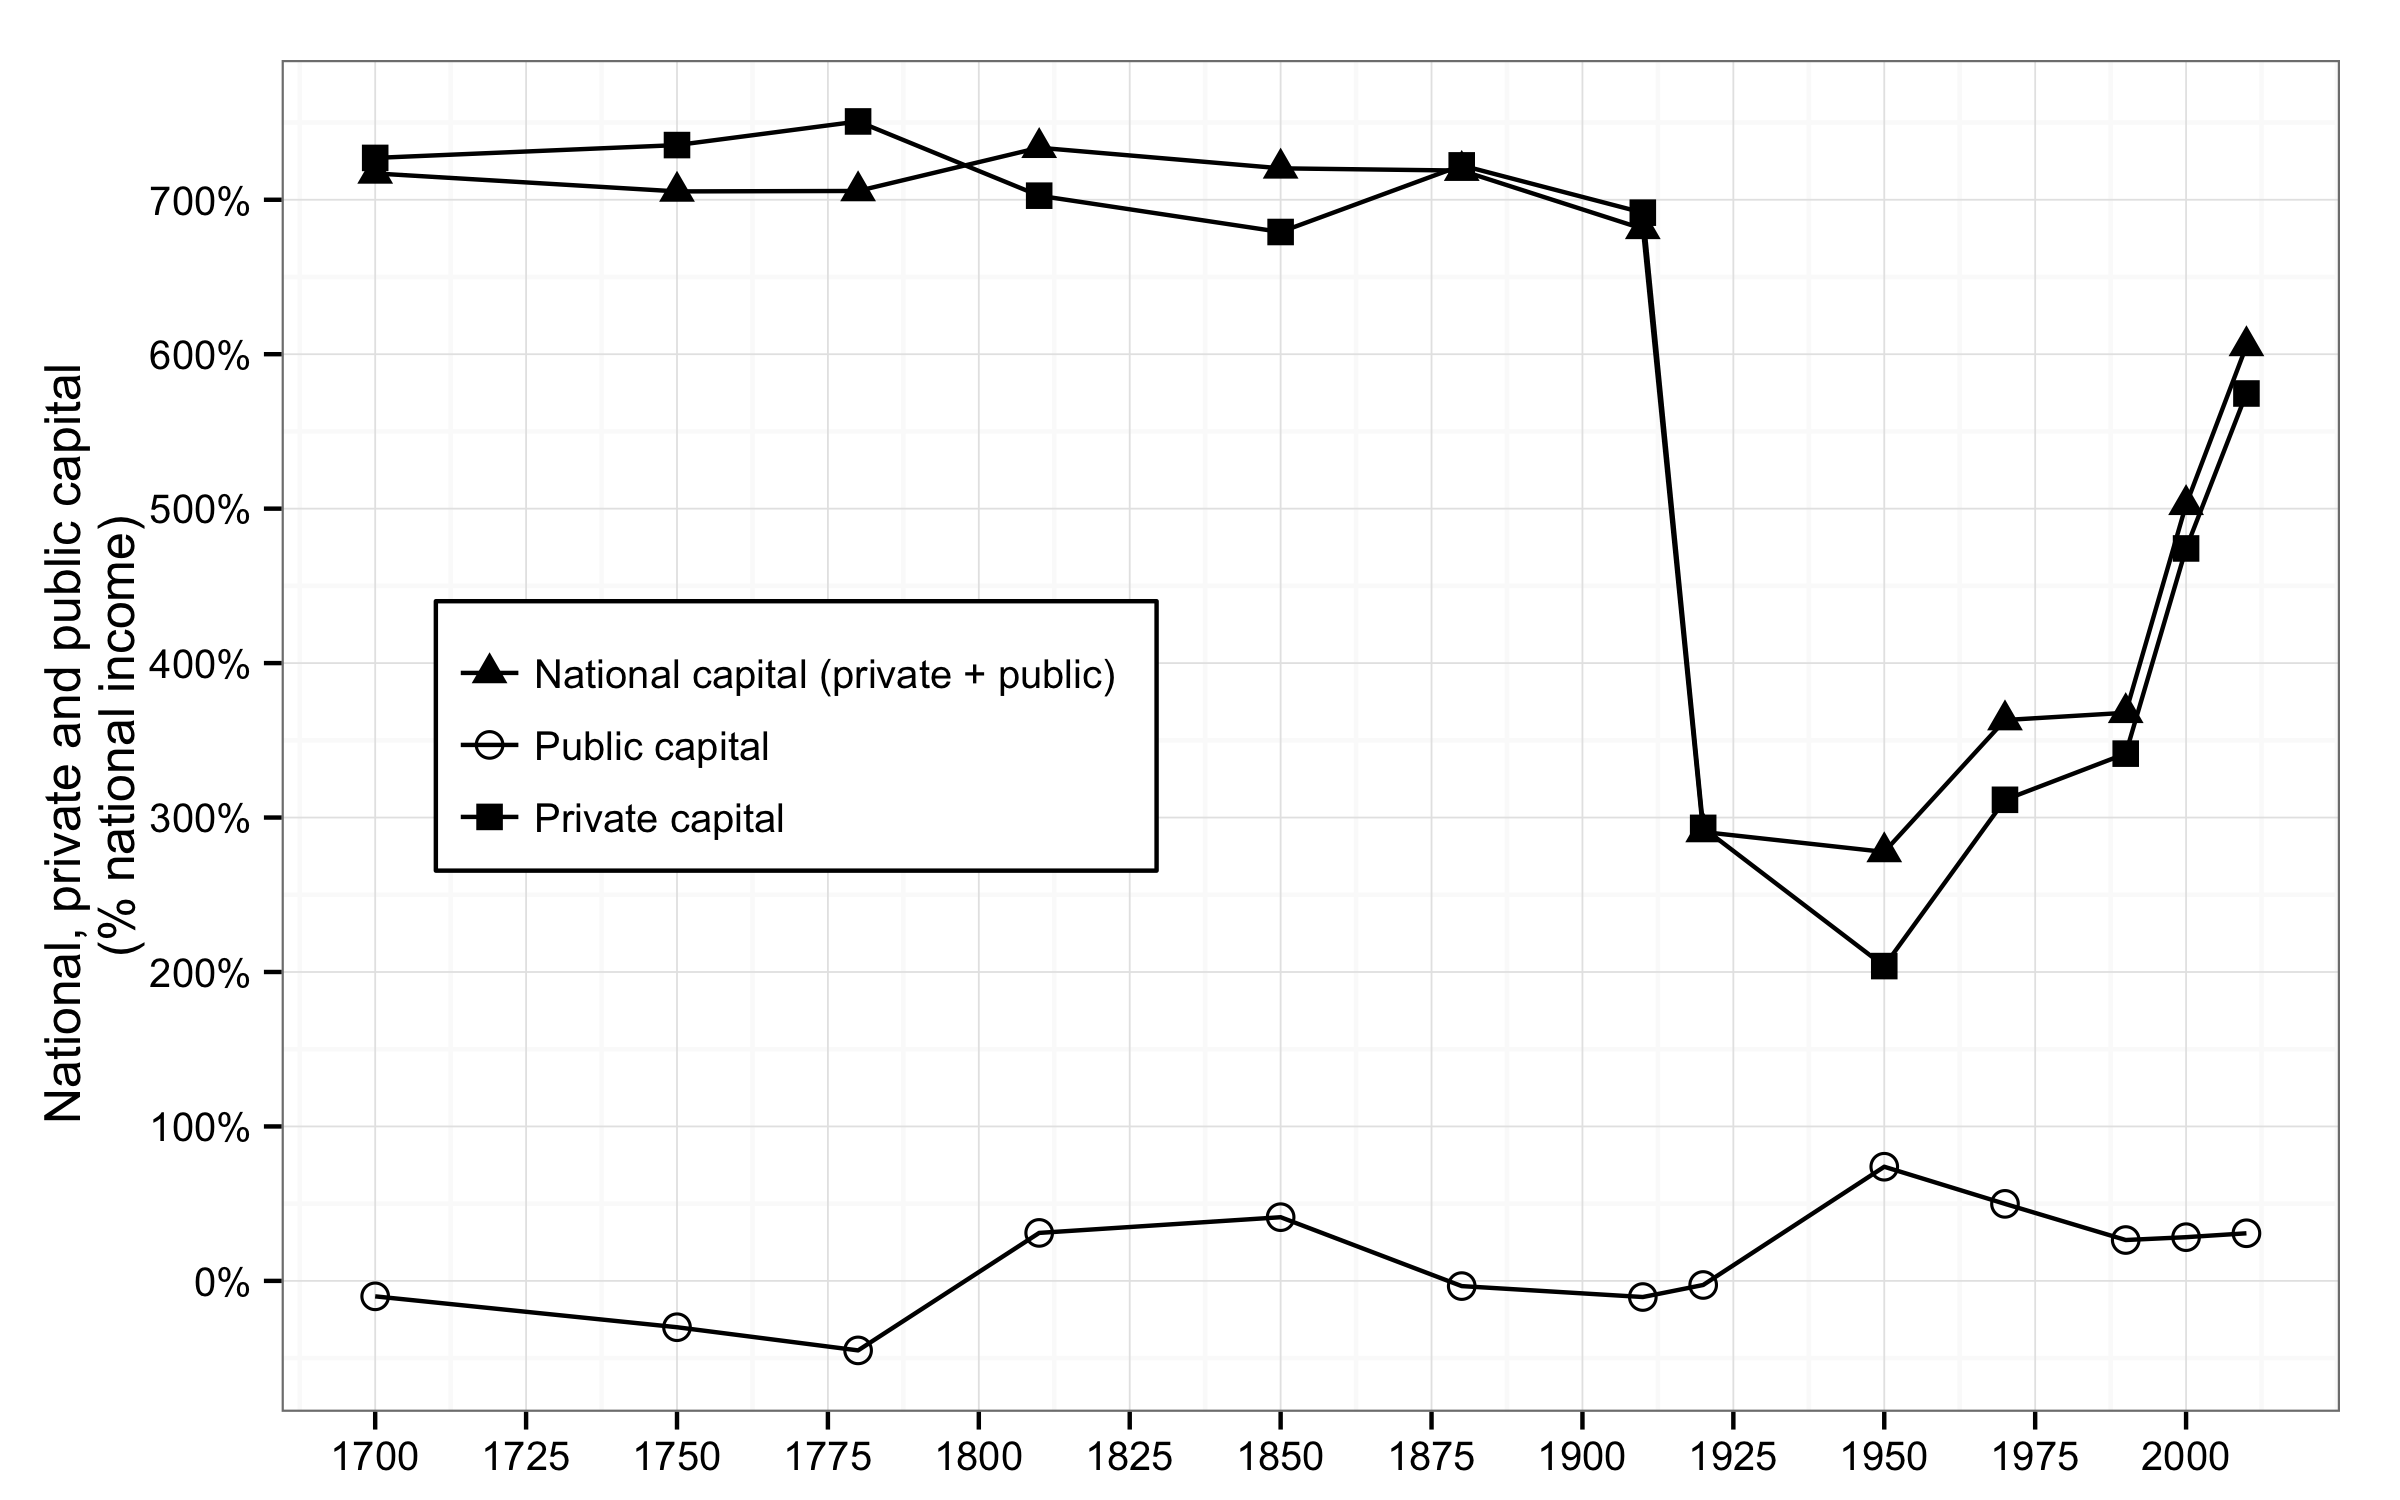
\includegraphics[width=1\linewidth]{figures/bw/Figure_3_6} 

}



\end{knitrout}
\caption{In 1950, public capital is worth almost one year of national income versus two years for private capital.}
\end{minipage}
\end{figure}
\end{frame}
%%%%%%%%%%%%%%%%%%%% Frame Here %%%%%%%%%%%%%%%%%%%%%%%%%%%%%%%%%%%%%%%%%%%%%%%%


%%%%%%%%%%%%%%%%%%%% Frame Here %%%%%%%%%%%%%%%%%%%%%%%%%%%%%%%%%%%%%%%%%%%%%%%%
\begin{frame}[label=Figure_4_1]
\frametitle{Figure 4.1. Capital in Germany, 1870--2010}
\begin{figure}[t]
\begin{minipage}[b]{\textwidth}
\centering
\begin{knitrout}\footnotesize
\definecolor{shadecolor}{rgb}{0.969, 0.969, 0.969}\color{fgcolor}

{\centering 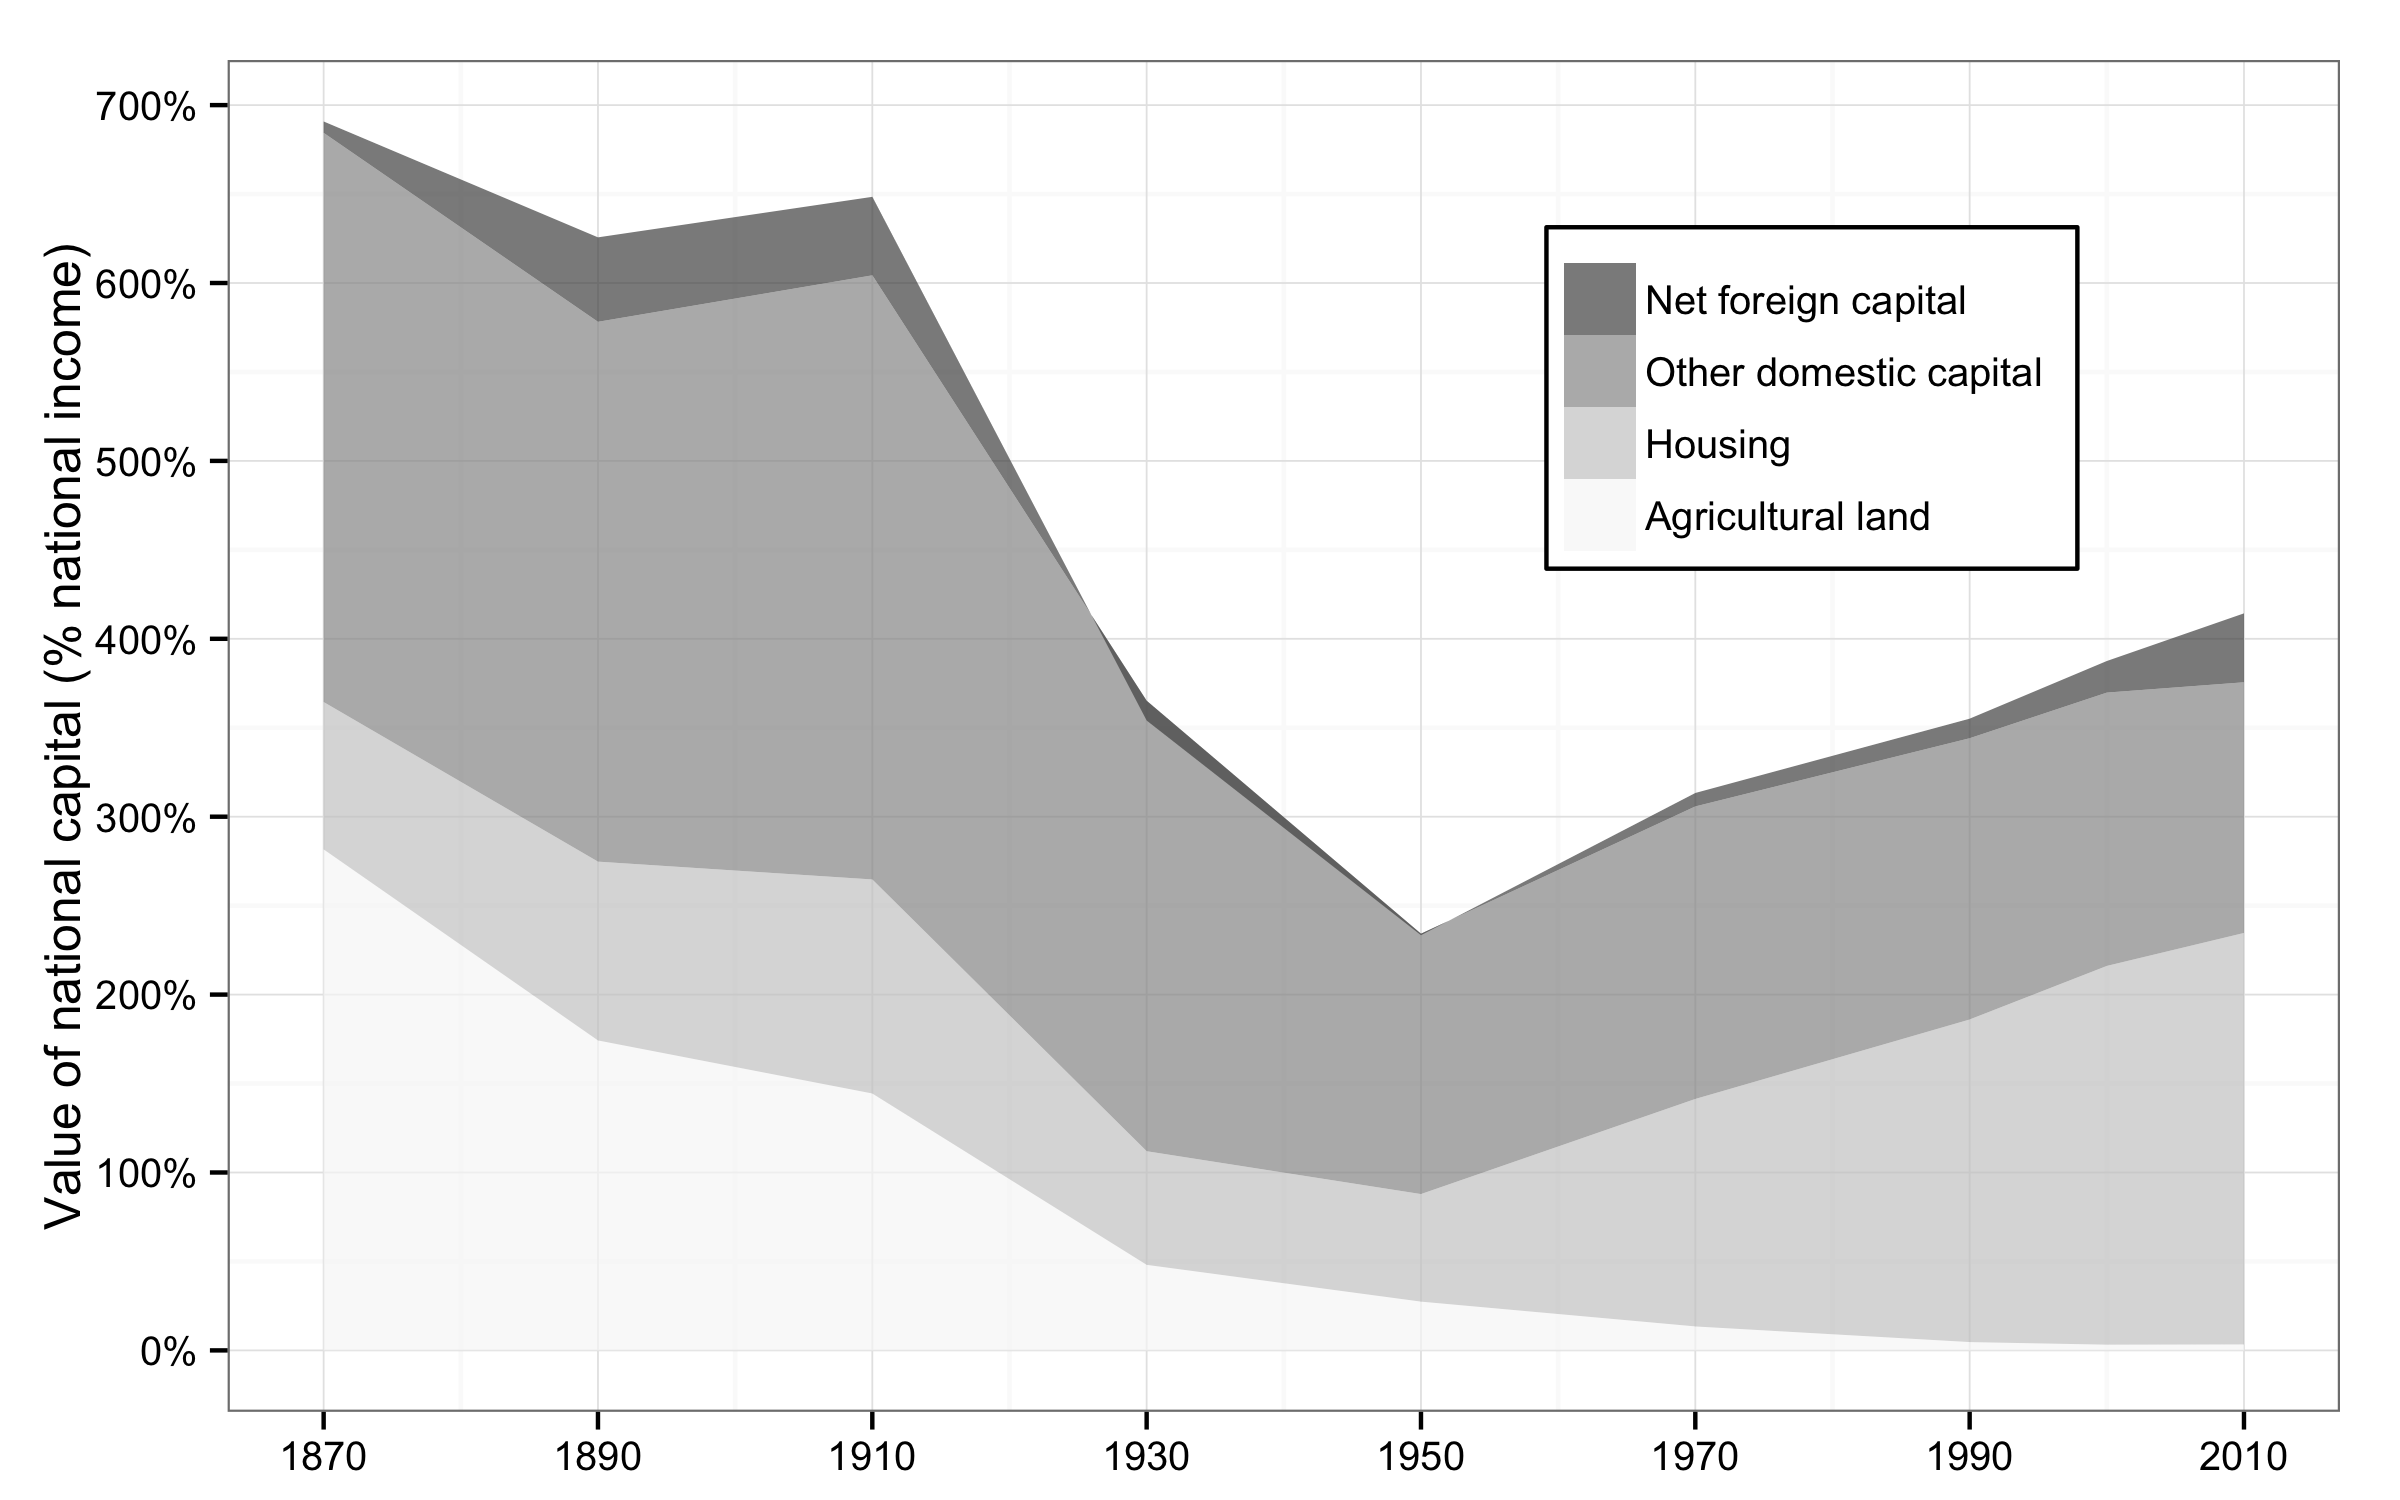
\includegraphics[width=1\linewidth]{figures/bw/Figure_4_1} 

}



\end{knitrout}
\caption{National capital is worth 6.5 years of national income in Germany in 1910 (including about 0.5 year invested abroad).}
\end{minipage}
\end{figure}
\end{frame}
%%%%%%%%%%%%%%%%%%%% Frame Here %%%%%%%%%%%%%%%%%%%%%%%%%%%%%%%%%%%%%%%%%%%%%%%%


%%%%%%%%%%%%%%%%%%%% Frame Here %%%%%%%%%%%%%%%%%%%%%%%%%%%%%%%%%%%%%%%%%%%%%%%%
\begin{frame}[label=Figure_4_2]
\frametitle{Figure 4.2. Public wealth in Germany, 1870--2010}
\begin{figure}[t]
\begin{minipage}[b]{\textwidth}
\centering
\begin{knitrout}\footnotesize
\definecolor{shadecolor}{rgb}{0.969, 0.969, 0.969}\color{fgcolor}

{\centering 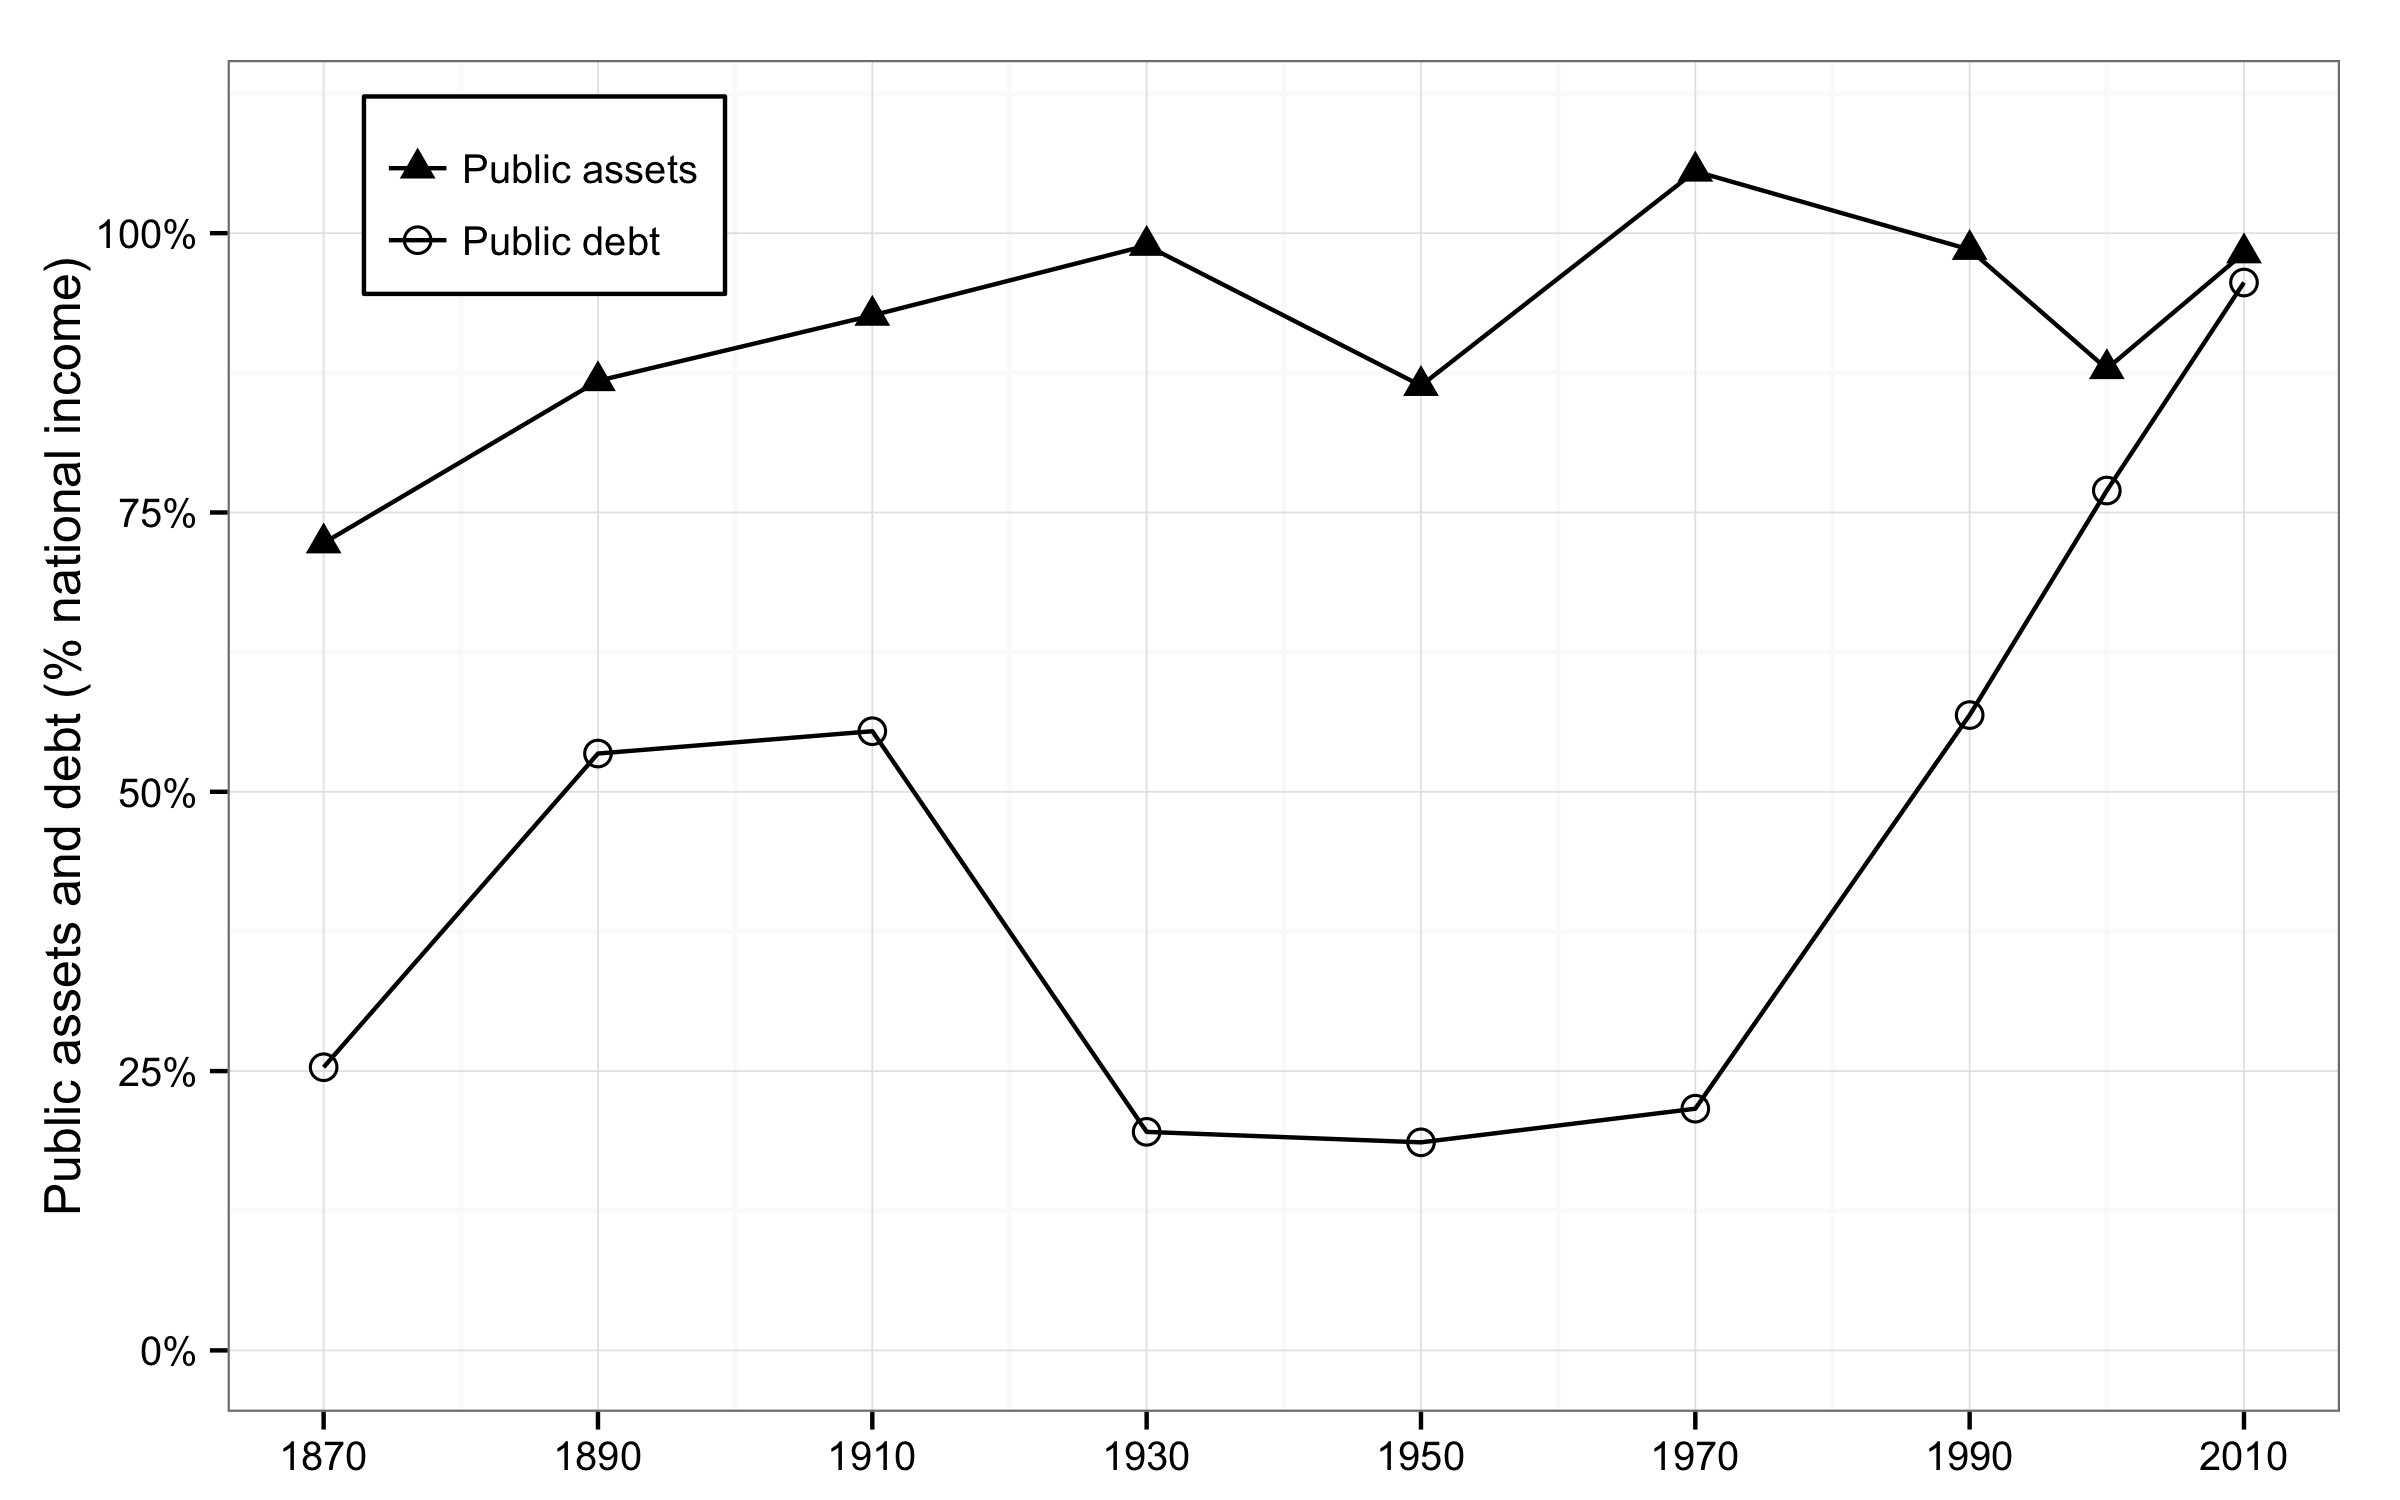
\includegraphics[width=1\linewidth]{figures/bw/Figure_4_2} 

}



\end{knitrout}
\caption{Public debt is worth almost one year of national income in Germany in 2010 (as much as assets).}
\end{minipage}
\end{figure}
\end{frame}
%%%%%%%%%%%%%%%%%%%% Frame Here %%%%%%%%%%%%%%%%%%%%%%%%%%%%%%%%%%%%%%%%%%%%%%%%


%%%%%%%%%%%%%%%%%%%% Frame Here %%%%%%%%%%%%%%%%%%%%%%%%%%%%%%%%%%%%%%%%%%%%%%%%
\begin{frame}[label=Figure_4_3]
\frametitle{Figure 4.3. Private and public capital in Germany, 1870--2010}
\begin{figure}[t]
\begin{minipage}[b]{\textwidth}
\centering
\begin{knitrout}\footnotesize
\definecolor{shadecolor}{rgb}{0.969, 0.969, 0.969}\color{fgcolor}

{\centering 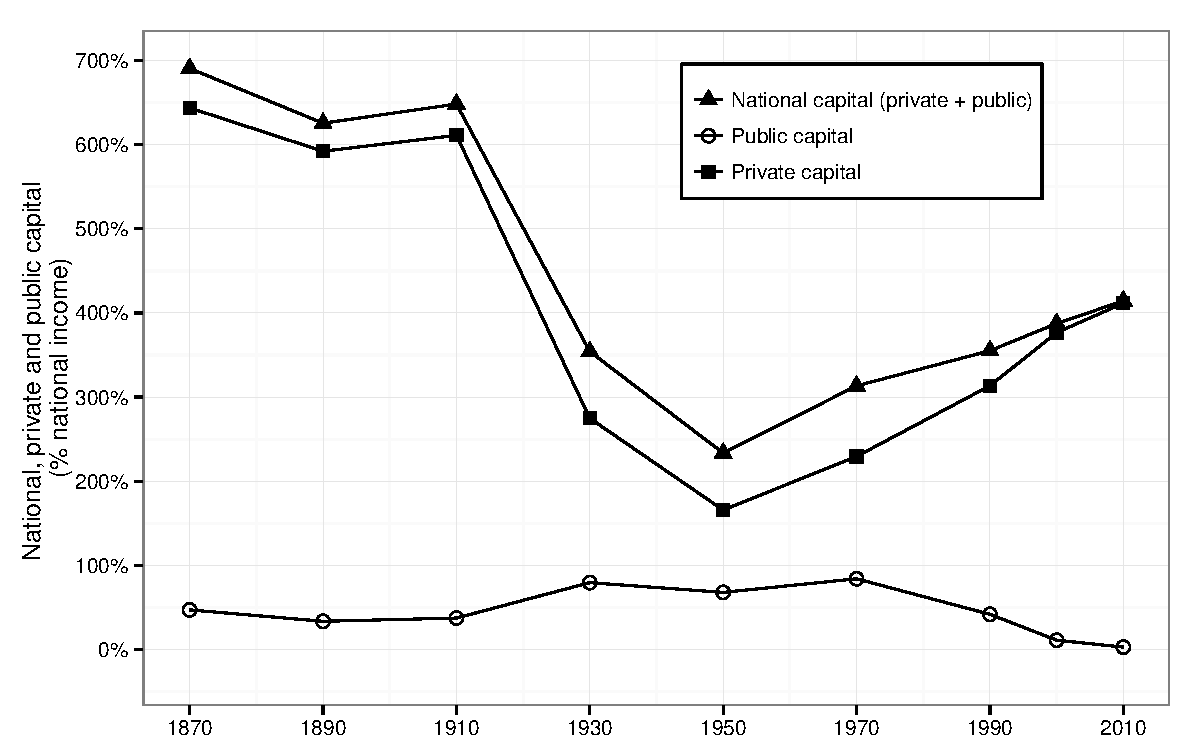
\includegraphics[width=1\linewidth]{figures/bw/Figure_4_3} 

}



\end{knitrout}
\caption{In 1970, public capital is worth almost one year of national income, versus slightly more than two for private capital.}
\end{minipage}
\end{figure}
\end{frame}
%%%%%%%%%%%%%%%%%%%% Frame Here %%%%%%%%%%%%%%%%%%%%%%%%%%%%%%%%%%%%%%%%%%%%%%%%


%%%%%%%%%%%%%%%%%%%% Frame Here %%%%%%%%%%%%%%%%%%%%%%%%%%%%%%%%%%%%%%%%%%%%%%%%
\begin{frame}[label=Figure_4_4]
\frametitle{Figure 4.4. Private and public capital in Europe, 1870--2010}
\begin{figure}[t]
\begin{minipage}[b]{\textwidth}
\centering
\begin{knitrout}\footnotesize
\definecolor{shadecolor}{rgb}{0.969, 0.969, 0.969}\color{fgcolor}

{\centering 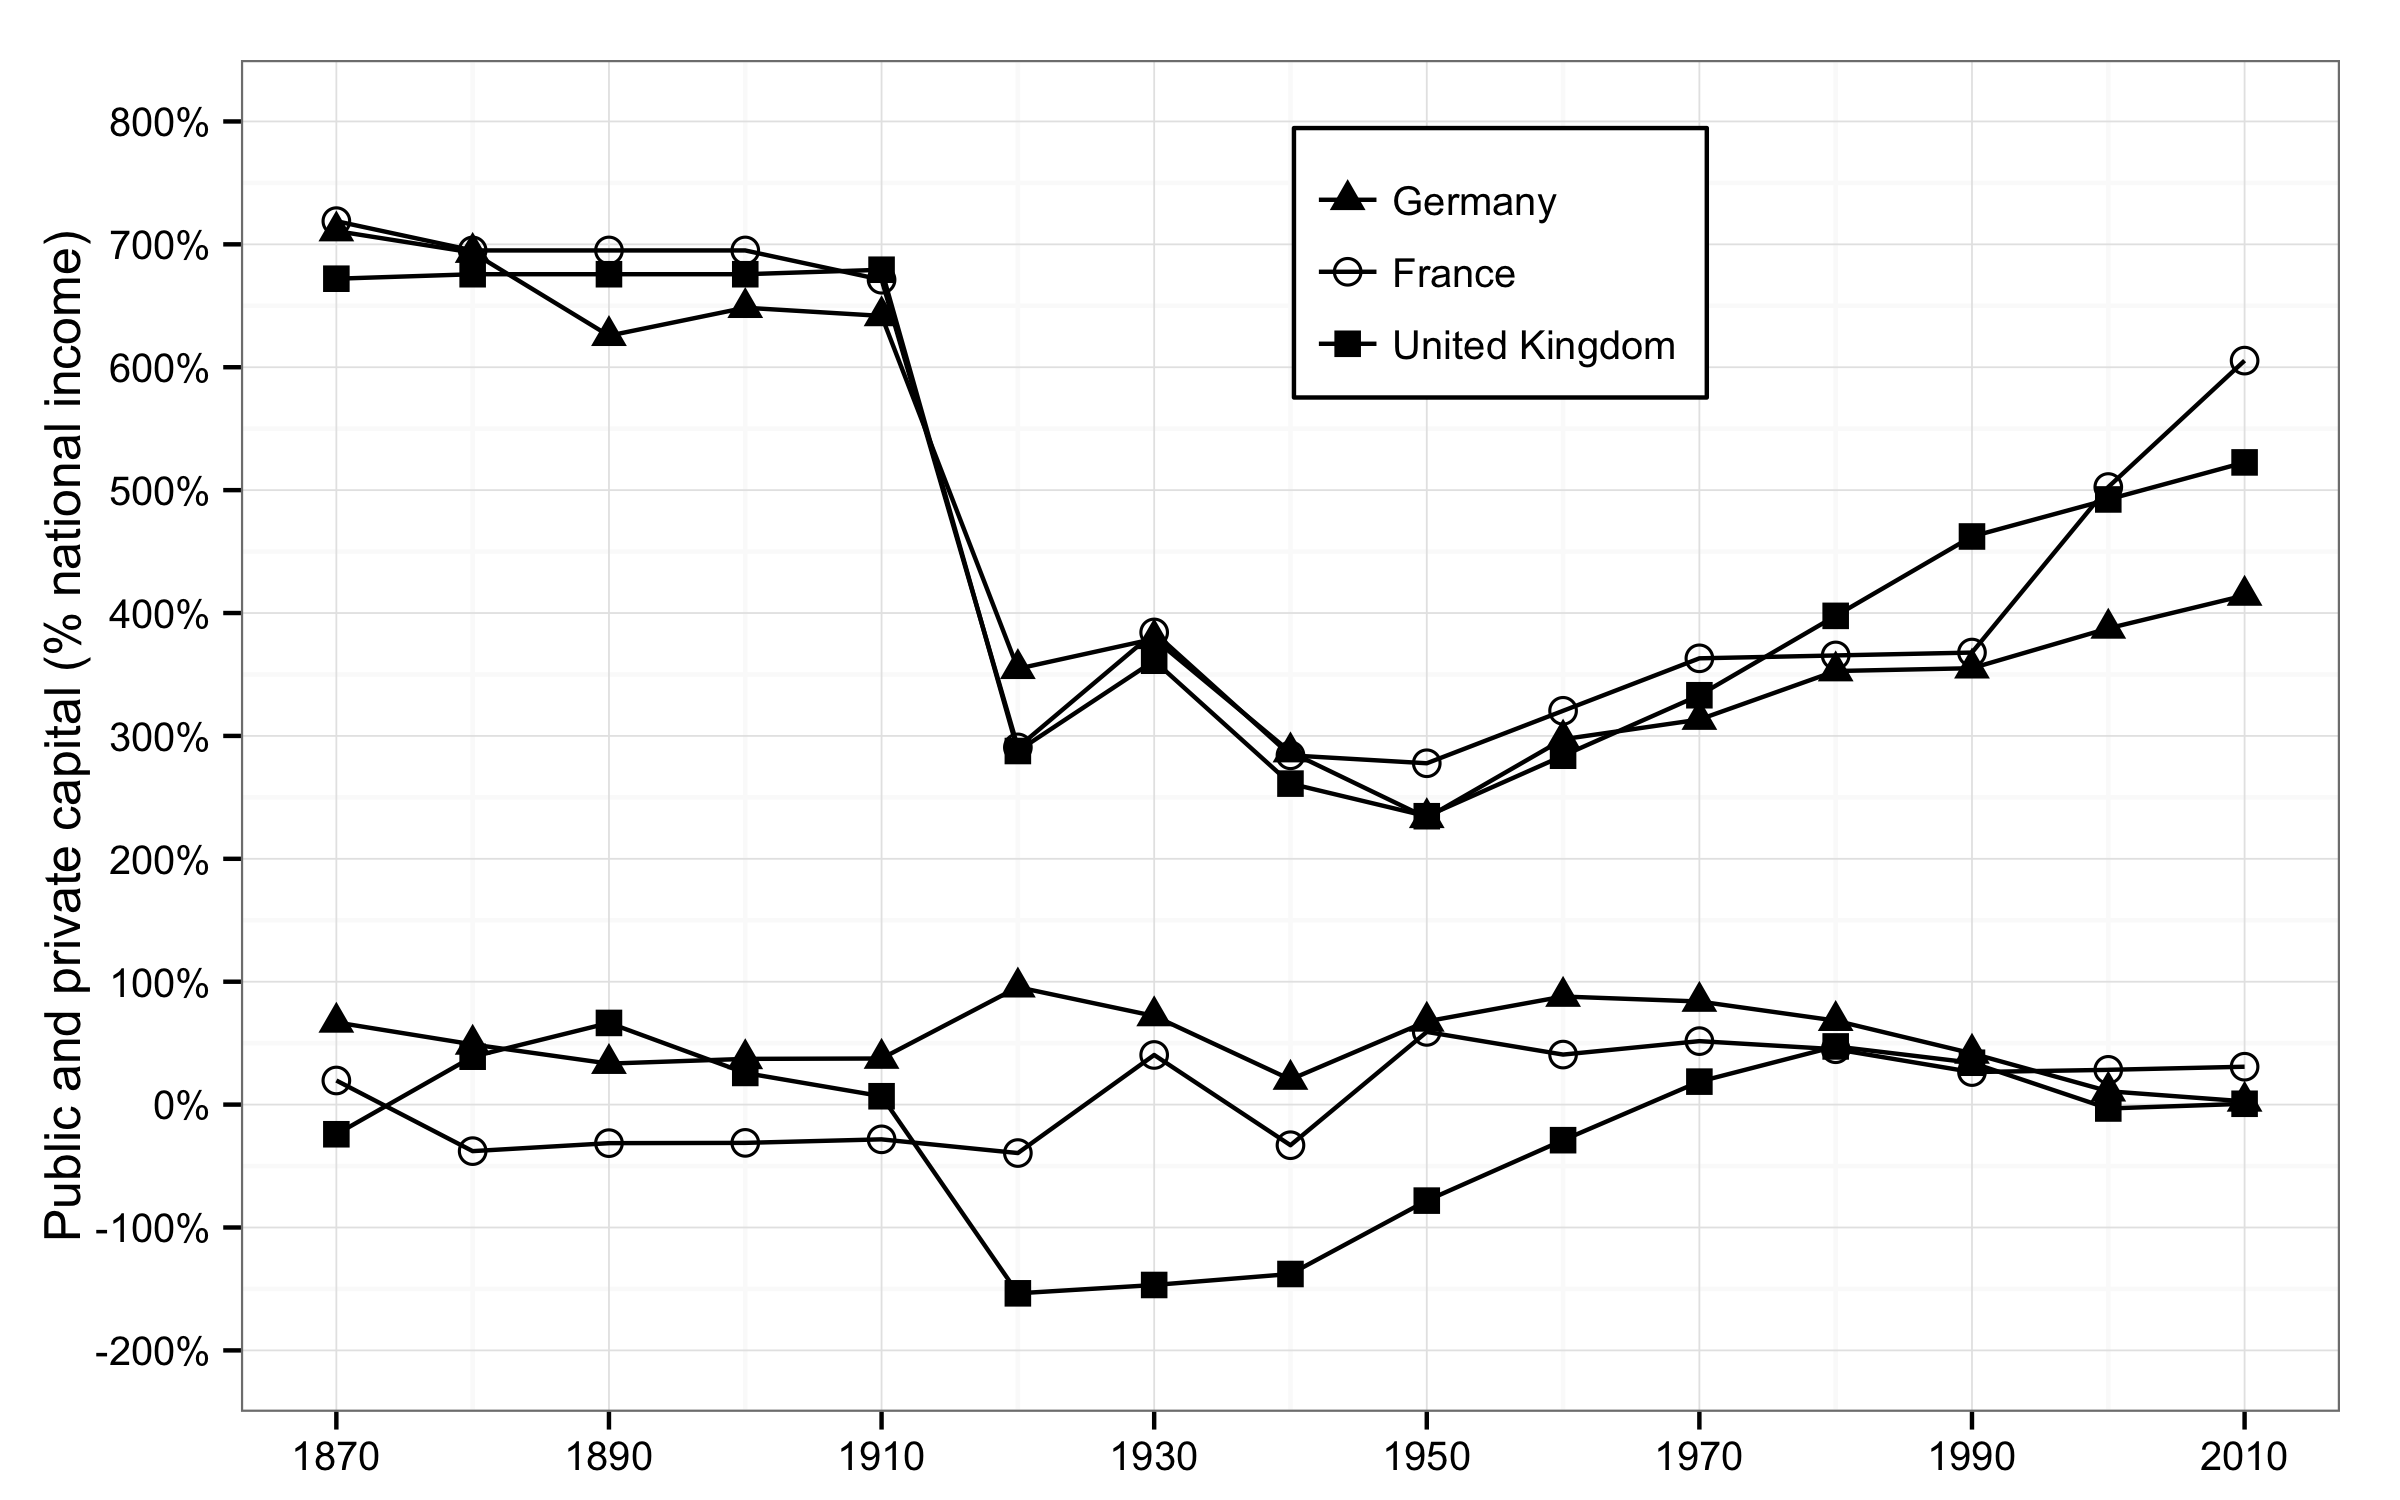
\includegraphics[width=1\linewidth]{figures/bw/Figure_4_4} 

}



\end{knitrout}
\caption{The fluctuations of national capital in Europe in the long run are mostly due to the fluctuations of private capital.}
\end{minipage}
\end{figure}
\end{frame}
%%%%%%%%%%%%%%%%%%%% Frame Here %%%%%%%%%%%%%%%%%%%%%%%%%%%%%%%%%%%%%%%%%%%%%%%%


%%%%%%%%%%%%%%%%%%%% Frame Here %%%%%%%%%%%%%%%%%%%%%%%%%%%%%%%%%%%%%%%%%%%%%%%%
\begin{frame}[label=Figure_4_5]
\frametitle{Figure 4.5. National capital in Europe, 1870--2010}
\begin{figure}[t]
\begin{minipage}[b]{\textwidth}
\centering
\begin{knitrout}\footnotesize
\definecolor{shadecolor}{rgb}{0.969, 0.969, 0.969}\color{fgcolor}

{\centering 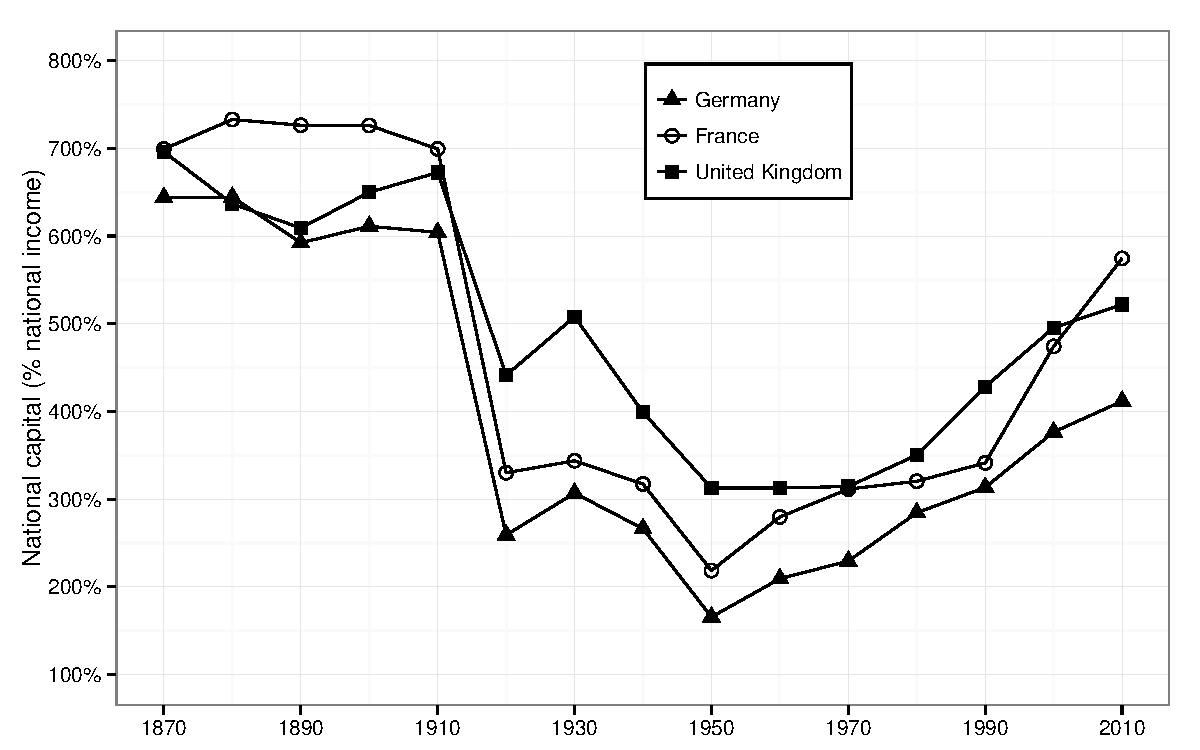
\includegraphics[width=1\linewidth]{figures/bw/Figure_4_5} 

}



\end{knitrout}
\caption{National capital (sum of public and private capital) is worth between two and three years of national income in Europe in 1950.}
\end{minipage}
\end{figure}
\end{frame}
%%%%%%%%%%%%%%%%%%%% Frame Here %%%%%%%%%%%%%%%%%%%%%%%%%%%%%%%%%%%%%%%%%%%%%%%%


%%%%%%%%%%%%%%%%%%%% Frame Here %%%%%%%%%%%%%%%%%%%%%%%%%%%%%%%%%%%%%%%%%%%%%%%%
\begin{frame}[label=Figure_4_6]
\frametitle{Figure 4.6. Capital in the United States, 1770--2010}
\begin{figure}[t]
\begin{minipage}[b]{\textwidth}
\centering
\begin{knitrout}\footnotesize
\definecolor{shadecolor}{rgb}{0.969, 0.969, 0.969}\color{fgcolor}

{\centering 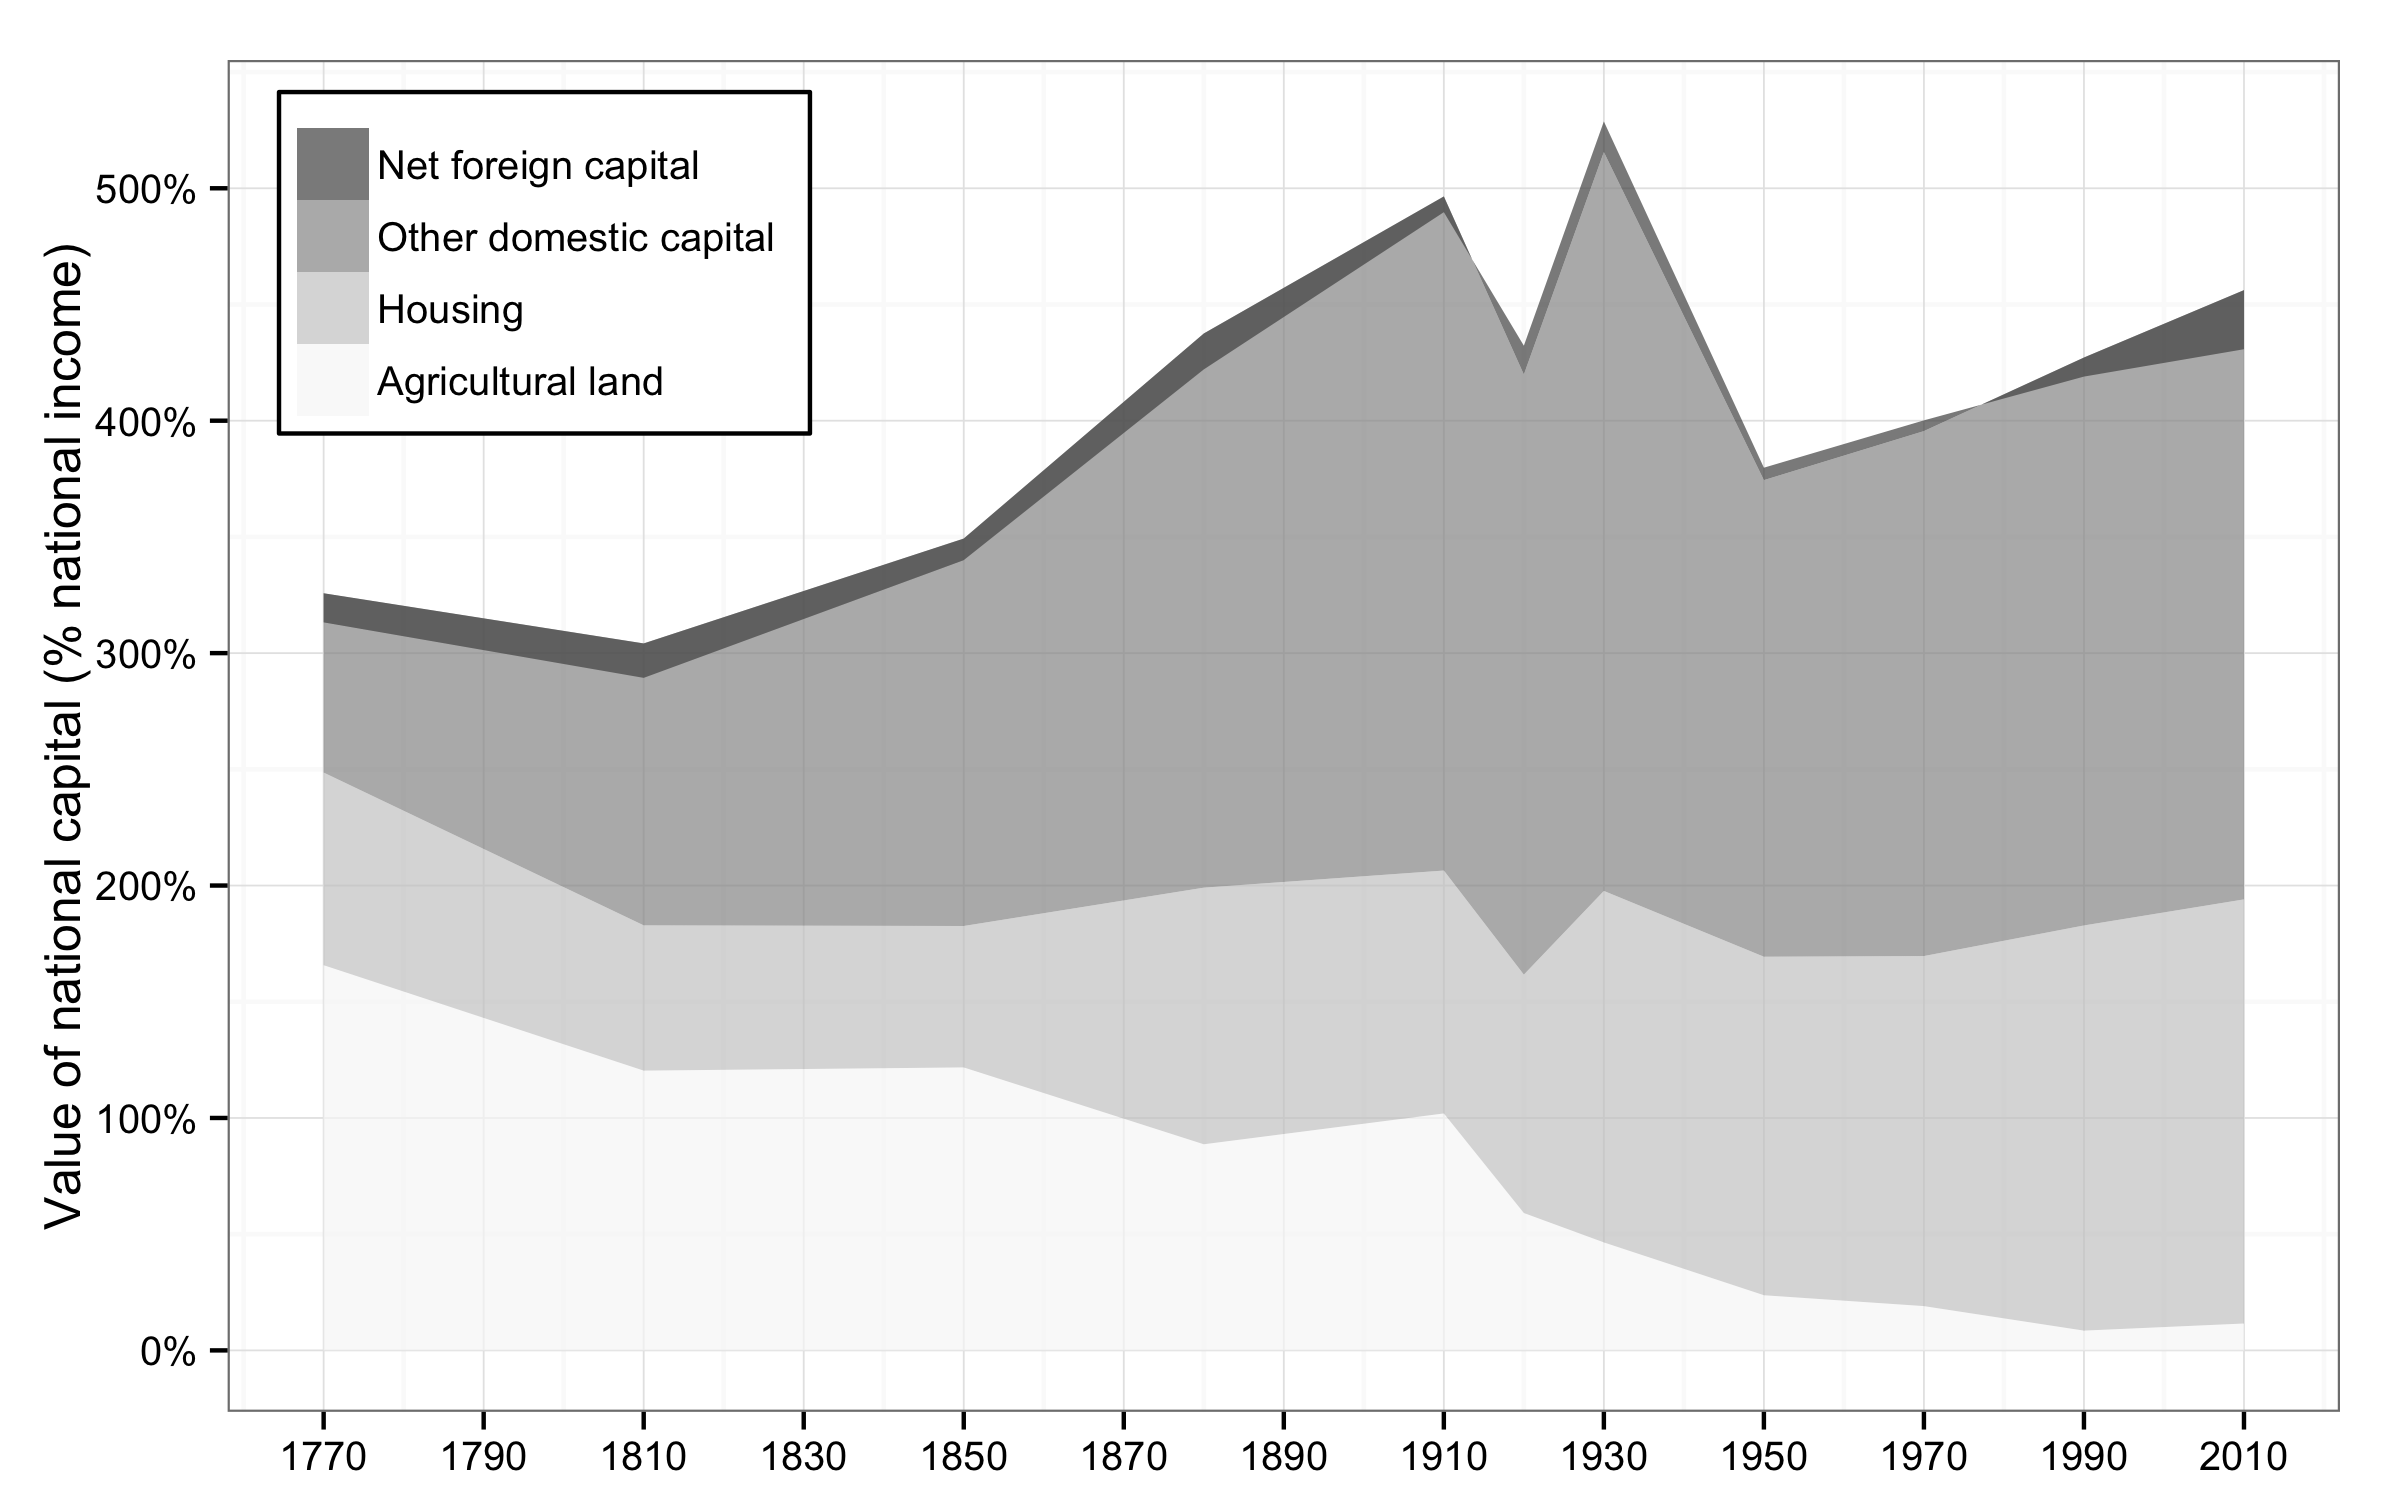
\includegraphics[width=1\linewidth]{figures/bw/Figure_4_6} 

}



\end{knitrout}
\caption{National capital is worth three years of national income in the United States in 1770 (including 1.5 years in agricultural land).}
\end{minipage}
\end{figure}
\end{frame}
%%%%%%%%%%%%%%%%%%%% Frame Here %%%%%%%%%%%%%%%%%%%%%%%%%%%%%%%%%%%%%%%%%%%%%%%%


%%%%%%%%%%%%%%%%%%%% Frame Here %%%%%%%%%%%%%%%%%%%%%%%%%%%%%%%%%%%%%%%%%%%%%%%%
\begin{frame}[label=Figure_4_7]
\frametitle{Figure 4.7. Public wealth in the United States, 1770--2010}
\begin{figure}[t]
\begin{minipage}[b]{\textwidth}
\centering
\begin{knitrout}\footnotesize
\definecolor{shadecolor}{rgb}{0.969, 0.969, 0.969}\color{fgcolor}

{\centering 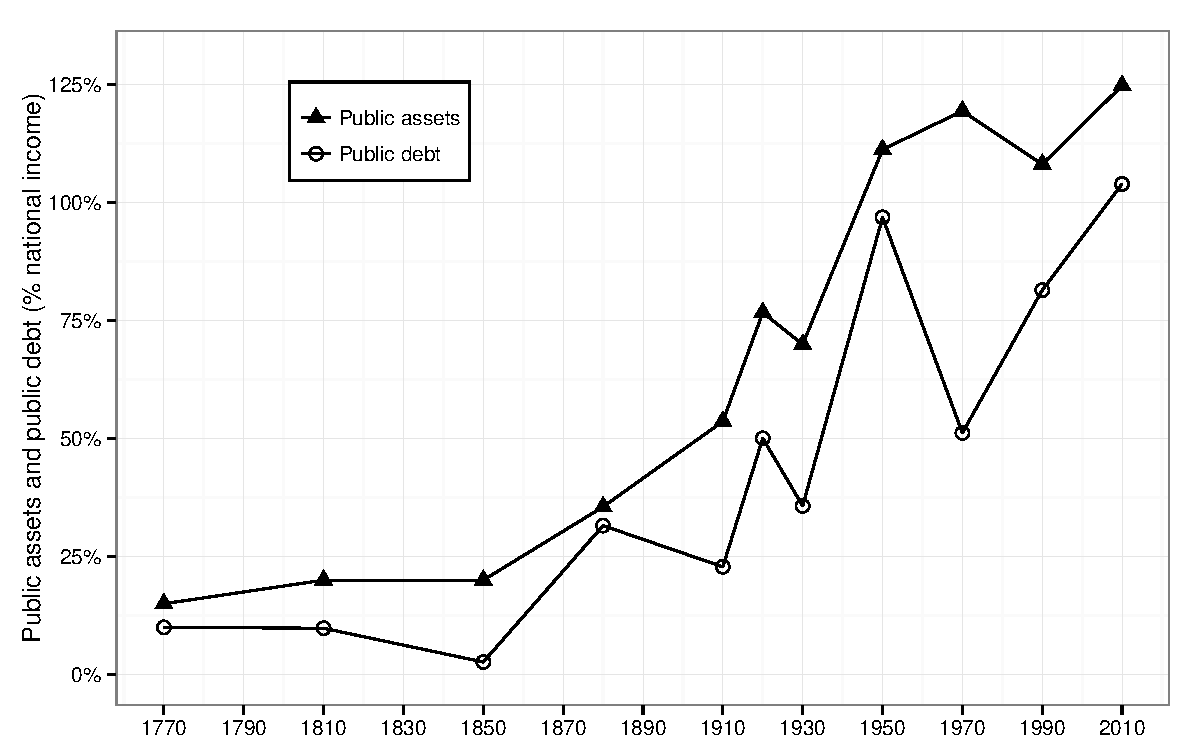
\includegraphics[width=1\linewidth]{figures/bw/Figure_4_7} 

}



\end{knitrout}
\caption{Public debt is worth one year of national income in the United States in 1950 (almost as much as assets).}
\end{minipage}
\end{figure}
\end{frame}
%%%%%%%%%%%%%%%%%%%% Frame Here %%%%%%%%%%%%%%%%%%%%%%%%%%%%%%%%%%%%%%%%%%%%%%%%


%%%%%%%%%%%%%%%%%%%% Frame Here %%%%%%%%%%%%%%%%%%%%%%%%%%%%%%%%%%%%%%%%%%%%%%%%
\begin{frame}[label=Figure_4_8]
\frametitle{Figure 4.8. Private and public capital in the United States, 1770--2010}
\begin{figure}[t]
\begin{minipage}[b]{\textwidth}
\centering
\begin{knitrout}\footnotesize
\definecolor{shadecolor}{rgb}{0.969, 0.969, 0.969}\color{fgcolor}

{\centering 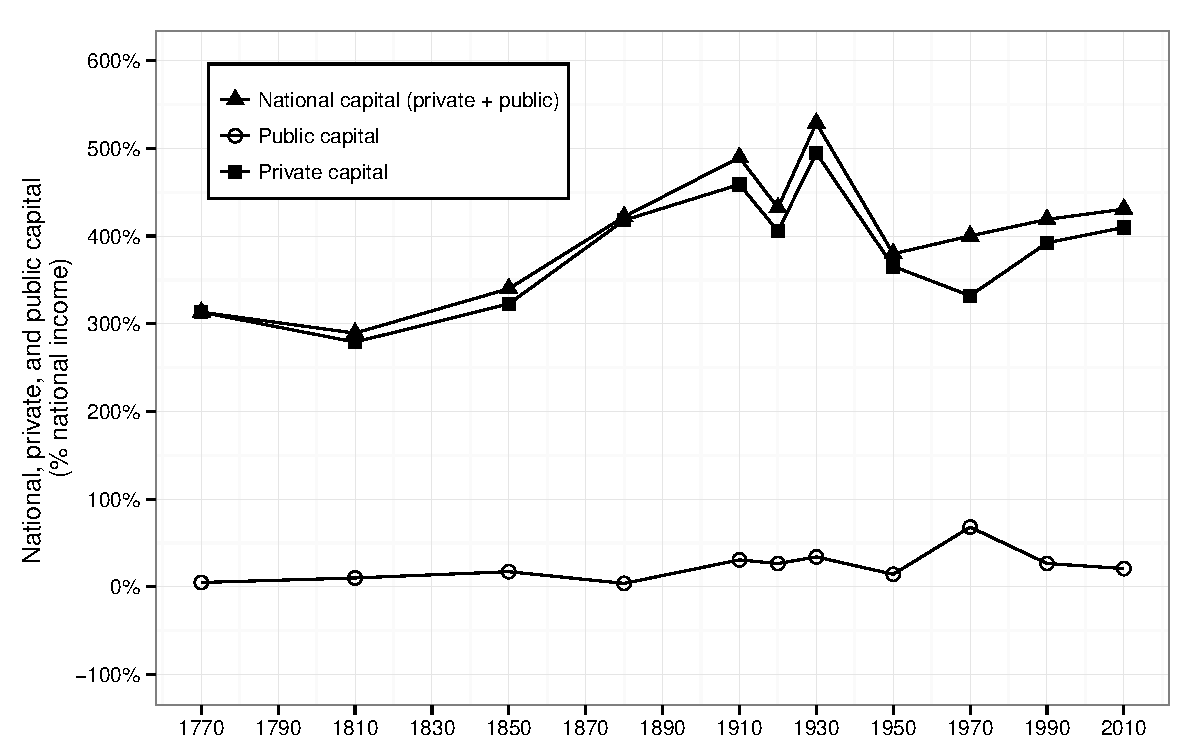
\includegraphics[width=1\linewidth]{figures/bw/Figure_4_8} 

}



\end{knitrout}
\caption{In 2010, public capital is worth 20 percent of national income, versus over 400 percent for private capital.}
\end{minipage}
\end{figure}
\end{frame}
%%%%%%%%%%%%%%%%%%%% Frame Here %%%%%%%%%%%%%%%%%%%%%%%%%%%%%%%%%%%%%%%%%%%%%%%%


%%%%%%%%%%%%%%%%%%%% Frame Here %%%%%%%%%%%%%%%%%%%%%%%%%%%%%%%%%%%%%%%%%%%%%%%%
\begin{frame}[label=Figure_4_9]
\frametitle{Figure 4.9. Capital in Canada, 1860--2010}
\begin{figure}[t]
\begin{minipage}[b]{\textwidth}
\centering
\begin{knitrout}\footnotesize
\definecolor{shadecolor}{rgb}{0.969, 0.969, 0.969}\color{fgcolor}

{\centering 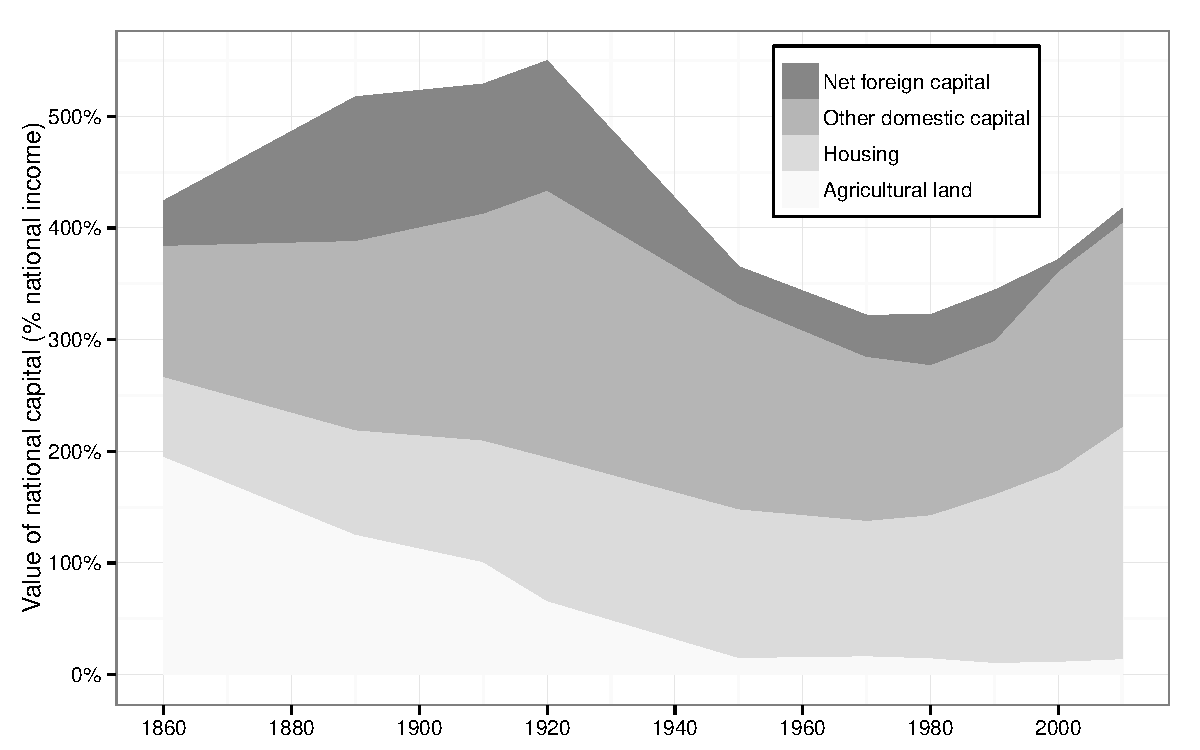
\includegraphics[width=1\linewidth]{figures/bw/Figure_4_9} 

}



\end{knitrout}
\caption{In Canada, a substantial part of domestic capital has always been held by the rest of the world, so that national capital has always been less than domestic capital.}
\end{minipage}
\end{figure}
\end{frame}
%%%%%%%%%%%%%%%%%%%% Frame Here %%%%%%%%%%%%%%%%%%%%%%%%%%%%%%%%%%%%%%%%%%%%%%%%


%%%%%%%%%%%%%%%%%%%% Frame Here %%%%%%%%%%%%%%%%%%%%%%%%%%%%%%%%%%%%%%%%%%%%%%%%
\begin{frame}[label=Figure_4_10]
\frametitle{Figure 4.10. Capital and slavery in the United States}
\begin{figure}[t]
\begin{minipage}[b]{\textwidth}
\centering
\begin{knitrout}\footnotesize
\definecolor{shadecolor}{rgb}{0.969, 0.969, 0.969}\color{fgcolor}

{\centering 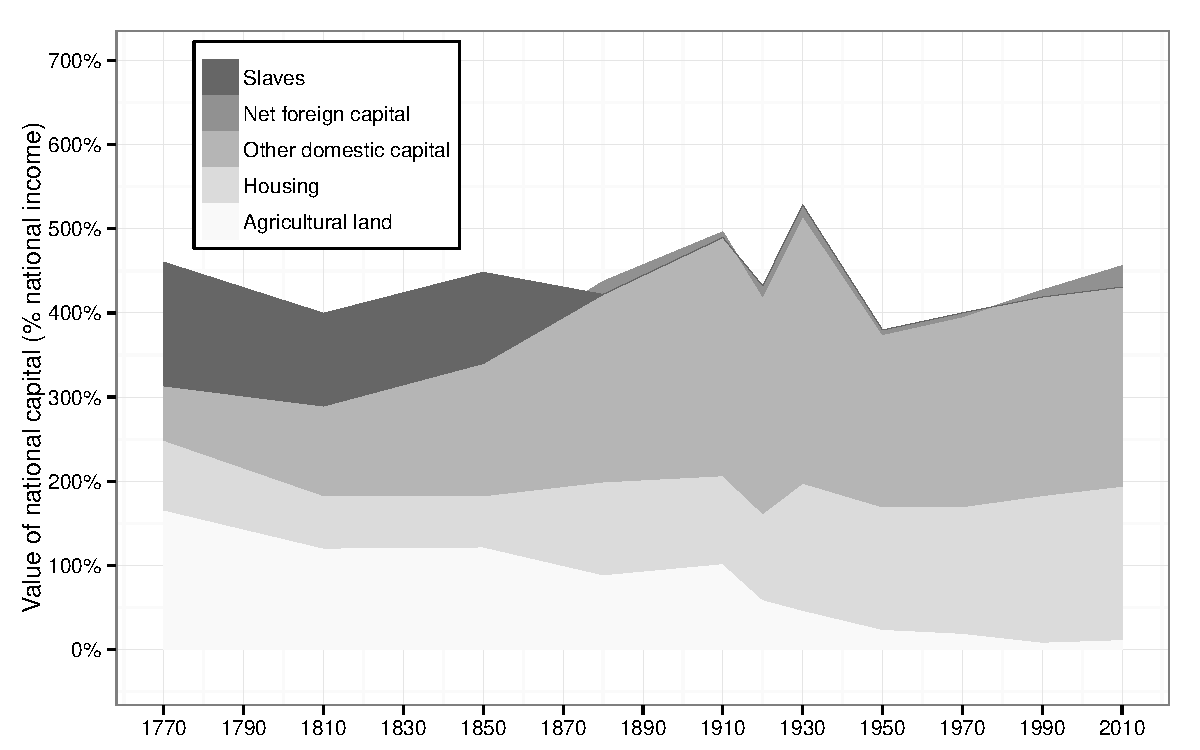
\includegraphics[width=1\linewidth]{figures/bw/Figure_4_10} 

}



\end{knitrout}
\caption{The market value of slaves was about 1.5 years of US national income around 1770 (as much as land).}
\end{minipage}
\end{figure}
\end{frame}
%%%%%%%%%%%%%%%%%%%% Frame Here %%%%%%%%%%%%%%%%%%%%%%%%%%%%%%%%%%%%%%%%%%%%%%%%


%%%%%%%%%%%%%%%%%%%% Frame Here %%%%%%%%%%%%%%%%%%%%%%%%%%%%%%%%%%%%%%%%%%%%%%%%
\begin{frame}[label=Figure_4_11]
\frametitle{Figure 4.11. Capital around 1770--1810: Old and New World}
\begin{figure}[t]
\begin{minipage}[b]{\textwidth}
\centering
\begin{knitrout}\footnotesize
\definecolor{shadecolor}{rgb}{0.969, 0.969, 0.969}\color{fgcolor}

{\centering 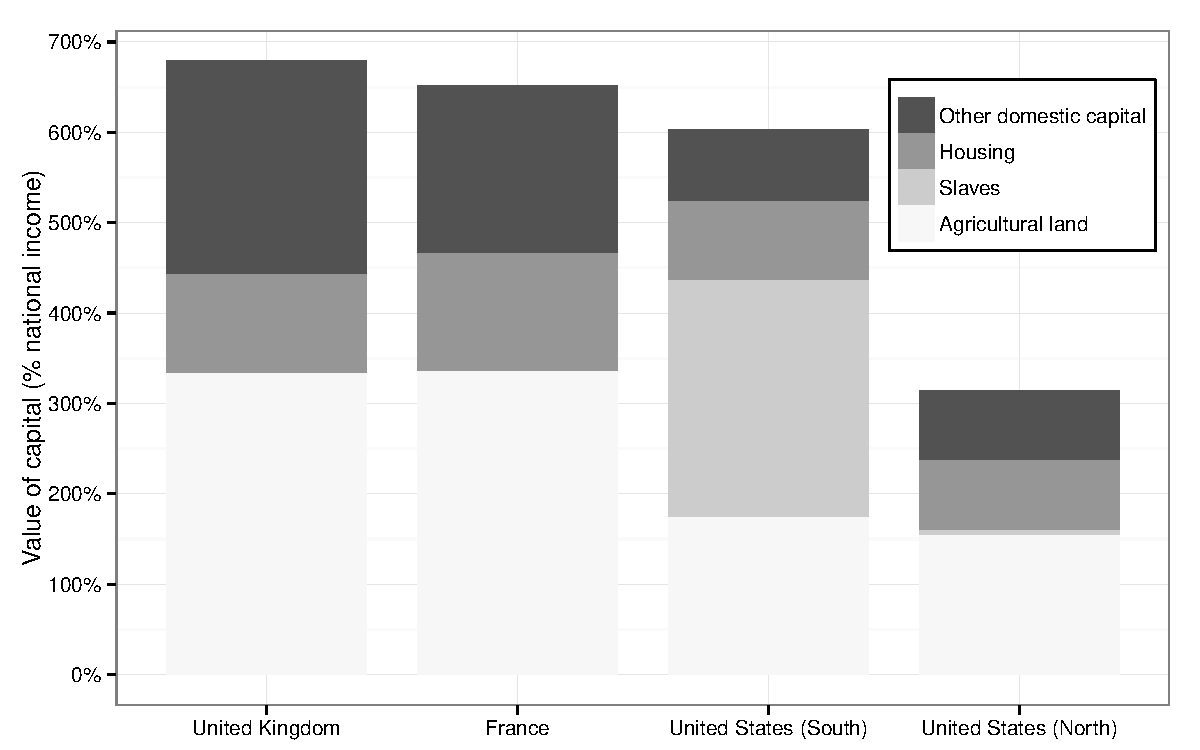
\includegraphics[width=1\linewidth]{figures/bw/Figure_4_11} 

}



\end{knitrout}
\caption{The combined value of agricultural land and slaves in the Southern United States surpassed four years of national income around 1770--1810.}
\end{minipage}
\end{figure}
\end{frame}
%%%%%%%%%%%%%%%%%%%% Frame Here %%%%%%%%%%%%%%%%%%%%%%%%%%%%%%%%%%%%%%%%%%%%%%%%


%%%%%%%%%%%%%%%%%%%% Frame Here %%%%%%%%%%%%%%%%%%%%%%%%%%%%%%%%%%%%%%%%%%%%%%%%
\begin{frame}[label=Figure_5_1]
\frametitle{Figure 5.1. Private \& public capital in Europe \& United States, 1870--2010}
\begin{figure}[t]
\begin{minipage}[b]{\textwidth}
\centering
\begin{knitrout}\footnotesize
\definecolor{shadecolor}{rgb}{0.969, 0.969, 0.969}\color{fgcolor}

{\centering 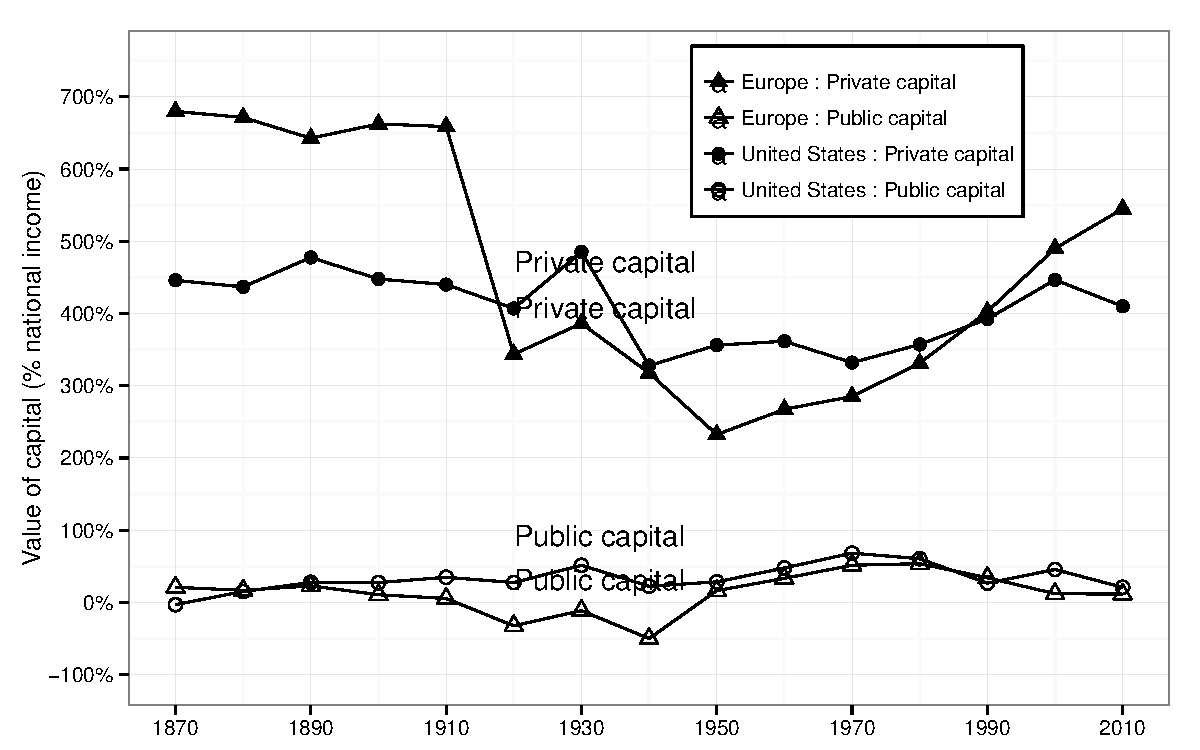
\includegraphics[width=1\linewidth]{figures/bw/Figure_5_1} 

}



\end{knitrout}
\caption{The fluctuations of national capital in the long run correspond mostly to the fluctuations of private capital (both in Europe and in the United States).}
\end{minipage}
\end{figure}
\end{frame}
%%%%%%%%%%%%%%%%%%%% Frame Here %%%%%%%%%%%%%%%%%%%%%%%%%%%%%%%%%%%%%%%%%%%%%%%%


%%%%%%%%%%%%%%%%%%%% Frame Here %%%%%%%%%%%%%%%%%%%%%%%%%%%%%%%%%%%%%%%%%%%%%%%%
\begin{frame}[label=Figure_5_2]
\frametitle{Figure 5.2. National capital in Europe \& United States, 1870--2010}
\begin{figure}[t]
\begin{minipage}[b]{\textwidth}
\centering
\begin{knitrout}\footnotesize
\definecolor{shadecolor}{rgb}{0.969, 0.969, 0.969}\color{fgcolor}

{\centering 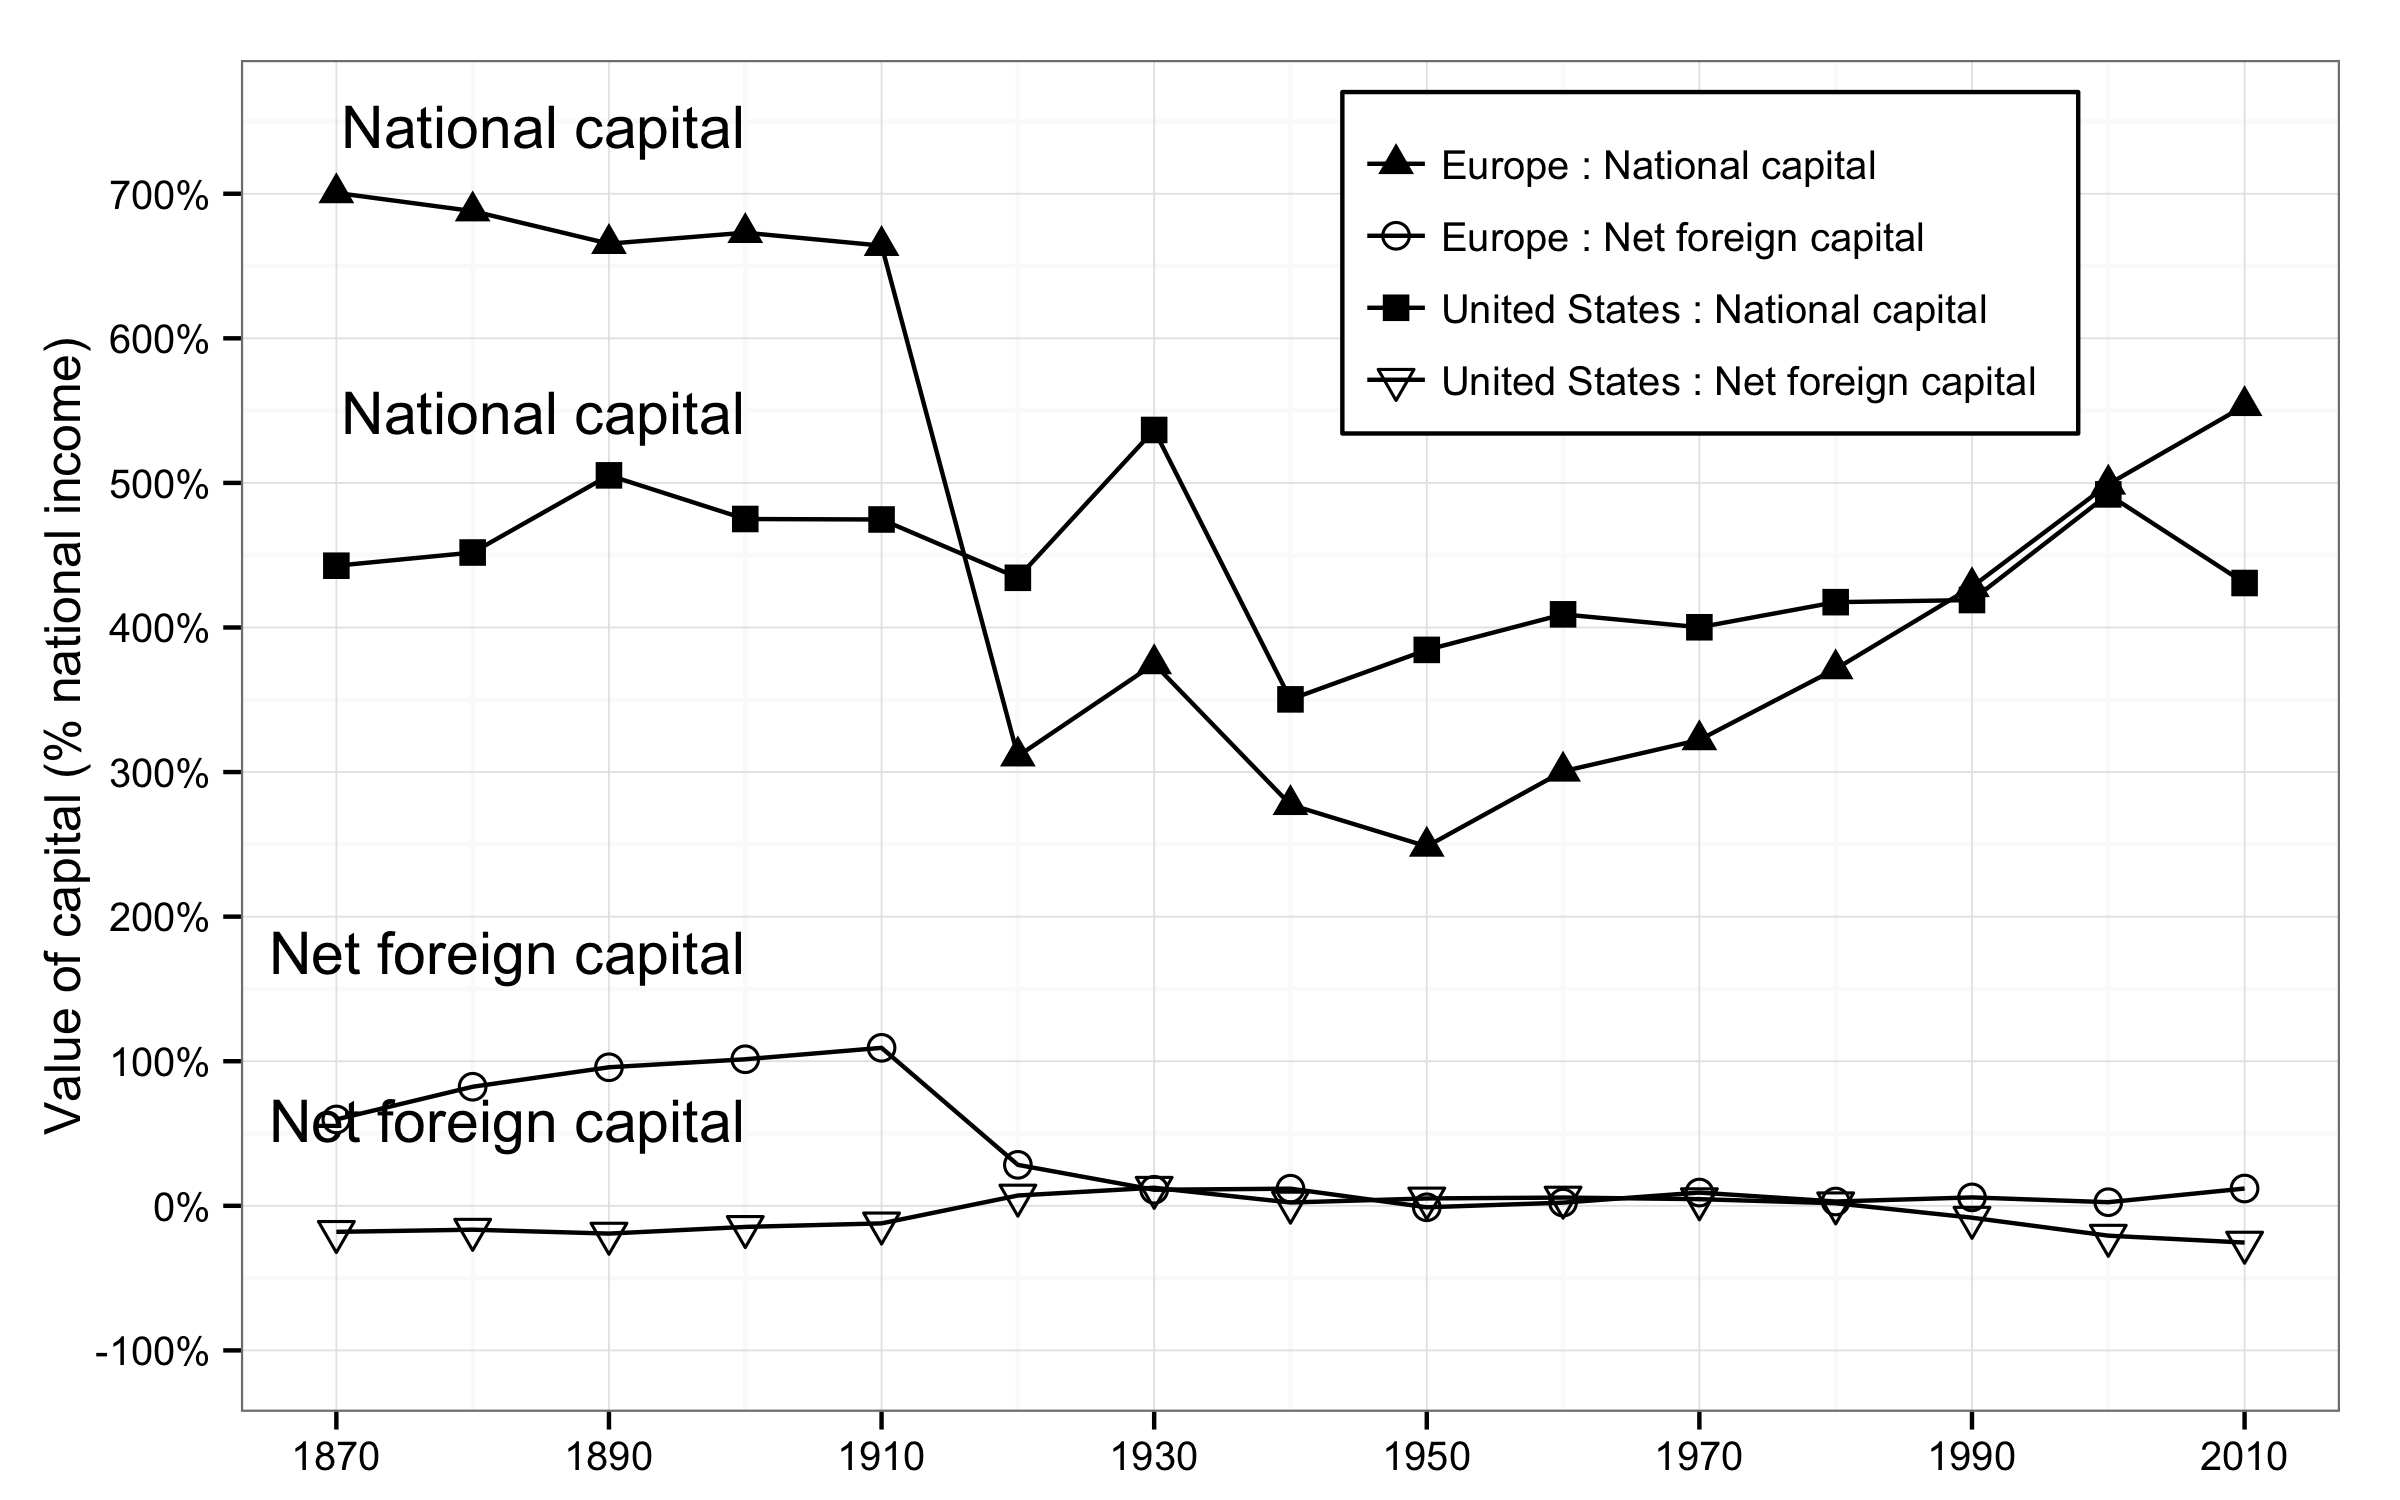
\includegraphics[width=1\linewidth]{figures/bw/Figure_5_2} 

}



\end{knitrout}
\caption{National capital (public and private) is worth 6.5 years of national income in Europe in 1910, versus 4.5 years in the United States.}
\end{minipage}
\end{figure}
\end{frame}
%%%%%%%%%%%%%%%%%%%% Frame Here %%%%%%%%%%%%%%%%%%%%%%%%%%%%%%%%%%%%%%%%%%%%%%%%


%%%%%%%%%%%%%%%%%%%% Frame Here %%%%%%%%%%%%%%%%%%%%%%%%%%%%%%%%%%%%%%%%%%%%%%%%
\begin{frame}[label=Figure_5_3]
\frametitle{Figure 5.3. Private capital in rich countries, 1970--2010}
\begin{figure}[t]
\begin{minipage}[b]{\textwidth}
\centering
\begin{knitrout}\footnotesize
\definecolor{shadecolor}{rgb}{0.969, 0.969, 0.969}\color{fgcolor}

{\centering 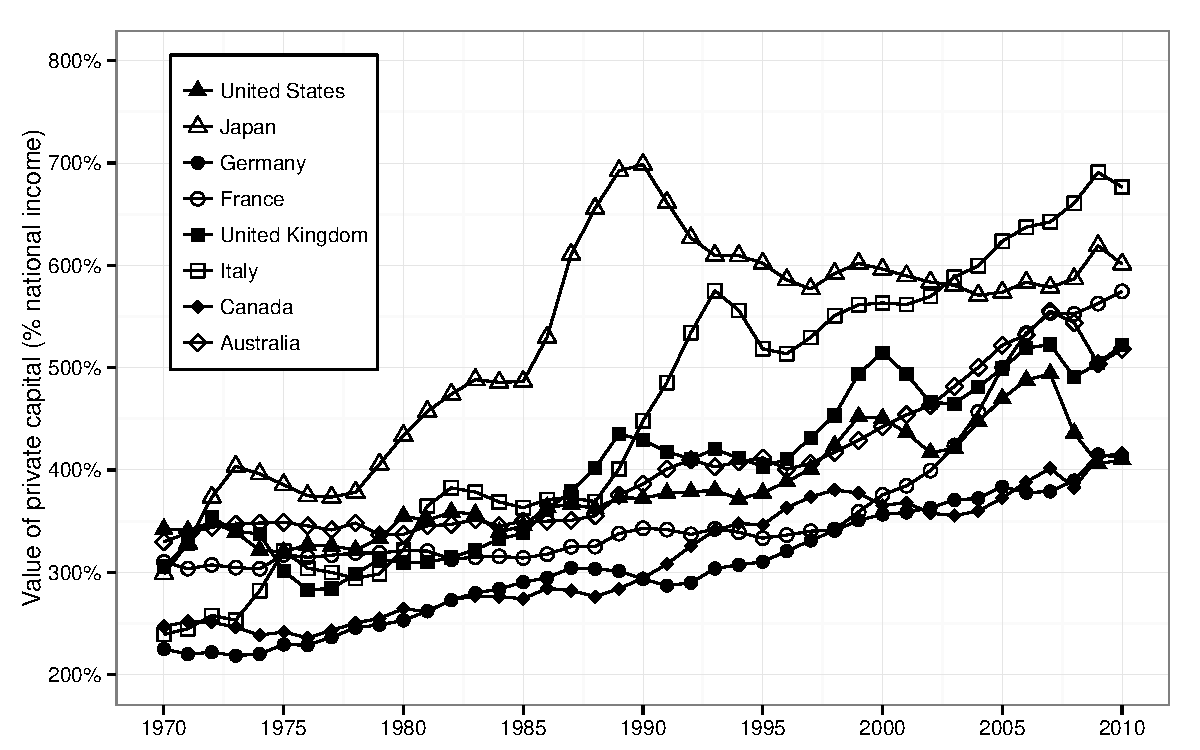
\includegraphics[width=1\linewidth]{figures/bw/Figure_5_3} 

}



\end{knitrout}
\caption{Private capital is worth between 2 and 3.5 years of national income in rich countries in 1970, and between 4 and 7 years of national income in 2010.}
\end{minipage}
\end{figure}
\end{frame}
%%%%%%%%%%%%%%%%%%%% Frame Here %%%%%%%%%%%%%%%%%%%%%%%%%%%%%%%%%%%%%%%%%%%%%%%%


%%%%%%%%%%%%%%%%%%%% Frame Here %%%%%%%%%%%%%%%%%%%%%%%%%%%%%%%%%%%%%%%%%%%%%%%%
\begin{frame}[label=Figure_5_3S]
\frametitle{Figure 5.3S. Private capital in rich countries, 1970--2010}
\begin{figure}[t]
\begin{minipage}[b]{\textwidth}
\centering
\begin{knitrout}\footnotesize
\definecolor{shadecolor}{rgb}{0.969, 0.969, 0.969}\color{fgcolor}

{\centering 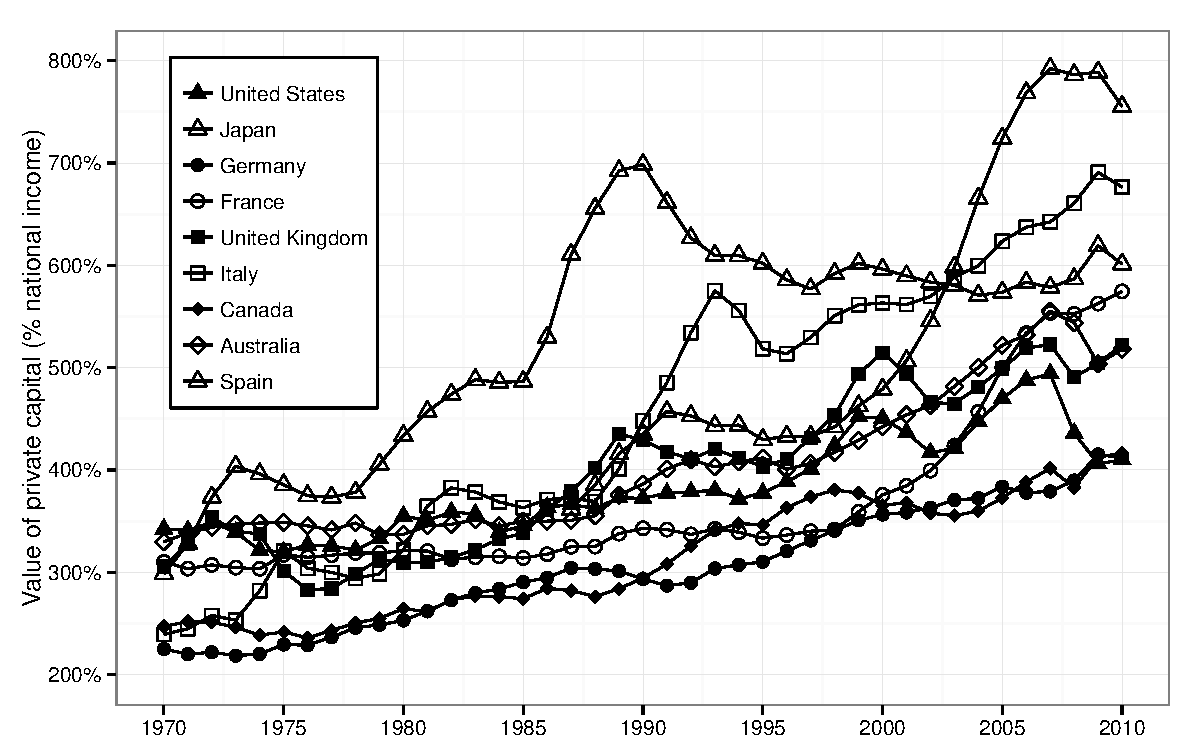
\includegraphics[width=1\linewidth]{figures/bw/Figure_5_3S} 

}



\end{knitrout}
\caption{Private capital is worth between 2 and 3.5 years of national income in rich countries in 1970, and between 4 and 7 years of national income in 2010.}
\end{minipage}
\end{figure}
\end{frame}
%%%%%%%%%%%%%%%%%%%% Frame Here %%%%%%%%%%%%%%%%%%%%%%%%%%%%%%%%%%%%%%%%%%%%%%%%


%%%%%%%%%%%%%%%%%%%% Frame Here %%%%%%%%%%%%%%%%%%%%%%%%%%%%%%%%%%%%%%%%%%%%%%%%
\begin{frame}[label=Figure_5_4]
\frametitle{Figure 5.4. Private capital measured in years of disposable income, 1970--2010}
\begin{figure}[t]
\begin{minipage}[b]{\textwidth}
\centering
\begin{knitrout}\footnotesize
\definecolor{shadecolor}{rgb}{0.969, 0.969, 0.969}\color{fgcolor}

{\centering 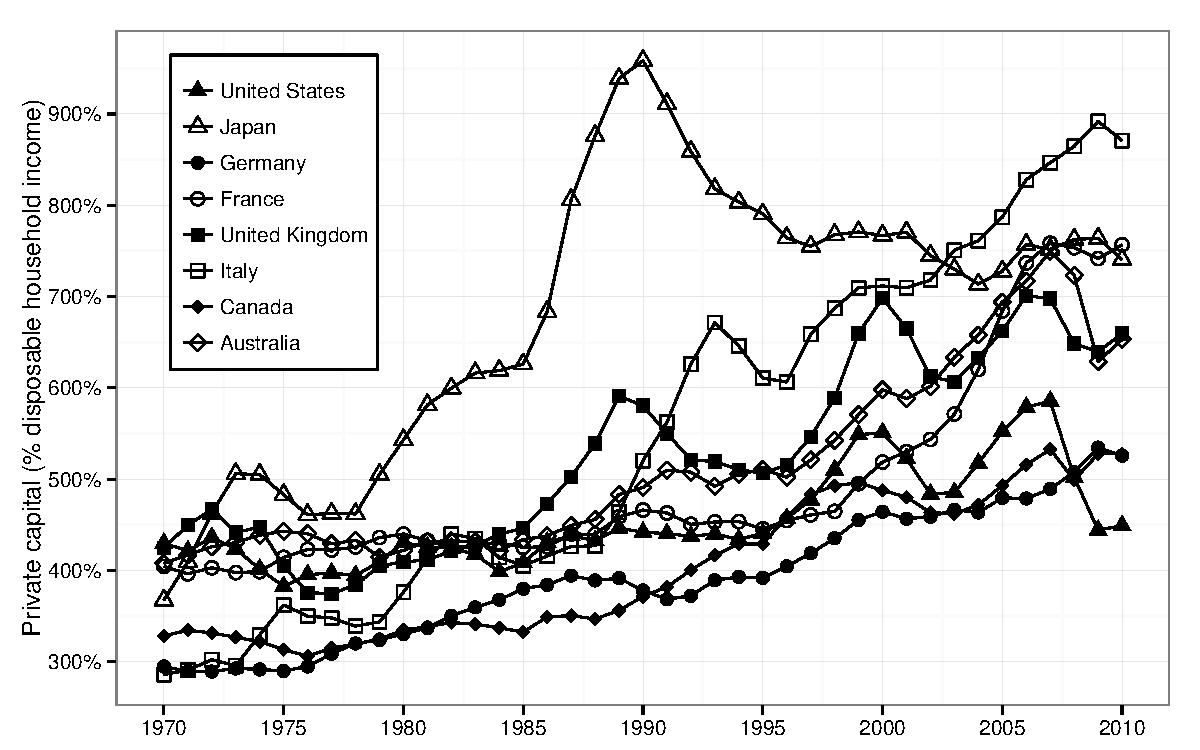
\includegraphics[width=1\linewidth]{figures/bw/Figure_5_4} 

}



\end{knitrout}
\caption{Expressed in years of household disposable income (about 70--80\% of national income), the capital/income ratio appears to be larger than when it is expressed in years of national income.}
\end{minipage}
\end{figure}
\end{frame}
%%%%%%%%%%%%%%%%%%%% Frame Here %%%%%%%%%%%%%%%%%%%%%%%%%%%%%%%%%%%%%%%%%%%%%%%%


%%%%%%%%%%%%%%%%%%%% Frame Here %%%%%%%%%%%%%%%%%%%%%%%%%%%%%%%%%%%%%%%%%%%%%%%%
\begin{frame}[label=Figure_5_4S]
\frametitle{Figure 5.4S. Private capital measured in years of disposable income, 1970--2010}
\begin{figure}[t]
\begin{minipage}[b]{\textwidth}
\centering
\begin{knitrout}\footnotesize
\definecolor{shadecolor}{rgb}{0.969, 0.969, 0.969}\color{fgcolor}

{\centering 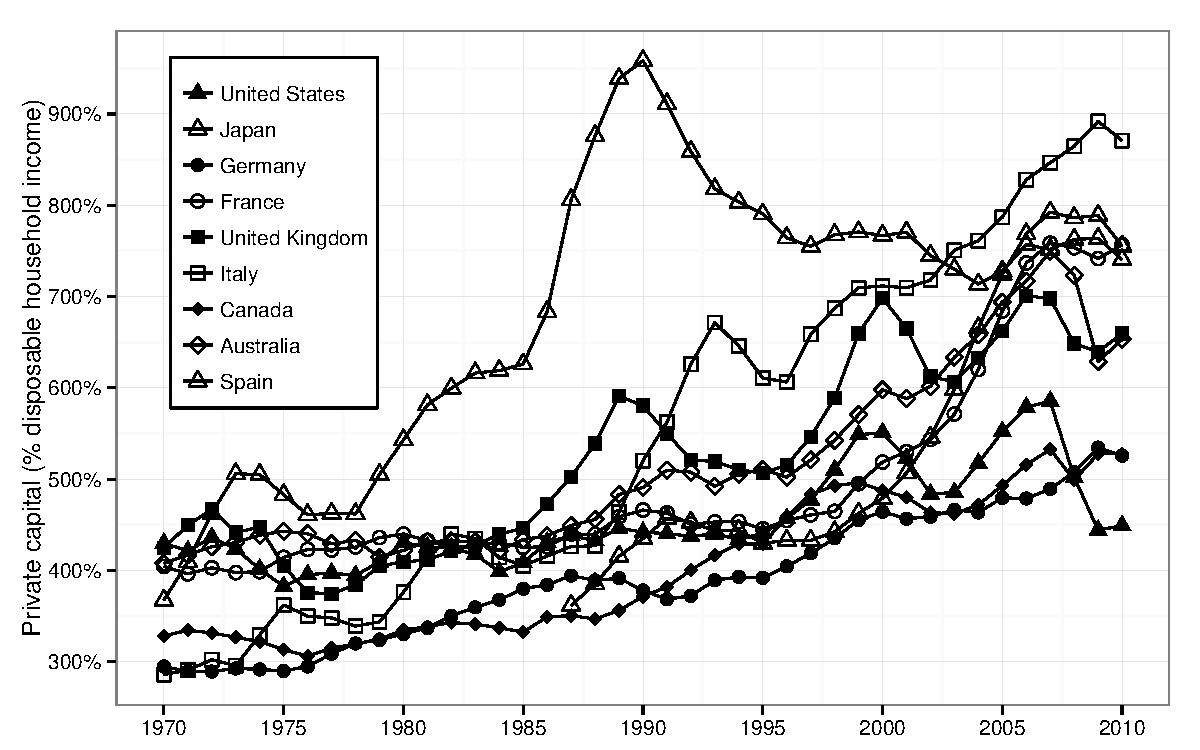
\includegraphics[width=1\linewidth]{figures/bw/Figure_5_4S} 

}



\end{knitrout}
\caption{Expressed in years of household disposable income (about 70--80\% of national income), the capital/income ratio appears to be larger than when it is expressed in years of national income.}
\end{minipage}
\end{figure}
\end{frame}
%%%%%%%%%%%%%%%%%%%% Frame Here %%%%%%%%%%%%%%%%%%%%%%%%%%%%%%%%%%%%%%%%%%%%%%%%


%%%%%%%%%%%%%%%%%%%% Frame Here %%%%%%%%%%%%%%%%%%%%%%%%%%%%%%%%%%%%%%%%%%%%%%%%
\begin{frame}[label=Figure_5_5X]
\frametitle{Figure 5.5X. Public capital in rich countries, 1970--2010}
\begin{figure}[t]
\begin{minipage}[b]{\textwidth}
\centering
\begin{knitrout}\footnotesize
\definecolor{shadecolor}{rgb}{0.969, 0.969, 0.969}\color{fgcolor}

{\centering 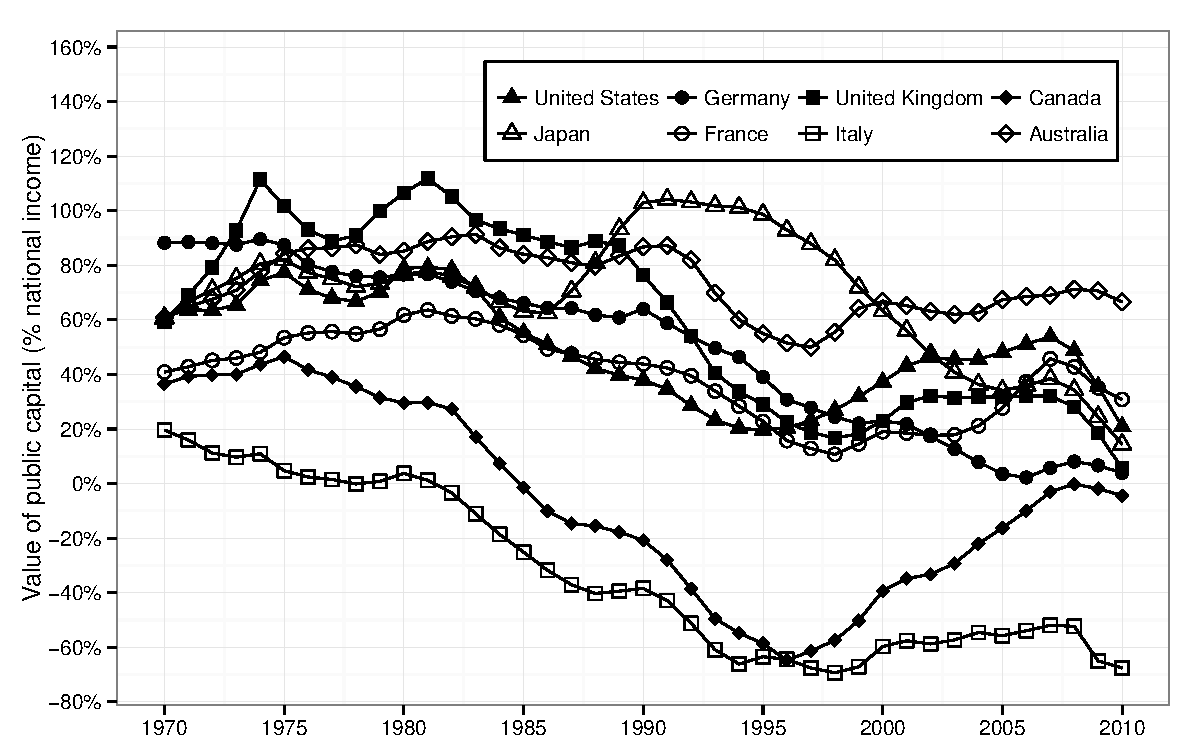
\includegraphics[width=1\linewidth]{figures/bw/Figure_5_5X} 

}



\end{knitrout}
\caption{In France, Britain, Germany, and the United States, government deficits exceeded public investment by 2--3\% of national income on average over the period 1970--2010, compared with more than 6\% in Italy.}
\end{minipage}
\end{figure}
\end{frame}
%%%%%%%%%%%%%%%%%%%% Frame Here %%%%%%%%%%%%%%%%%%%%%%%%%%%%%%%%%%%%%%%%%%%%%%%%


%%%%%%%%%%%%%%%%%%%% Frame Here %%%%%%%%%%%%%%%%%%%%%%%%%%%%%%%%%%%%%%%%%%%%%%%%
\begin{frame}[label=Figure_5_5XS]
\frametitle{Figure 5.5XS. Public capital in rich countries, 1970--2010}
\begin{figure}[t]
\begin{minipage}[b]{\textwidth}
\centering
\begin{knitrout}\footnotesize
\definecolor{shadecolor}{rgb}{0.969, 0.969, 0.969}\color{fgcolor}

{\centering 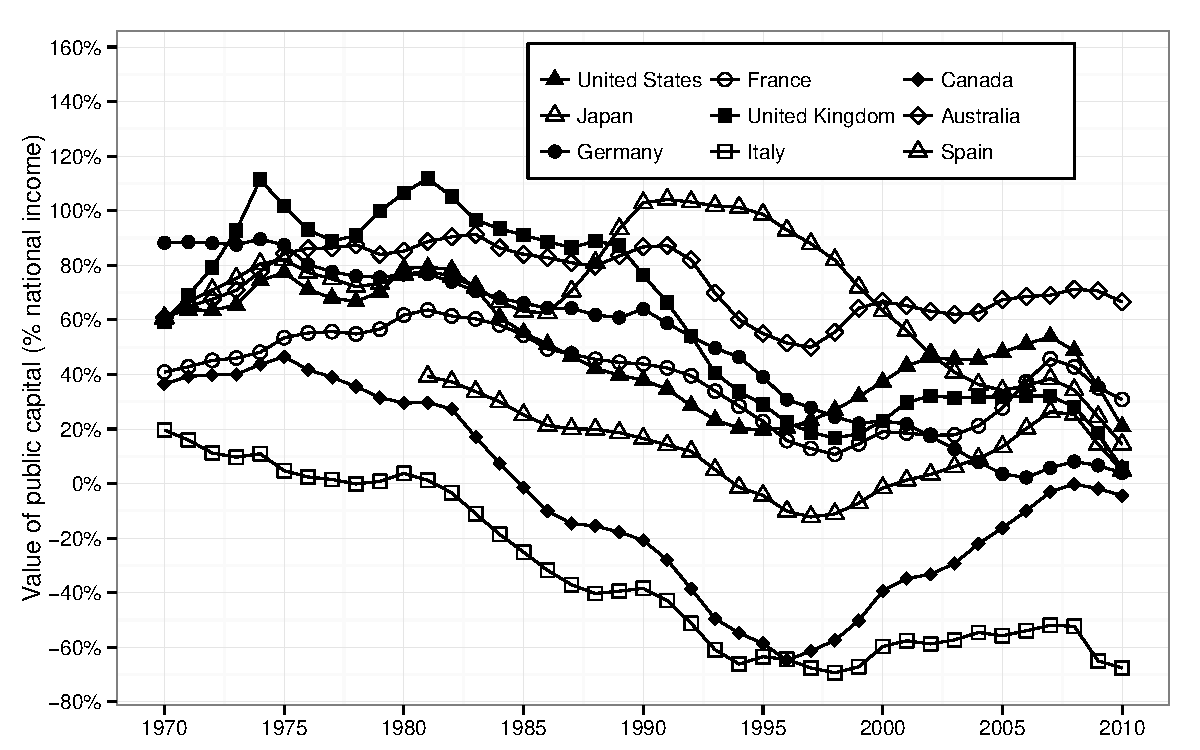
\includegraphics[width=1\linewidth]{figures/bw/Figure_5_5XS} 

}



\end{knitrout}
\caption{In France, Britain, Germany, and the United States, government deficits exceeded public investment by 2--3\% of national income on average over the period 1970--2010, compared with more than 6\% in Italy.}
\end{minipage}
\end{figure}
\end{frame}
%%%%%%%%%%%%%%%%%%%% Frame Here %%%%%%%%%%%%%%%%%%%%%%%%%%%%%%%%%%%%%%%%%%%%%%%%


%%%%%%%%%%%%%%%%%%%% Frame Here %%%%%%%%%%%%%%%%%%%%%%%%%%%%%%%%%%%%%%%%%%%%%%%%
\begin{frame}[label=Figure_5_5]
\frametitle{Figure 5.5. Private and public capital in rich countries, 1970--2010}
\begin{figure}[t]
\begin{minipage}[b]{\textwidth}
\centering
\begin{knitrout}\footnotesize
\definecolor{shadecolor}{rgb}{0.969, 0.969, 0.969}\color{fgcolor}

{\centering 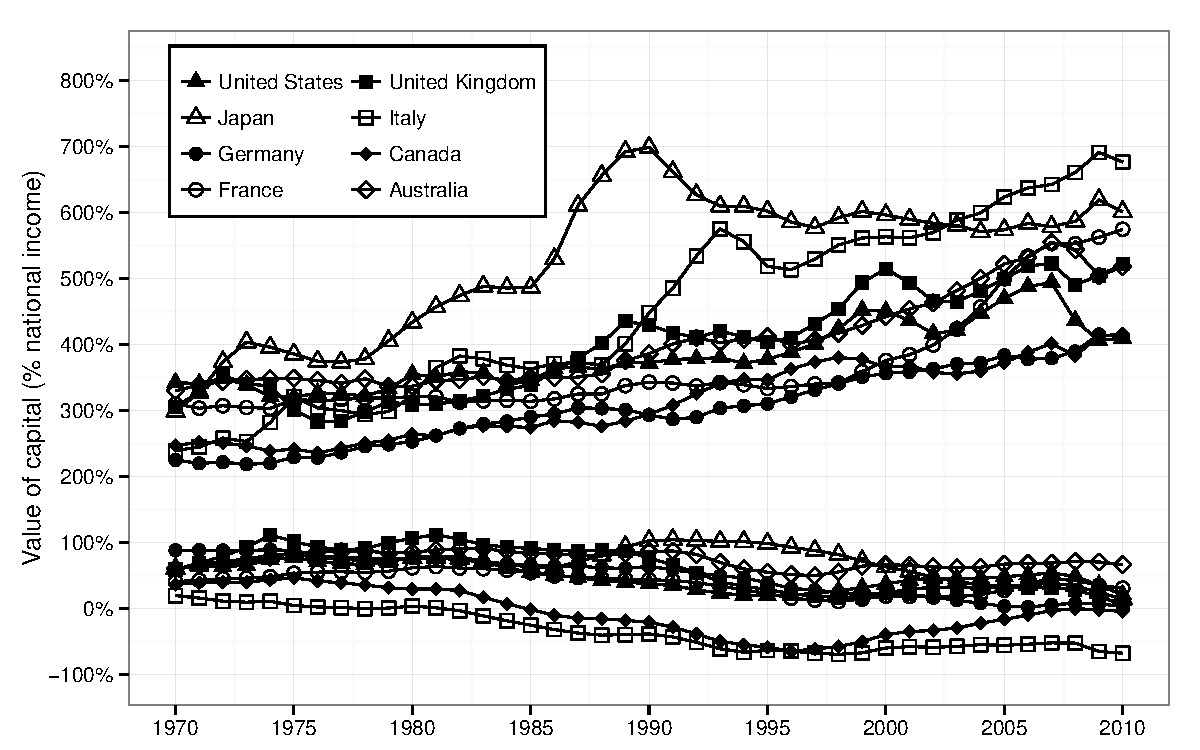
\includegraphics[width=1\linewidth]{figures/bw/Figure_5_5} 

}



\end{knitrout}
\caption{In Italy, private capital rose from 240\% to 680\% in national income between 1970 and 2010, while public capital dropped from 20\% to -70\%.}
\end{minipage}
\end{figure}
\end{frame}
%%%%%%%%%%%%%%%%%%%% Frame Here %%%%%%%%%%%%%%%%%%%%%%%%%%%%%%%%%%%%%%%%%%%%%%%%


%%%%%%%%%%%%%%%%%%%% Frame Here %%%%%%%%%%%%%%%%%%%%%%%%%%%%%%%%%%%%%%%%%%%%%%%%
\begin{frame}[label=Figure_5_6]
\frametitle{Figure 5.6. Market value and book value of corporations, 1970--2010}
\begin{figure}[t]
\begin{minipage}[b]{\textwidth}
\centering
\begin{knitrout}\footnotesize
\definecolor{shadecolor}{rgb}{0.969, 0.969, 0.969}\color{fgcolor}

{\centering 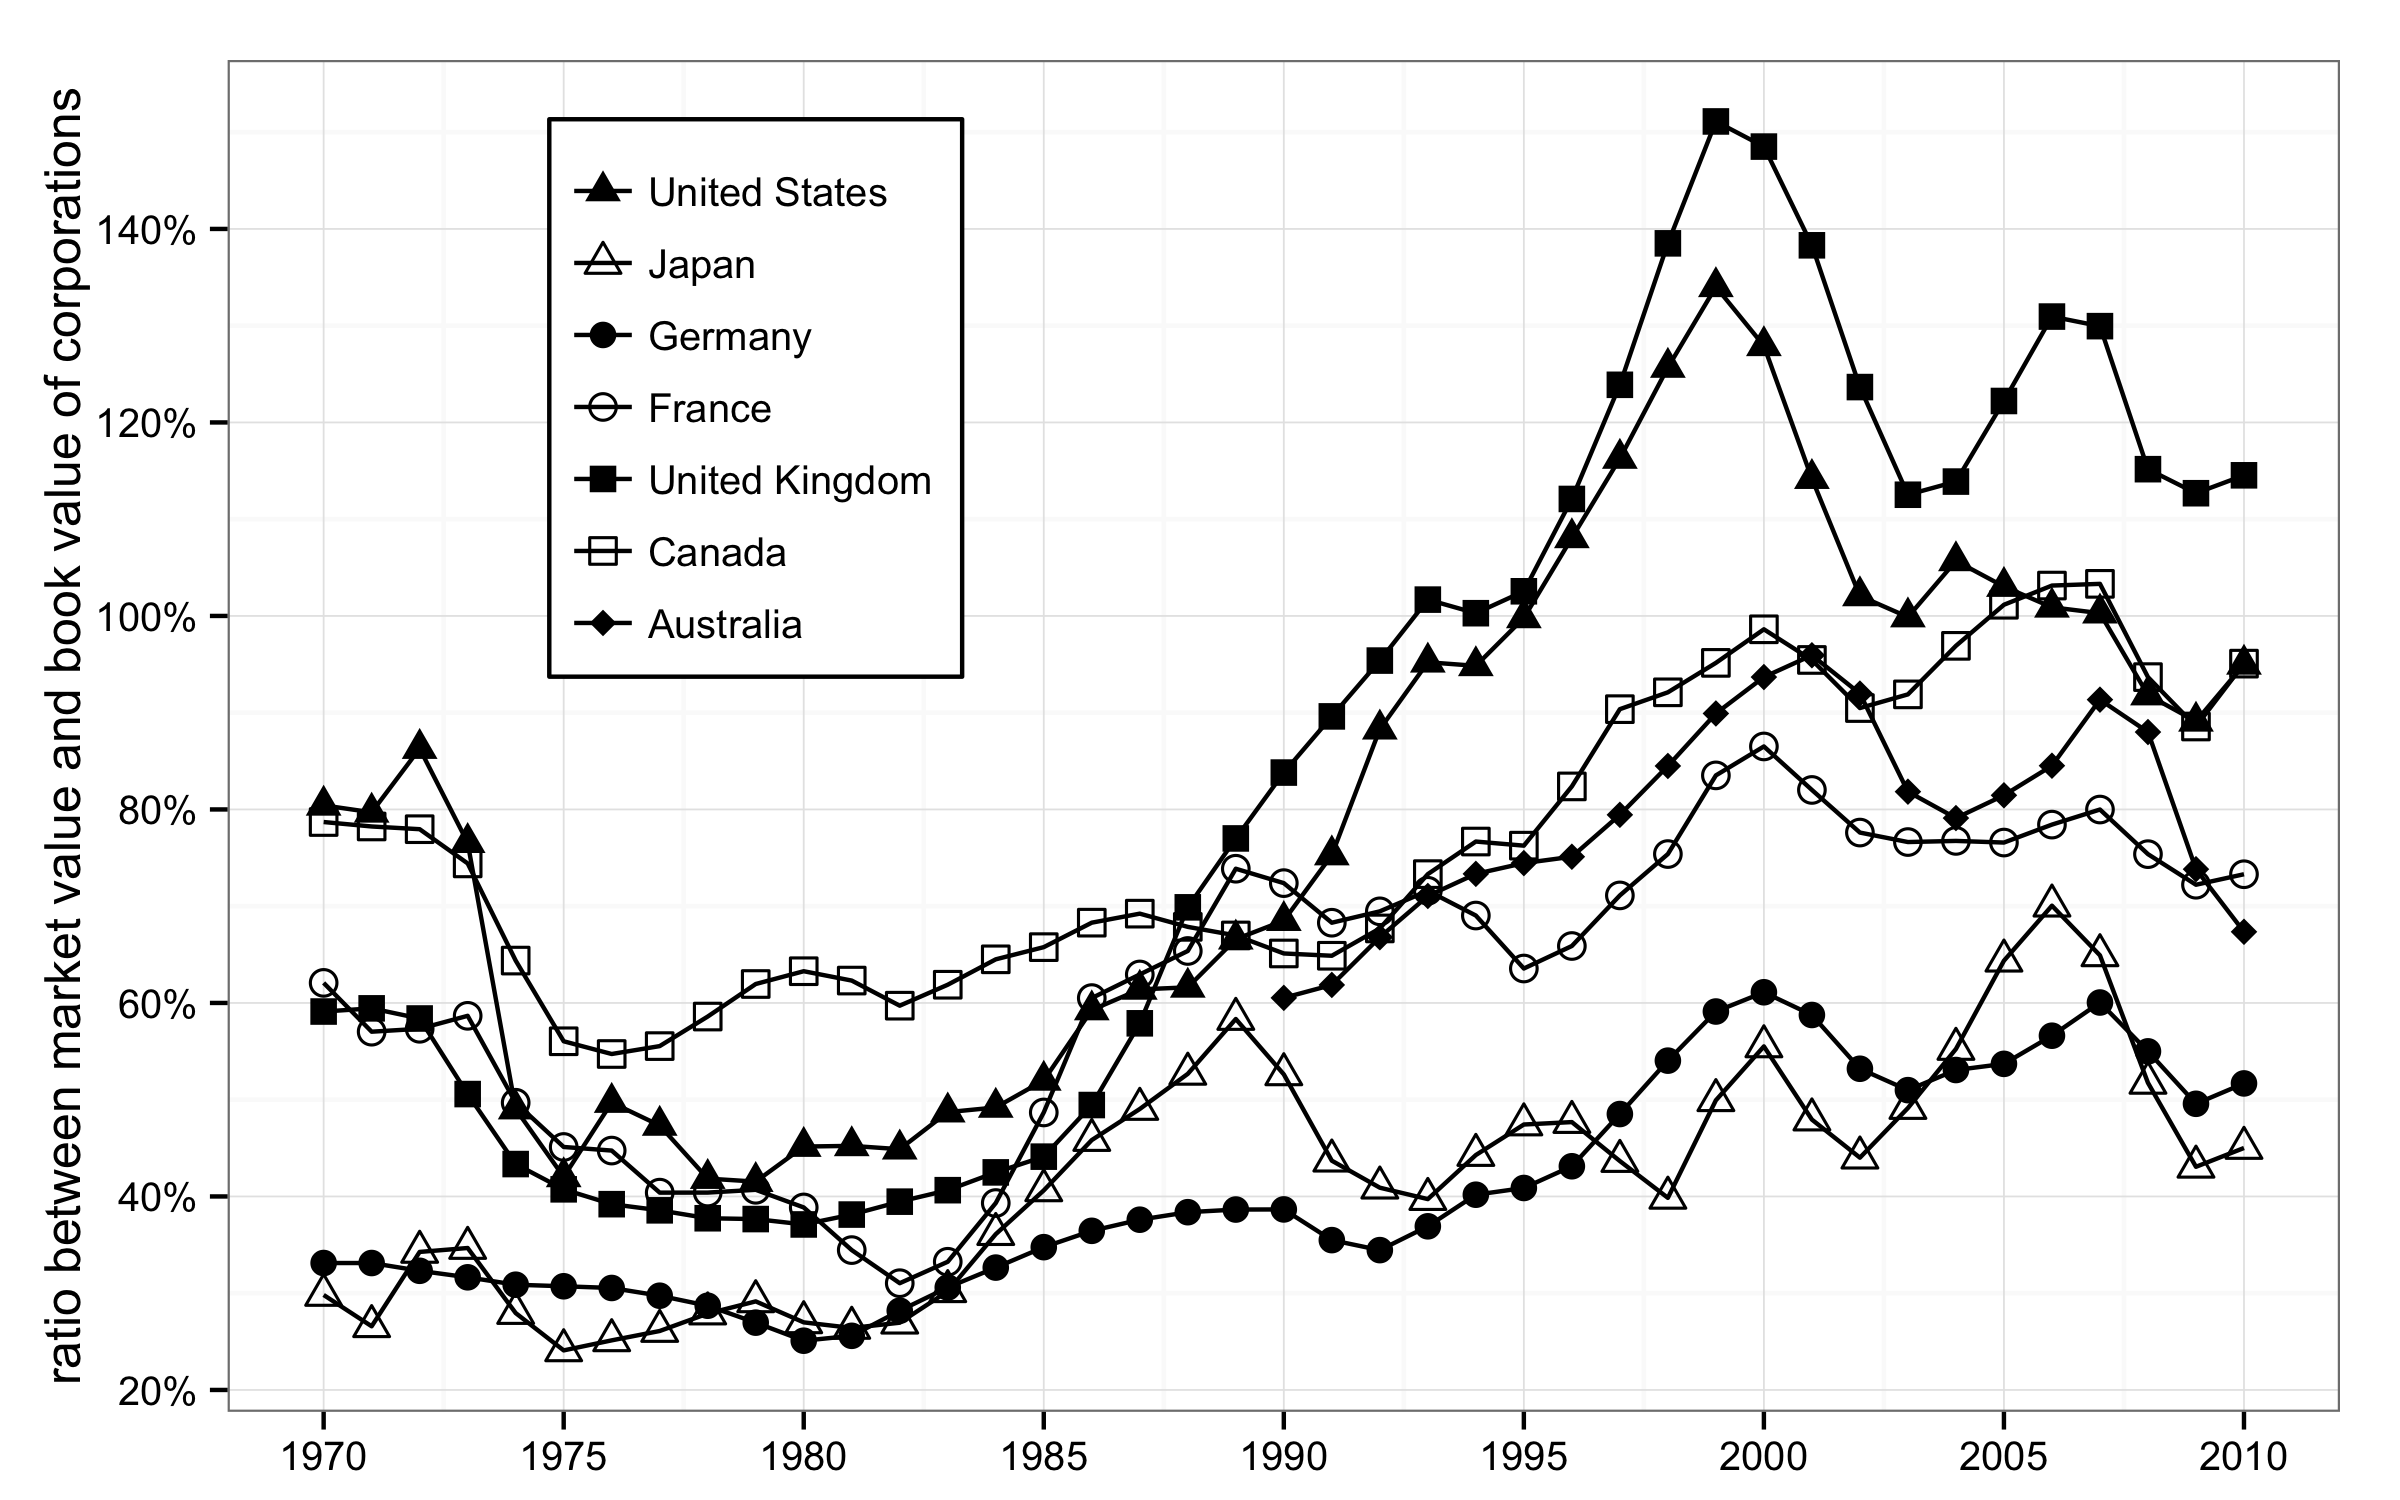
\includegraphics[width=1\linewidth]{figures/bw/Figure_5_6} 

}



\end{knitrout}
\caption{Tobin's Q (i.e. the ratio between market value and book value of corporations) has risen in rich countries since the 1970s--1980s.}
\end{minipage}
\end{figure}
\end{frame}
%%%%%%%%%%%%%%%%%%%% Frame Here %%%%%%%%%%%%%%%%%%%%%%%%%%%%%%%%%%%%%%%%%%%%%%%%


%%%%%%%%%%%%%%%%%%%% Frame Here %%%%%%%%%%%%%%%%%%%%%%%%%%%%%%%%%%%%%%%%%%%%%%%%
\begin{frame}[label=Figure_5_7]
\frametitle{Figure 5.7. National capital in rich countries, 1970--2010}
\begin{figure}[t]
\begin{minipage}[b]{\textwidth}
\centering
\begin{knitrout}\footnotesize
\definecolor{shadecolor}{rgb}{0.969, 0.969, 0.969}\color{fgcolor}

{\centering 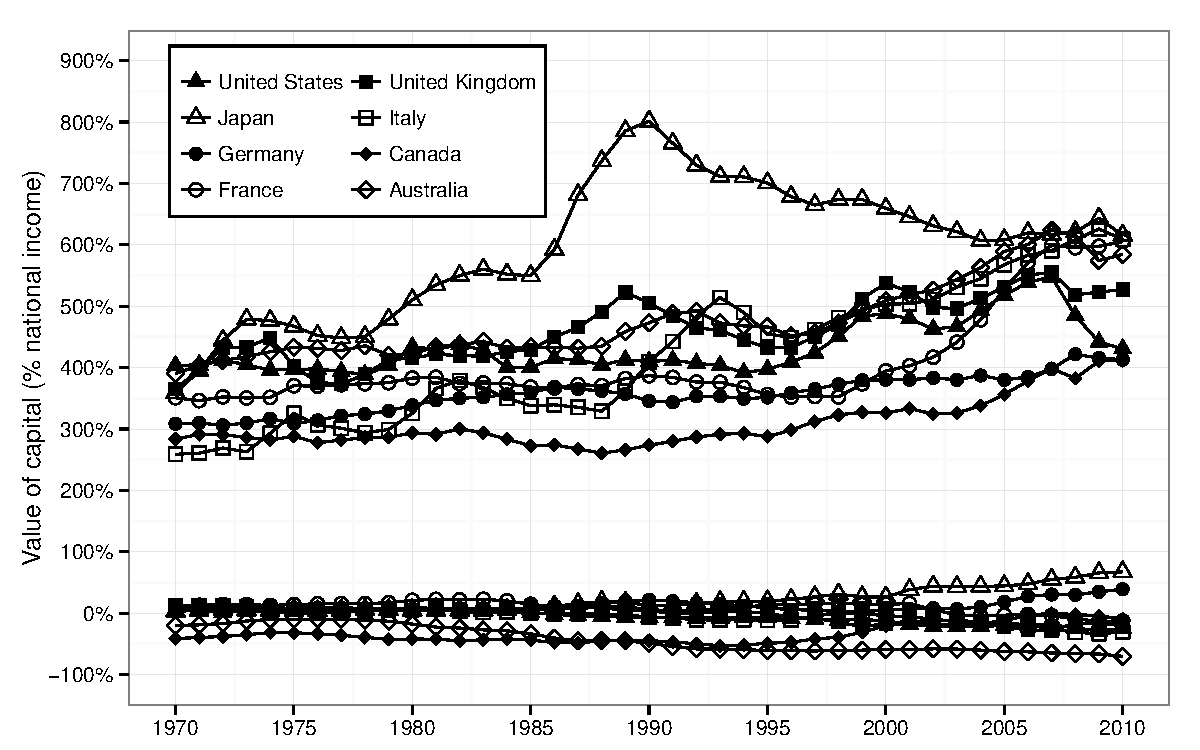
\includegraphics[width=1\linewidth]{figures/bw/Figure_5_7} 

}



\end{knitrout}
\caption{Net foreign assets held by Japan and Germany are worth between 6 months and one year of national income in 2010.}
\end{minipage}
\end{figure}
\end{frame}
%%%%%%%%%%%%%%%%%%%% Frame Here %%%%%%%%%%%%%%%%%%%%%%%%%%%%%%%%%%%%%%%%%%%%%%%%


%%%%%%%%%%%%%%%%%%%% Frame Here %%%%%%%%%%%%%%%%%%%%%%%%%%%%%%%%%%%%%%%%%%%%%%%%
\begin{frame}[label=Figure_5_7S]
\frametitle{Figure 5.7S. National capital in rich countries, 1970--2010}
\begin{figure}[t]
\begin{minipage}[b]{\textwidth}
\centering
\begin{knitrout}\footnotesize
\definecolor{shadecolor}{rgb}{0.969, 0.969, 0.969}\color{fgcolor}

{\centering \includegraphics[width=1\linewidth]{figures/bw/Figure_5_7S} 

}



\end{knitrout}
\caption{Net foreign assets held by Japan and Germany are worth between 6 months and one year of national income in 2010.}
\end{minipage}
\end{figure}
\end{frame}
%%%%%%%%%%%%%%%%%%%% Frame Here %%%%%%%%%%%%%%%%%%%%%%%%%%%%%%%%%%%%%%%%%%%%%%%%


%%%%%%%%%%%%%%%%%%%% Frame Here %%%%%%%%%%%%%%%%%%%%%%%%%%%%%%%%%%%%%%%%%%%%%%%%
\begin{frame}[label=Figure_5_8]
\frametitle{Figure 5.8. The world capital/income ratio, 1870--2100}
\begin{figure}[t]
\begin{minipage}[b]{\textwidth}
\centering
\begin{knitrout}\footnotesize
\definecolor{shadecolor}{rgb}{0.969, 0.969, 0.969}\color{fgcolor}

{\centering \includegraphics[width=1\linewidth]{figures/bw/Figure_5_8} 

}



\end{knitrout}
\caption{According to simulations (central scenario), the world capital/income ratio could be close to 700 percent by the end of the twenty-first century.}
\end{minipage}
\end{figure}
\end{frame}
%%%%%%%%%%%%%%%%%%%% Frame Here %%%%%%%%%%%%%%%%%%%%%%%%%%%%%%%%%%%%%%%%%%%%%%%%


%%%%%%%%%%%%%%%%%%%% Frame Here %%%%%%%%%%%%%%%%%%%%%%%%%%%%%%%%%%%%%%%%%%%%%%%%
\begin{frame}[label=Figure_S5_6]
\frametitle{Figure S5.6. Foreign assets and liabilities in the United States 1970--2010}
\begin{figure}[t]
\begin{minipage}[b]{\textwidth}
\centering
\begin{knitrout}\footnotesize
\definecolor{shadecolor}{rgb}{0.969, 0.969, 0.969}\color{fgcolor}

{\centering \includegraphics[width=\maxwidth]{figures/bw/Figure_S5_6} 

}



\end{knitrout}
\caption{Foreign liabilities (what the rest of the world owns in the US) have outweighted foreign assets (what the US own in the rest of the world) since 1985--1986.}
\end{minipage}
\end{figure}
\end{frame}
%%%%%%%%%%%%%%%%%%%% Frame Here %%%%%%%%%%%%%%%%%%%%%%%%%%%%%%%%%%%%%%%%%%%%%%%%


%%%%%%%%%%%%%%%%%%%% Frame Here %%%%%%%%%%%%%%%%%%%%%%%%%%%%%%%%%%%%%%%%%%%%%%%%
\begin{frame}[label=Figure_S5_7]
\frametitle{Figure S5.7. Foreign assets and liabilities in the Japan. 1970--2010}
\begin{figure}[t]
\begin{minipage}[b]{\textwidth}
\centering
\begin{knitrout}\footnotesize
\definecolor{shadecolor}{rgb}{0.969, 0.969, 0.969}\color{fgcolor}

{\centering \includegraphics[width=\maxwidth]{figures/bw/Figure_S5_7} 

}



\end{knitrout}
\caption{Foreign assets (what Japan owns in the rest of the world) are almost twice as large as foreign liabilities (what the rest of the world owns in Japan) in 2010.}
\end{minipage}
\end{figure}
\end{frame}
%%%%%%%%%%%%%%%%%%%% Frame Here %%%%%%%%%%%%%%%%%%%%%%%%%%%%%%%%%%%%%%%%%%%%%%%%


%%%%%%%%%%%%%%%%%%%% Frame Here %%%%%%%%%%%%%%%%%%%%%%%%%%%%%%%%%%%%%%%%%%%%%%%%
\begin{frame}[label=Figure_S5_8]
\frametitle{Figure S5.8. Foreign assets and liabilities in the Germany. 1970--2010}
\begin{figure}[t]
\begin{minipage}[b]{\textwidth}
\centering
\begin{knitrout}\footnotesize
\definecolor{shadecolor}{rgb}{0.969, 0.969, 0.969}\color{fgcolor}

{\centering \includegraphics[width=\maxwidth]{figures/bw/Figure_S5_8} 

}



\end{knitrout}
\caption{Foreign assets and liabilities in Germany have risen a lot since the 1980s--1990s.}
\end{minipage}
\end{figure}
\end{frame}
%%%%%%%%%%%%%%%%%%%% Frame Here %%%%%%%%%%%%%%%%%%%%%%%%%%%%%%%%%%%%%%%%%%%%%%%%


%%%%%%%%%%%%%%%%%%%% Frame Here %%%%%%%%%%%%%%%%%%%%%%%%%%%%%%%%%%%%%%%%%%%%%%%%
\begin{frame}[label=Figure_S5_9]
\frametitle{Figure S5.9. Foreign assets and liabilities in the France. 1970--2010}
\begin{figure}[t]
\begin{minipage}[b]{\textwidth}
\centering
\begin{knitrout}\footnotesize
\definecolor{shadecolor}{rgb}{0.969, 0.969, 0.969}\color{fgcolor}

{\centering \includegraphics[width=\maxwidth]{figures/bw/Figure_S5_9} 

}



\end{knitrout}
\caption{Like in Germany, foreign assets and liabilities have risen a lot since 1980s--1990s (but with a negative net position at the end of the period).}
\end{minipage}
\end{figure}
\end{frame}
%%%%%%%%%%%%%%%%%%%% Frame Here %%%%%%%%%%%%%%%%%%%%%%%%%%%%%%%%%%%%%%%%%%%%%%%%


%%%%%%%%%%%%%%%%%%%% Frame Here %%%%%%%%%%%%%%%%%%%%%%%%%%%%%%%%%%%%%%%%%%%%%%%%
\begin{frame}[label=Figure_S5_10]
\frametitle{Figure S5.10. Foreign assets and liabilities in the United Kingdom. 1970--2010}
\begin{figure}[t]
\begin{minipage}[b]{\textwidth}
\centering
\begin{knitrout}\footnotesize
\definecolor{shadecolor}{rgb}{0.969, 0.969, 0.969}\color{fgcolor}

{\centering \includegraphics[width=\maxwidth]{figures/bw/Figure_S5_10} 

}



\end{knitrout}
\caption{In the United Kingdom, foreign assets and liabilities reached 7--8 years of national income at the end of the period.}
\end{minipage}
\end{figure}
\end{frame}
%%%%%%%%%%%%%%%%%%%% Frame Here %%%%%%%%%%%%%%%%%%%%%%%%%%%%%%%%%%%%%%%%%%%%%%%%


%%%%%%%%%%%%%%%%%%%% Frame Here %%%%%%%%%%%%%%%%%%%%%%%%%%%%%%%%%%%%%%%%%%%%%%%%
\begin{frame}[label=Figure_S5_11]
\frametitle{Figure S5.11. Foreign assets and liabilities in the Spain. 1980--2010}
\begin{figure}[t]
\begin{minipage}[b]{\textwidth}
\centering
\begin{knitrout}\footnotesize
\definecolor{shadecolor}{rgb}{0.969, 0.969, 0.969}\color{fgcolor}

{\centering \includegraphics[width=\maxwidth]{figures/bw/Figure_S5_11} 

}



\end{knitrout}
\caption{Net foreign debt of Spain exceeds a year of national income in 2010.}
\end{minipage}
\end{figure}
\end{frame}
%%%%%%%%%%%%%%%%%%%% Frame Here %%%%%%%%%%%%%%%%%%%%%%%%%%%%%%%%%%%%%%%%%%%%%%%%


%%%%%%%%%%%%%%%%%%%% Frame Here %%%%%%%%%%%%%%%%%%%%%%%%%%%%%%%%%%%%%%%%%%%%%%%%
\begin{frame}[label=Figure_6_1]
\frametitle{Figure 6.1. The capital-labor split in Britain, 1770--2010}
\begin{figure}[t]
\begin{minipage}[b]{\textwidth}
\centering
\begin{knitrout}\footnotesize
\definecolor{shadecolor}{rgb}{0.969, 0.969, 0.969}\color{fgcolor}

{\centering \includegraphics[width=1\linewidth]{figures/bw/Figure_6_1} 

}



\end{knitrout}
\caption{During the nineteenth century, capital income (rent, profits, dividends, interest...) absorbed about 40 percent of national income versus 60 percent for labor income (including both wage and non-wage income).}
\end{minipage}
\end{figure}
\end{frame}
%%%%%%%%%%%%%%%%%%%% Frame Here %%%%%%%%%%%%%%%%%%%%%%%%%%%%%%%%%%%%%%%%%%%%%%%%


%%%%%%%%%%%%%%%%%%%% Frame Here %%%%%%%%%%%%%%%%%%%%%%%%%%%%%%%%%%%%%%%%%%%%%%%%
\begin{frame}[label=Figure_6_2]
\frametitle{Figure 6.2. The capital-labor split in France, 1820--2010}
\begin{figure}[t]
\begin{minipage}[b]{\textwidth}
\centering
\begin{knitrout}\footnotesize
\definecolor{shadecolor}{rgb}{0.969, 0.969, 0.969}\color{fgcolor}

{\centering \includegraphics[width=1\linewidth]{figures/bw/Figure_6_2} 

}



\end{knitrout}
\caption{In the twenty-first century, capital income (rent, profits, dividends, interest...) absorbs about 30 percent of national income versus 70 percent for labor income (including both wage and non-wage income).}
\end{minipage}
\end{figure}
\end{frame}
%%%%%%%%%%%%%%%%%%%% Frame Here %%%%%%%%%%%%%%%%%%%%%%%%%%%%%%%%%%%%%%%%%%%%%%%%


%%%%%%%%%%%%%%%%%%%% Frame Here %%%%%%%%%%%%%%%%%%%%%%%%%%%%%%%%%%%%%%%%%%%%%%%%
\begin{frame}[label=Figure_6_3]
\frametitle{Figure 6.3. The pure rate of return on capital in Britain, 1770--2010}
\begin{figure}[t]
\begin{minipage}[b]{\textwidth}
\centering
\begin{knitrout}\footnotesize
\definecolor{shadecolor}{rgb}{0.969, 0.969, 0.969}\color{fgcolor}

{\centering \includegraphics[width=1\linewidth]{figures/bw/Figure_6_3} 

}



\end{knitrout}
\caption{The pure rate of return to capital is roughly stable around 4--5 percent in the long run.}
\end{minipage}
\end{figure}
\end{frame}
%%%%%%%%%%%%%%%%%%%% Frame Here %%%%%%%%%%%%%%%%%%%%%%%%%%%%%%%%%%%%%%%%%%%%%%%%


%%%%%%%%%%%%%%%%%%%% Frame Here %%%%%%%%%%%%%%%%%%%%%%%%%%%%%%%%%%%%%%%%%%%%%%%%
\begin{frame}[label=Figure_6_4]
\frametitle{Figure 6.4. The pure rate of return on capital in France, 1820--2010}
\begin{figure}[t]
\begin{minipage}[b]{\textwidth}
\centering
\begin{knitrout}\footnotesize
\definecolor{shadecolor}{rgb}{0.969, 0.969, 0.969}\color{fgcolor}

{\centering \includegraphics[width=1\linewidth]{figures/bw/Figure_6_4} 

}



\end{knitrout}
\caption{The observed average rate of return displays larger fluctuations than the pure rate of return during the twentieth century.}
\end{minipage}
\end{figure}
\end{frame}
%%%%%%%%%%%%%%%%%%%% Frame Here %%%%%%%%%%%%%%%%%%%%%%%%%%%%%%%%%%%%%%%%%%%%%%%%


%%%%%%%%%%%%%%%%%%%% Frame Here %%%%%%%%%%%%%%%%%%%%%%%%%%%%%%%%%%%%%%%%%%%%%%%%
\begin{frame}[label=Figure_6_5]
\frametitle{Figure 6.5. The capital share in rich countries, 1975--2010}
\begin{figure}[t]
\begin{minipage}[b]{\textwidth}
\centering
\begin{knitrout}\footnotesize
\definecolor{shadecolor}{rgb}{0.969, 0.969, 0.969}\color{fgcolor}

{\centering \includegraphics[width=1\linewidth]{figures/bw/Figure_6_5} 

}



\end{knitrout}
\caption{Capital income absorbs between 15 percent and 25 percent of national income in rich countries in 1970, and between 25 percent and 30 percent in 2000--2010.}
\end{minipage}
\end{figure}
\end{frame}
%%%%%%%%%%%%%%%%%%%% Frame Here %%%%%%%%%%%%%%%%%%%%%%%%%%%%%%%%%%%%%%%%%%%%%%%%


%%%%%%%%%%%%%%%%%%%% Frame Here %%%%%%%%%%%%%%%%%%%%%%%%%%%%%%%%%%%%%%%%%%%%%%%%
\begin{frame}[label=Figure_6_6]
\frametitle{Figure 6.6. The profit share in the value added of corporations in France, 1900--2010}
\begin{figure}[t]
\begin{minipage}[b]{\textwidth}
\centering
\begin{knitrout}\footnotesize
\definecolor{shadecolor}{rgb}{0.969, 0.969, 0.969}\color{fgcolor}

{\centering \includegraphics[width=1\linewidth]{figures/bw/Figure_6_6} 

}



\end{knitrout}
\caption{The share of gross profits in gross value added of corporations rose from 25 percent in 1982 to 33 percent in 2010; the share of net profits in net value added rose from 12 percent to 20 percent.}
\end{minipage}
\end{figure}
\end{frame}
%%%%%%%%%%%%%%%%%%%% Frame Here %%%%%%%%%%%%%%%%%%%%%%%%%%%%%%%%%%%%%%%%%%%%%%%%


%%%%%%%%%%%%%%%%%%%% Frame Here %%%%%%%%%%%%%%%%%%%%%%%%%%%%%%%%%%%%%%%%%%%%%%%%
\begin{frame}[label=Figure_6_7]
\frametitle{Figure 6.7. The share of housing rent in national income in France, 1900--2010}
\begin{figure}[t]
\begin{minipage}[b]{\textwidth}
\centering
\begin{knitrout}\footnotesize
\definecolor{shadecolor}{rgb}{0.969, 0.969, 0.969}\color{fgcolor}

{\centering \includegraphics[width=1\linewidth]{figures/bw/Figure_6_7} 

}



\end{knitrout}
\caption{The share of housing rent (rental value of dwellings) rose from 2 percent of national income in 1948 to 10 percent in 2010.}
\end{minipage}
\end{figure}
\end{frame}
%%%%%%%%%%%%%%%%%%%% Frame Here %%%%%%%%%%%%%%%%%%%%%%%%%%%%%%%%%%%%%%%%%%%%%%%%


%%%%%%%%%%%%%%%%%%%% Frame Here %%%%%%%%%%%%%%%%%%%%%%%%%%%%%%%%%%%%%%%%%%%%%%%%
\begin{frame}[label=Figure_6_8]
\frametitle{Figure 6.8. The capital share in national income in France, 1900--2010}
\begin{figure}[t]
\begin{minipage}[b]{\textwidth}
\centering
\begin{knitrout}\footnotesize
\definecolor{shadecolor}{rgb}{0.969, 0.969, 0.969}\color{fgcolor}

{\centering \includegraphics[width=1\linewidth]{figures/bw/Figure_6_8} 

}



\end{knitrout}
\caption{The share of capital income (net profits and rents) rose from 15 percent of national income in 1982 to 27 percent in 2010.}
\end{minipage}
\end{figure}
\end{frame}
%%%%%%%%%%%%%%%%%%%% Frame Here %%%%%%%%%%%%%%%%%%%%%%%%%%%%%%%%%%%%%%%%%%%%%%%%


%%%%%%%%%%%%%%%%%%%% Frame Here %%%%%%%%%%%%%%%%%%%%%%%%%%%%%%%%%%%%%%%%%%%%%%%%
\begin{frame}[label=Figure_6_8S]
\frametitle{Figure 6.8S. The capital share in national income in France, 1900--2010}
\begin{figure}[t]
\begin{minipage}[b]{\textwidth}
\centering
\begin{knitrout}\footnotesize
\definecolor{shadecolor}{rgb}{0.969, 0.969, 0.969}\color{fgcolor}

{\centering \includegraphics[width=1\linewidth]{figures/bw/Figure_6_8S} 

}



\end{knitrout}
\caption{The share of capital income (net profits and rents) rose from 15 percent of national income in 1982 to 27 percent in 2010.}
\end{minipage}
\end{figure}
\end{frame}
%%%%%%%%%%%%%%%%%%%% Frame Here %%%%%%%%%%%%%%%%%%%%%%%%%%%%%%%%%%%%%%%%%%%%%%%%


%%%%%%%%%%%%%%%%%%%% Frame Here %%%%%%%%%%%%%%%%%%%%%%%%%%%%%%%%%%%%%%%%%%%%%%%%
\begin{frame}[label=Figure_7_1X]
\frametitle{Figure 7.1X. Examples of Gini-Lorenz curves}
\begin{figure}[t]
\begin{minipage}[b]{\textwidth}
\centering
\begin{knitrout}\footnotesize
\definecolor{shadecolor}{rgb}{0.969, 0.969, 0.969}\color{fgcolor}

{\centering \includegraphics[width=1\linewidth]{figures/bw/Figure_7_1X} 

}



\end{knitrout}
\caption{The share of capital income (net profits and rents) rose from 15 percent of national income in 1982 to 27 percent in 2010.}
\end{minipage}
\end{figure}
\end{frame}
%%%%%%%%%%%%%%%%%%%% Frame Here %%%%%%%%%%%%%%%%%%%%%%%%%%%%%%%%%%%%%%%%%%%%%%%%


%%%%%%%%%%%%%%%%%%%% Frame Here %%%%%%%%%%%%%%%%%%%%%%%%%%%%%%%%%%%%%%%%%%%%%%%%
\begin{frame}[label=Figure_8_1,fragile]
\frametitle{Figure 8.1. Income inequality in France, 1910--2010}
\begin{figure}[t]
\begin{minipage}[b]{\textwidth}
\centering
\begin{knitrout}\footnotesize
\definecolor{shadecolor}{rgb}{0.969, 0.969, 0.969}\color{fgcolor}

{\centering \includegraphics[width=1\linewidth]{figures/bw/Figure_8_1} 

}



\end{knitrout}
\caption{Inequality of total income (labor and capital) has dropped in France during the twentieth century, while wage inequality has remained the same.}
\end{minipage}
\end{figure}
\end{frame}
%%%%%%%%%%%%%%%%%%%% Frame Here %%%%%%%%%%%%%%%%%%%%%%%%%%%%%%%%%%%%%%%%%%%%%%%%


%%%%%%%%%%%%%%%%%%%% Frame Here %%%%%%%%%%%%%%%%%%%%%%%%%%%%%%%%%%%%%%%%%%%%%%%%
\begin{frame}[label=Figure_8_2,fragile]
\frametitle{Figure 8.2. The fall of rentiers in France, 1910--2010}
\begin{figure}[t]
\begin{minipage}[b]{\textwidth}
\centering
\begin{knitrout}\footnotesize
\definecolor{shadecolor}{rgb}{0.969, 0.969, 0.969}\color{fgcolor}

{\centering \includegraphics[width=1\linewidth]{figures/bw/Figure_8_2} 

}



\end{knitrout}
\caption{The fall in the top percentile share (the top 1 percent highest incomes) in France between 1914 and 1945 is due to the fall of top capital incomes.}
\end{minipage}
\end{figure}
\end{frame}
%%%%%%%%%%%%%%%%%%%% Frame Here %%%%%%%%%%%%%%%%%%%%%%%%%%%%%%%%%%%%%%%%%%%%%%%%


%%%%%%%%%%%%%%%%%%%% Frame Here %%%%%%%%%%%%%%%%%%%%%%%%%%%%%%%%%%%%%%%%%%%%%%%%
\begin{frame}[label=Figure_8_3,fragile]
\frametitle{Figure 8.3. The composition of top incomes in France in 1932}
\begin{figure}[t]
\begin{minipage}[b]{\textwidth}
\centering
\begin{knitrout}\footnotesize
\definecolor{shadecolor}{rgb}{0.969, 0.969, 0.969}\color{fgcolor}

{\centering \includegraphics[width=1\linewidth]{figures/bw/Figure_8_3} 

}



\end{knitrout}
\caption{\scriptsize{Labor income becomes less and less important as one goes up within the top decile of total income. Notes: (i)~``P90--95'' includes individuals between percentiles 90 to 95, ``P95--99'' includes the next 4 percent, ``P99--99.5'' the next 0.5 percent, etc.; (ii)~Labor income: wages, bonuses, pensions. Capital income: dividends, interest, rent. Mixed income: self-employment income.}}
\end{minipage}
\end{figure}
\end{frame}
%%%%%%%%%%%%%%%%%%%% Frame Here %%%%%%%%%%%%%%%%%%%%%%%%%%%%%%%%%%%%%%%%%%%%%%%%


%%%%%%%%%%%%%%%%%%%% Frame Here %%%%%%%%%%%%%%%%%%%%%%%%%%%%%%%%%%%%%%%%%%%%%%%%
\begin{frame}[label=Figure_8_4,fragile]
\frametitle{Figure 8.4. The composition of top incomes in France in 2005}
\begin{figure}[t]
\begin{minipage}[b]{\textwidth}
\centering
\begin{knitrout}\footnotesize
\definecolor{shadecolor}{rgb}{0.969, 0.969, 0.969}\color{fgcolor}

{\centering \includegraphics[width=1\linewidth]{figures/bw/Figure_8_4} 

}



\end{knitrout}
\caption{Capital income becomes dominant at the level of the top 0.1 percent in France in 2005, as opposed to the top 0.5 percent in 1932.}
\end{minipage}
\end{figure}
\end{frame}
%%%%%%%%%%%%%%%%%%%% Frame Here %%%%%%%%%%%%%%%%%%%%%%%%%%%%%%%%%%%%%%%%%%%%%%%%


%%%%%%%%%%%%%%%%%%%% Frame Here %%%%%%%%%%%%%%%%%%%%%%%%%%%%%%%%%%%%%%%%%%%%%%%%
\begin{frame}[label=Figure_8_5,fragile]
\frametitle{Figure 8.5. Income inequality in the United States, 1910--2010}
\begin{figure}[t]
\begin{minipage}[b]{\textwidth}
\centering
\begin{knitrout}\footnotesize
\definecolor{shadecolor}{rgb}{0.969, 0.969, 0.969}\color{fgcolor}

{\centering \includegraphics[width=1\linewidth]{figures/bw/Figure_8_5} 

}



\end{knitrout}
\caption{The top decile share in U.S. national income dropped from 45--50\% in the 1910s--1920s to less than 35\% in the 1950s (this is the
1950 1960 fall documented by Kuznets); it then rose from less than 35\% in the 1970s to 45--50\% in the 2000s--2010s.}
\end{minipage}
\end{figure}
\end{frame}
%%%%%%%%%%%%%%%%%%%% Frame Here %%%%%%%%%%%%%%%%%%%%%%%%%%%%%%%%%%%%%%%%%%%%%%%%


%%%%%%%%%%%%%%%%%%%% Frame Here %%%%%%%%%%%%%%%%%%%%%%%%%%%%%%%%%%%%%%%%%%%%%%%%
\begin{frame}[label=Figure_8_6,fragile]
\frametitle{Figure 8.6. Decomposition of the top decile, United States, 1910--2010}
\begin{figure}[t]
\begin{minipage}[b]{\textwidth}
\centering
\begin{knitrout}\footnotesize
\definecolor{shadecolor}{rgb}{0.969, 0.969, 0.969}\color{fgcolor}

{\centering \includegraphics[width=1\linewidth]{figures/bw/Figure_8_6} 

}



\end{knitrout}
\caption{The rise of the top decile income share since the 1970s is mostly due to the top percentile.}
\end{minipage}
\end{figure}
\end{frame}
%%%%%%%%%%%%%%%%%%%% Frame Here %%%%%%%%%%%%%%%%%%%%%%%%%%%%%%%%%%%%%%%%%%%%%%%%


%%%%%%%%%%%%%%%%%%%% Frame Here %%%%%%%%%%%%%%%%%%%%%%%%%%%%%%%%%%%%%%%%%%%%%%%%
\begin{frame}[label=Figure_8_7,fragile]
\frametitle{Figure 8.7. High incomes and high wages in the United States, 1910--2010}
\begin{figure}[t]
\begin{minipage}[b]{\textwidth}
\centering
\begin{knitrout}\footnotesize
\definecolor{shadecolor}{rgb}{0.969, 0.969, 0.969}\color{fgcolor}

{\centering \includegraphics[width=1\linewidth]{figures/bw/Figure_8_7} 

}



\end{knitrout}
\caption{The rise of income inequality since the 1970s is largely due to the rise of wage inequality.}
\end{minipage}
\end{figure}
\end{frame}
%%%%%%%%%%%%%%%%%%%% Frame Here %%%%%%%%%%%%%%%%%%%%%%%%%%%%%%%%%%%%%%%%%%%%%%%%


%%%%%%%%%%%%%%%%%%%% Frame Here %%%%%%%%%%%%%%%%%%%%%%%%%%%%%%%%%%%%%%%%%%%%%%%%
\begin{frame}[label=Figure_8_8,fragile]
\frametitle{Figure 8.8. The transformation of the top 1 percent in the United States, 1910--2010}
\begin{figure}[t]
\begin{minipage}[b]{\textwidth}
\centering 
\begin{knitrout}\footnotesize
\definecolor{shadecolor}{rgb}{0.969, 0.969, 0.969}\color{fgcolor}

{\centering \includegraphics[width=1\linewidth]{figures/bw/Figure_8_8} 

}



\end{knitrout}
\caption{The rise in the top 1 percent highest incomes since the 1970s is largely due to the rise in the top 1 percent highest wages.}
\end{minipage}
\end{figure}
\end{frame}
%%%%%%%%%%%%%%%%%%%% Frame Here %%%%%%%%%%%%%%%%%%%%%%%%%%%%%%%%%%%%%%%%%%%%%%%%


%%%%%%%%%%%%%%%%%%%% Frame Here %%%%%%%%%%%%%%%%%%%%%%%%%%%%%%%%%%%%%%%%%%%%%%%%
\begin{frame}[label=Figure_8_9,fragile]
\frametitle{Figure 8.9. The composition of top incomes in the United States in 1929}
\begin{figure}[t]
\begin{minipage}[b]{\textwidth}
\centering
\begin{knitrout}\footnotesize
\definecolor{shadecolor}{rgb}{0.969, 0.969, 0.969}\color{fgcolor}

{\centering \includegraphics[width=1\linewidth]{figures/bw/Figure_8_9} 

}



\end{knitrout}
\caption{Labor income becomes less and less important as one moves up within the top income decile.}
\end{minipage}
\end{figure}
\end{frame}
%%%%%%%%%%%%%%%%%%%% Frame Here %%%%%%%%%%%%%%%%%%%%%%%%%%%%%%%%%%%%%%%%%%%%%%%%


%%%%%%%%%%%%%%%%%%%% Frame Here %%%%%%%%%%%%%%%%%%%%%%%%%%%%%%%%%%%%%%%%%%%%%%%%
\begin{frame}[label=Figure_8_10,fragile]
\frametitle{Figure 8.10. The composition of top incomes in the United States in 2007}
\begin{figure}[t]
\begin{minipage}[b]{\textwidth}
\centering
\begin{knitrout}\footnotesize
\definecolor{shadecolor}{rgb}{0.969, 0.969, 0.969}\color{fgcolor}

{\centering \includegraphics[width=1\linewidth]{figures/bw/Figure_8_10} 

}



\end{knitrout}
\caption{Capital income becomes dominant at the level of top 0.1 percent in 2007, as opposed to the top 1 percent in 1929.}
\end{minipage}
\end{figure}
\end{frame}
%%%%%%%%%%%%%%%%%%%% Frame Here %%%%%%%%%%%%%%%%%%%%%%%%%%%%%%%%%%%%%%%%%%%%%%%%


%%%%%%%%%%%%%%%%%%%% Frame Here %%%%%%%%%%%%%%%%%%%%%%%%%%%%%%%%%%%%%%%%%%%%%%%%
\begin{frame}[label=Figure_9_1]
\frametitle{Figure 9.1. Minimum wage in France and the United States, 1950--2013}
\begin{figure}[t]
\begin{minipage}[b]{\textwidth}
\centering

\begin{knitrout}\footnotesize
\definecolor{shadecolor}{rgb}{0.969, 0.969, 0.969}\color{fgcolor}

{\centering \includegraphics[width=1\linewidth]{figures/bw/Figure_9_1} 

}



\end{knitrout}
\caption{Expressed in 2013 purchasing power, the hourly minimum wage rose from \$3.80 to \$7.30 between 1950 and 2013 in the United States, and from \euro 2.10 to \euro 9.40 in France.}
\end{minipage}
\end{figure}
\end{frame}
%%%%%%%%%%%%%%%%%%%% Frame Here %%%%%%%%%%%%%%%%%%%%%%%%%%%%%%%%%%%%%%%%%%%%%%%%


%%%%%%%%%%%%%%%%%%%% Frame Here %%%%%%%%%%%%%%%%%%%%%%%%%%%%%%%%%%%%%%%%%%%%%%%%
\begin{frame}[label=Figure_S9_1]
\frametitle{Figure S9.1. Minimum wage in France, 1950--2013}
\begin{figure}[t]
\begin{minipage}[b]{\textwidth}
\centering
\begin{knitrout}\footnotesize
\definecolor{shadecolor}{rgb}{0.969, 0.969, 0.969}\color{fgcolor}

{\centering \includegraphics[width=\maxwidth]{figures/bw/Figure_S9_1} 

}



\end{knitrout}
\caption{Expressed in 2013 purchasing power, the hourly minimum wage rose from \euro 2.10 to \euro 9.40 in France between 1950 and 2013.}
\end{minipage}
\end{figure}
\end{frame}
%%%%%%%%%%%%%%%%%%%% Frame Here %%%%%%%%%%%%%%%%%%%%%%%%%%%%%%%%%%%%%%%%%%%%%%%%


%%%%%%%%%%%%%%%%%%%% Frame Here %%%%%%%%%%%%%%%%%%%%%%%%%%%%%%%%%%%%%%%%%%%%%%%%
\begin{frame}[label=Figure_S9_2]
\frametitle{Figure S9.2. Minimum wage in United States, 1950--2013}
\begin{figure}[t]
\begin{minipage}[b]{\textwidth}
\centering
\begin{knitrout}\footnotesize
\definecolor{shadecolor}{rgb}{0.969, 0.969, 0.969}\color{fgcolor}

{\centering \includegraphics[width=\maxwidth]{figures/bw/Figure_S9_2} 

}



\end{knitrout}
\caption{Expressed in 2013 purchasing power, the hourly minimum wage rose from \$3.80 to \$7.30 in the United States between 1950 and 2013.}
\end{minipage}
\end{figure}
\end{frame}
%%%%%%%%%%%%%%%%%%%% Frame Here %%%%%%%%%%%%%%%%%%%%%%%%%%%%%%%%%%%%%%%%%%%%%%%%


%%%%%%%%%%%%%%%%%%%% Frame Here %%%%%%%%%%%%%%%%%%%%%%%%%%%%%%%%%%%%%%%%%%%%%%%%
\begin{frame}[label=Figure_9_2]
\frametitle{Figure 9.2. Income inequality in Anglo-Saxon countries, 1910--2010}
\begin{figure}[t]
\begin{minipage}[b]{\textwidth}
\centering
\begin{knitrout}\footnotesize
\definecolor{shadecolor}{rgb}{0.969, 0.969, 0.969}\color{fgcolor}

{\centering \includegraphics[width=1\linewidth]{figures/bw/Figure_9_2} 

}



\end{knitrout}
\caption{The share of top percentile in total income rose since the 1970s in all Anglo-Saxon countries, but with different magnitudes.}
\end{minipage}
\end{figure}
\end{frame}
%%%%%%%%%%%%%%%%%%%% Frame Here %%%%%%%%%%%%%%%%%%%%%%%%%%%%%%%%%%%%%%%%%%%%%%%%


%%%%%%%%%%%%%%%%%%%% Frame Here %%%%%%%%%%%%%%%%%%%%%%%%%%%%%%%%%%%%%%%%%%%%%%%%
\begin{frame}[label=Figure_9_3]
\frametitle{Figure 9.3. Income inequality in Continental Europe and Japan, 1910--2010}
\begin{figure}[t]
\begin{minipage}[b]{\textwidth}
\centering
\begin{knitrout}\footnotesize
\definecolor{shadecolor}{rgb}{0.969, 0.969, 0.969}\color{fgcolor}

{\centering \includegraphics[width=1\linewidth]{figures/bw/Figure_9_3} 

}



\end{knitrout}
\caption{As compared to Anglo-Saxon countries, the share of top percentile barely increased since the 1970s in Continental Europe and Japan.}
\end{minipage}
\end{figure}
\end{frame}
%%%%%%%%%%%%%%%%%%%% Frame Here %%%%%%%%%%%%%%%%%%%%%%%%%%%%%%%%%%%%%%%%%%%%%%%%


%%%%%%%%%%%%%%%%%%%% Frame Here %%%%%%%%%%%%%%%%%%%%%%%%%%%%%%%%%%%%%%%%%%%%%%%%
\begin{frame}[label=Figure_9_4]
\frametitle{Figure 9.4. Income inequality in Northern and Southern Europe, 1910--2010}
\begin{figure}[t]
\begin{minipage}[b]{\textwidth}
\centering
\begin{knitrout}\footnotesize
\definecolor{shadecolor}{rgb}{0.969, 0.969, 0.969}\color{fgcolor}

{\centering \includegraphics[width=1\linewidth]{figures/bw/Figure_9_4} 

}



\end{knitrout}
\caption{As compared to Anglo-Saxon countries, the top percentile income share barely increased in Northern and Southern Europe since the 1970s.}
\end{minipage}
\end{figure}
\end{frame}
%%%%%%%%%%%%%%%%%%%% Frame Here %%%%%%%%%%%%%%%%%%%%%%%%%%%%%%%%%%%%%%%%%%%%%%%%


%%%%%%%%%%%%%%%%%%%% Frame Here %%%%%%%%%%%%%%%%%%%%%%%%%%%%%%%%%%%%%%%%%%%%%%%%
\begin{frame}[label=Figure_9_5]
\frametitle{Figure 9.5. The top 0.1\% income share in Anglo-Saxon countries, 1910--2010}
\begin{figure}[t]
\begin{minipage}[b]{\textwidth}
\centering
\begin{knitrout}\footnotesize
\definecolor{shadecolor}{rgb}{0.969, 0.969, 0.969}\color{fgcolor}

{\centering \includegraphics[width=1\linewidth]{figures/bw/Figure_9_5} 

}



\end{knitrout}
\caption{The share of the top 0.1 percent highest incomes in total income rose sharply since the 1970s in all Anglo-Saxon countries, but with varying magnitudes.}
\end{minipage}
\end{figure}
\end{frame}
%%%%%%%%%%%%%%%%%%%% Frame Here %%%%%%%%%%%%%%%%%%%%%%%%%%%%%%%%%%%%%%%%%%%%%%%%


%%%%%%%%%%%%%%%%%%%% Frame Here %%%%%%%%%%%%%%%%%%%%%%%%%%%%%%%%%%%%%%%%%%%%%%%%
\begin{frame}[label=Figure_9_5X]
\frametitle{Figure 9.5X. The top decile income share in Anglo-Saxon countries, 1910--2010}
\begin{figure}[t]
\begin{minipage}[b]{\textwidth}
\centering
\begin{knitrout}\footnotesize
\definecolor{shadecolor}{rgb}{0.969, 0.969, 0.969}\color{fgcolor}

{\centering \includegraphics[width=1\linewidth]{figures/bw/Figure_9_5X} 

}



\end{knitrout}
\caption{The share of the top decile of highest incomes rose sharply in the 1980s and 1990s in all Anglo-Saxon countries, and in particular in the United States and United Kingdom.}
\end{minipage}
\end{figure}
\end{frame}
%%%%%%%%%%%%%%%%%%%% Frame Here %%%%%%%%%%%%%%%%%%%%%%%%%%%%%%%%%%%%%%%%%%%%%%%%


%%%%%%%%%%%%%%%%%%%% Frame Here %%%%%%%%%%%%%%%%%%%%%%%%%%%%%%%%%%%%%%%%%%%%%%%%
\begin{frame}[label=Figure_9_6]
\frametitle{Figure 9.6. The top 0.1\% income share in Continental Europe and Japan, 1910--2010}
\begin{figure}[t]
\begin{minipage}[b]{\textwidth}
\centering
\begin{knitrout}\footnotesize
\definecolor{shadecolor}{rgb}{0.969, 0.969, 0.969}\color{fgcolor}

{\centering \includegraphics[width=1\linewidth]{figures/bw/Figure_9_6} 

}



\end{knitrout}
\caption{As compared to Anglo-Saxon countries, the top 0.1 percent income share barely increased in Continental Europe and Japan.}
\end{minipage}
\end{figure}
\end{frame}
%%%%%%%%%%%%%%%%%%%% Frame Here %%%%%%%%%%%%%%%%%%%%%%%%%%%%%%%%%%%%%%%%%%%%%%%%


%%%%%%%%%%%%%%%%%%%% Frame Here %%%%%%%%%%%%%%%%%%%%%%%%%%%%%%%%%%%%%%%%%%%%%%%%
\begin{frame}[label=Figure_9_6X]
\frametitle{Figure 9.6X. The top decile income share in Continental Europe and Japan, 1910--2010}
\begin{figure}[t]
\begin{minipage}[b]{\textwidth}
\centering
\begin{knitrout}\footnotesize
\definecolor{shadecolor}{rgb}{0.969, 0.969, 0.969}\color{fgcolor}

{\centering \includegraphics[width=1\linewidth]{figures/bw/Figure_9_6X} 

}



\end{knitrout}
\caption{As compared to Anglo-Saxon countries, the top 10 percent income share has barely increased in Continental Europe.}
\end{minipage}
\end{figure}
\end{frame}
%%%%%%%%%%%%%%%%%%%% Frame Here %%%%%%%%%%%%%%%%%%%%%%%%%%%%%%%%%%%%%%%%%%%%%%%%


%%%%%%%%%%%%%%%%%%%% Frame Here %%%%%%%%%%%%%%%%%%%%%%%%%%%%%%%%%%%%%%%%%%%%%%%%
\begin{frame}[label=Figure_9_7]
\frametitle{Figure 9.7. The top decile income share in Europe and the United States, 1900--2010}
\begin{figure}[t]
\begin{minipage}[b]{\textwidth}
\centering
\begin{knitrout}\footnotesize
\definecolor{shadecolor}{rgb}{0.969, 0.969, 0.969}\color{fgcolor}

{\centering \includegraphics[width=1\linewidth]{figures/bw/Figure_9_7} 

}



\end{knitrout}
\caption{In the 1950s--1970s, the top decile income share was about 30--35 percent of total income in Europe as in the United States.}
\end{minipage}
\end{figure}
\end{frame}
%%%%%%%%%%%%%%%%%%%% Frame Here %%%%%%%%%%%%%%%%%%%%%%%%%%%%%%%%%%%%%%%%%%%%%%%%


%%%%%%%%%%%%%%%%%%%% Frame Here %%%%%%%%%%%%%%%%%%%%%%%%%%%%%%%%%%%%%%%%%%%%%%%%
\begin{frame}[label=Figure_9_7X]
\frametitle{Figure 9.7X. The top 0.1\% income share in Europe and the United States, 1900--2010}
\begin{figure}[t]
\begin{minipage}[b]{\textwidth}
\centering
\begin{knitrout}\footnotesize
\definecolor{shadecolor}{rgb}{0.969, 0.969, 0.969}\color{fgcolor}

{\centering \includegraphics[width=1\linewidth]{figures/bw/Figure_9_7X} 

}



\end{knitrout}
\caption{In the 1950s the top 0.1\% income share was about 2--4\% percent of total income in Europe and in the United States.}
\end{minipage}
\end{figure}
\end{frame}
%%%%%%%%%%%%%%%%%%%% Frame Here %%%%%%%%%%%%%%%%%%%%%%%%%%%%%%%%%%%%%%%%%%%%%%%%


%%%%%%%%%%%%%%%%%%%% Frame Here %%%%%%%%%%%%%%%%%%%%%%%%%%%%%%%%%%%%%%%%%%%%%%%%
\begin{frame}[label=Figure_9_8]
\frametitle{Figure 9.8: Income inequality: Europe vs. United States, 1900--2010}
\begin{figure}[t]
\begin{minipage}[b]{\textwidth}
\centering
\begin{knitrout}\footnotesize
\definecolor{shadecolor}{rgb}{0.969, 0.969, 0.969}\color{fgcolor}

{\centering \includegraphics[width=1\linewidth]{figures/bw/Figure_9_8} 

}



\end{knitrout}
\caption{The top decile income share was higher in Europe than in the U.S. in 1900--2010. It is much higher in the U.S. in 2000--2010.}
\end{minipage}
\end{figure}
\end{frame}
%%%%%%%%%%%%%%%%%%%% Frame Here %%%%%%%%%%%%%%%%%%%%%%%%%%%%%%%%%%%%%%%%%%%%%%%%


%%%%%%%%%%%%%%%%%%%% Frame Here %%%%%%%%%%%%%%%%%%%%%%%%%%%%%%%%%%%%%%%%%%%%%%%%
\begin{frame}[label=Figure_9_9]
\frametitle{Figure 9.9. Income inequality in emerging countries, 1910--2010}
\begin{figure}[t]
\begin{minipage}[b]{\textwidth}
\centering
\begin{knitrout}\footnotesize
\definecolor{shadecolor}{rgb}{0.969, 0.969, 0.969}\color{fgcolor}

{\centering \includegraphics[width=1\linewidth]{figures/bw/Figure_9_9} 

}



\end{knitrout}
\caption{Measured by the top percentile income share, income inequality rose in emerging countries since the 1980s, but ranks below the US level in 2000--2010.}
\end{minipage}
\end{figure}
\end{frame}
%%%%%%%%%%%%%%%%%%%% Frame Here %%%%%%%%%%%%%%%%%%%%%%%%%%%%%%%%%%%%%%%%%%%%%%%%


%%%%%%%%%%%%%%%%%%%% Frame Here %%%%%%%%%%%%%%%%%%%%%%%%%%%%%%%%%%%%%%%%%%%%%%%%
\begin{frame}[label=Figure_10_1]
\frametitle{Figure 10.1. Wealth inequality in France, 1810--2010}
\begin{figure}[t]
\begin{minipage}[b]{\textwidth}
\centering
\begin{knitrout}\footnotesize
\definecolor{shadecolor}{rgb}{0.969, 0.969, 0.969}\color{fgcolor}

{\centering \includegraphics[width=1\linewidth]{figures/bw/Figure_10_1} 

}



\end{knitrout}
\caption{The top decile (the top 10 percent highest wealth holders) owns 80--90 percent of total wealth in 1810--1910, and 60--65 percent today.}
\end{minipage}
\end{figure}
\end{frame}
%%%%%%%%%%%%%%%%%%%% Frame Here %%%%%%%%%%%%%%%%%%%%%%%%%%%%%%%%%%%%%%%%%%%%%%%%


%%%%%%%%%%%%%%%%%%%% Frame Here %%%%%%%%%%%%%%%%%%%%%%%%%%%%%%%%%%%%%%%%%%%%%%%%
\begin{frame}[label=Figure_10_1S]
\frametitle{Figure 10.1S. Wealth inequality in France, 1810--2010}
\begin{figure}[t]
\begin{minipage}[b]{\textwidth}
\centering
\begin{knitrout}\footnotesize
\definecolor{shadecolor}{rgb}{0.969, 0.969, 0.969}\color{fgcolor}

{\centering \includegraphics[width=1\linewidth]{figures/bw/Figure_10_1S} 

}



\end{knitrout}
\caption{The top decile (the top 10 percent highest wealth holders) owns 80--90 percent of total wealth in 1810--1910, and 60--65 percent today.}
\end{minipage}
\end{figure}
\end{frame}
%%%%%%%%%%%%%%%%%%%% Frame Here %%%%%%%%%%%%%%%%%%%%%%%%%%%%%%%%%%%%%%%%%%%%%%%%


%%%%%%%%%%%%%%%%%%%% Frame Here %%%%%%%%%%%%%%%%%%%%%%%%%%%%%%%%%%%%%%%%%%%%%%%%
\begin{frame}[label=Figure_10_2]
\frametitle{Figure 10.2. Wealth inequality in Paris versus France, 1810--2010}
\begin{figure}[t]
\begin{minipage}[b]{\textwidth}
\centering
\begin{knitrout}\footnotesize
\definecolor{shadecolor}{rgb}{0.969, 0.969, 0.969}\color{fgcolor}

{\centering \includegraphics[width=1\linewidth]{figures/bw/Figure_10_2} 

}



\end{knitrout}
\caption{The top percentile (the top 1 percent wealth holders) owns 70 percent of aggregate wealth in Paris on the eve of World War I.}
\end{minipage}
\end{figure}
\end{frame}
%%%%%%%%%%%%%%%%%%%% Frame Here %%%%%%%%%%%%%%%%%%%%%%%%%%%%%%%%%%%%%%%%%%%%%%%%


%%%%%%%%%%%%%%%%%%%% Frame Here %%%%%%%%%%%%%%%%%%%%%%%%%%%%%%%%%%%%%%%%%%%%%%%%
\begin{frame}[label=Figure_10_3]
\frametitle{Figure 10.3. Wealth inequality in Britain, 1810--2010}
\begin{figure}[t]
\begin{minipage}[b]{\textwidth}
\centering
\begin{knitrout}\footnotesize
\definecolor{shadecolor}{rgb}{0.969, 0.969, 0.969}\color{fgcolor}

{\centering \includegraphics[width=1\linewidth]{figures/bw/Figure_10_3} 

}



\end{knitrout}
\caption{The top decile owns 80--90 percent of total wealth in 1810--1910, and 70 percent today.}
\end{minipage}
\end{figure}
\end{frame}
%%%%%%%%%%%%%%%%%%%% Frame Here %%%%%%%%%%%%%%%%%%%%%%%%%%%%%%%%%%%%%%%%%%%%%%%%


%%%%%%%%%%%%%%%%%%%% Frame Here %%%%%%%%%%%%%%%%%%%%%%%%%%%%%%%%%%%%%%%%%%%%%%%%
\begin{frame}[label=Figure_10_3S]
\frametitle{Figure 10.3S. Wealth inequality in the United Kingdom, 1810--2010}
\begin{figure}[t]
\begin{minipage}[b]{\textwidth}
\centering
\begin{knitrout}\footnotesize
\definecolor{shadecolor}{rgb}{0.969, 0.969, 0.969}\color{fgcolor}

{\centering \includegraphics[width=1\linewidth]{figures/bw/Figure_10_3S} 

}



\end{knitrout}
\caption{The top decile owns 80--90 percent of total wealth in 1810--1910, and 70 percent today.}
\end{minipage}
\end{figure}
\end{frame}
%%%%%%%%%%%%%%%%%%%% Frame Here %%%%%%%%%%%%%%%%%%%%%%%%%%%%%%%%%%%%%%%%%%%%%%%%


%%%%%%%%%%%%%%%%%%%% Frame Here %%%%%%%%%%%%%%%%%%%%%%%%%%%%%%%%%%%%%%%%%%%%%%%%
\begin{frame}[label=Figure_10_4]
\frametitle{Figure 10.4. Wealth inequality in Sweden, 1810--2010}
\begin{figure}[t]
\begin{minipage}[b]{\textwidth}
\centering
\begin{knitrout}\footnotesize
\definecolor{shadecolor}{rgb}{0.969, 0.969, 0.969}\color{fgcolor}

{\centering \includegraphics[width=1\linewidth]{figures/bw/Figure_10_4} 

}



\end{knitrout}
\caption{The top 10 percent holds 80--90 percent of total wealth in 1810--1910 and 55--60 percent today.}
\end{minipage}
\end{figure}
\end{frame}
%%%%%%%%%%%%%%%%%%%% Frame Here %%%%%%%%%%%%%%%%%%%%%%%%%%%%%%%%%%%%%%%%%%%%%%%%


%%%%%%%%%%%%%%%%%%%% Frame Here %%%%%%%%%%%%%%%%%%%%%%%%%%%%%%%%%%%%%%%%%%%%%%%%
\begin{frame}[label=Figure_10_4S]
\frametitle{Figure 10.4S. Wealth inequality in Sweden, 1810--2010}
\begin{figure}[t]
\begin{minipage}[b]{\textwidth}
\centering
\begin{knitrout}\footnotesize
\definecolor{shadecolor}{rgb}{0.969, 0.969, 0.969}\color{fgcolor}

{\centering \includegraphics[width=1\linewidth]{figures/bw/Figure_10_4S} 

}



\end{knitrout}
\caption{The top 10 percent holds 80--90 percent of total wealth in 1810--1910 and 55--60 percent today.}
\end{minipage}
\end{figure}
\end{frame}
%%%%%%%%%%%%%%%%%%%% Frame Here %%%%%%%%%%%%%%%%%%%%%%%%%%%%%%%%%%%%%%%%%%%%%%%%


%%%%%%%%%%%%%%%%%%%% Frame Here %%%%%%%%%%%%%%%%%%%%%%%%%%%%%%%%%%%%%%%%%%%%%%%%
\begin{frame}[label=Figure_10_5]
\frametitle{Figure 10.5. Wealth inequality in the United States, 1810--2010}
\begin{figure}[t]
\begin{minipage}[b]{\textwidth}
\centering
\begin{knitrout}\footnotesize
\definecolor{shadecolor}{rgb}{0.969, 0.969, 0.969}\color{fgcolor}

{\centering \includegraphics[width=1\linewidth]{figures/bw/Figure_10_5} 

}



\end{knitrout}
\caption{The top 10 percent wealth holders own about 80 percent of total wealth in 1910 and 75 percent today.}
\end{minipage}
\end{figure}
\end{frame}
%%%%%%%%%%%%%%%%%%%% Frame Here %%%%%%%%%%%%%%%%%%%%%%%%%%%%%%%%%%%%%%%%%%%%%%%%


%%%%%%%%%%%%%%%%%%%% Frame Here %%%%%%%%%%%%%%%%%%%%%%%%%%%%%%%%%%%%%%%%%%%%%%%%
\begin{frame}[label=Figure_10_5S]
\frametitle{Figure 10.5S. Wealth inequality in the United States, 1810--2010}
\begin{figure}[t]
\begin{minipage}[b]{\textwidth}
\centering
\begin{knitrout}\footnotesize
\definecolor{shadecolor}{rgb}{0.969, 0.969, 0.969}\color{fgcolor}

{\centering \includegraphics[width=1\linewidth]{figures/bw/Figure_10_5S} 

}



\end{knitrout}
\caption{The top 10 percent wealth holders own about 80 percent of total wealth in 1910 and 75 percent today.}
\end{minipage}
\end{figure}
\end{frame}
%%%%%%%%%%%%%%%%%%%% Frame Here %%%%%%%%%%%%%%%%%%%%%%%%%%%%%%%%%%%%%%%%%%%%%%%%


%%%%%%%%%%%%%%%%%%%% Frame Here %%%%%%%%%%%%%%%%%%%%%%%%%%%%%%%%%%%%%%%%%%%%%%%%
\begin{frame}[label=Figure_10_6]
\frametitle{Figure 10.6. Wealth inequality in Europe versus the United States, 1810--2010}
\begin{figure}[t]
\begin{minipage}[b]{\textwidth}
\centering
\begin{knitrout}\footnotesize
\definecolor{shadecolor}{rgb}{0.969, 0.969, 0.969}\color{fgcolor}

{\centering \includegraphics[width=1\linewidth]{figures/bw/Figure_10_6} 

}



\end{knitrout}
\caption{Until the mid-twentieth century, wealth inequality was higher in Europe than in the United States.}
\end{minipage}
\end{figure}
\end{frame}
%%%%%%%%%%%%%%%%%%%% Frame Here %%%%%%%%%%%%%%%%%%%%%%%%%%%%%%%%%%%%%%%%%%%%%%%%


%%%%%%%%%%%%%%%%%%%% Frame Here %%%%%%%%%%%%%%%%%%%%%%%%%%%%%%%%%%%%%%%%%%%%%%%%
\begin{frame}[label=Figure_10_6S]
\frametitle{Figure 10.6S. Wealth inequality in Europe versus the United States, 1810--2010}
\begin{figure}[t]
\begin{minipage}[b]{\textwidth}
\centering
\begin{knitrout}\footnotesize
\definecolor{shadecolor}{rgb}{0.969, 0.969, 0.969}\color{fgcolor}

{\centering \includegraphics[width=1\linewidth]{figures/bw/Figure_10_6S} 

}



\end{knitrout}
\caption{Until the mid-twentieth century, wealth inequality was higher in Europe than in the United States.}
\end{minipage}
\end{figure}
\end{frame}
%%%%%%%%%%%%%%%%%%%% Frame Here %%%%%%%%%%%%%%%%%%%%%%%%%%%%%%%%%%%%%%%%%%%%%%%%


%%%%%%%%%%%%%%%%%%%% Frame Here %%%%%%%%%%%%%%%%%%%%%%%%%%%%%%%%%%%%%%%%%%%%%%%%
\begin{frame}[label=Figure_10_7]
\frametitle{Figure 10.7. Return to capital and growth: France, 1820--1913}
\begin{figure}[t]
\begin{minipage}[b]{\textwidth}
\centering
\begin{knitrout}\footnotesize
\definecolor{shadecolor}{rgb}{0.969, 0.969, 0.969}\color{fgcolor}

{\centering \includegraphics[width=1\linewidth]{figures/bw/Figure_10_7} 

}



\end{knitrout}
\caption{The rate of return on capital is a lot higher than the growth rate in France between 1820 and 1913.}
\end{minipage}
\end{figure}
\end{frame}
%%%%%%%%%%%%%%%%%%%% Frame Here %%%%%%%%%%%%%%%%%%%%%%%%%%%%%%%%%%%%%%%%%%%%%%%%


%%%%%%%%%%%%%%%%%%%% Frame Here %%%%%%%%%%%%%%%%%%%%%%%%%%%%%%%%%%%%%%%%%%%%%%%%
\begin{frame}[label=Figure_10_8]
\frametitle{Figure 10.8. Capital share and saving rate: France, 1820--1913}
\begin{figure}[t]
\begin{minipage}[b]{\textwidth}
\centering
\begin{knitrout}\footnotesize
\definecolor{shadecolor}{rgb}{0.969, 0.969, 0.969}\color{fgcolor}

{\centering \includegraphics[width=1\linewidth]{figures/bw/Figure_10_8} 

}



\end{knitrout}
\caption{The share of capital income in national income is much larger than the saving rate in France between 1820 and 1913.}
\end{minipage}
\end{figure}
\end{frame}
%%%%%%%%%%%%%%%%%%%% Frame Here %%%%%%%%%%%%%%%%%%%%%%%%%%%%%%%%%%%%%%%%%%%%%%%%


%%%%%%%%%%%%%%%%%%%% Frame Here %%%%%%%%%%%%%%%%%%%%%%%%%%%%%%%%%%%%%%%%%%%%%%%%
\begin{frame}[label=Figure_10_9]
\frametitle{Figure 10.9. Rate of return versus growth rate at the world level, from Antiquity until 2100}
\begin{figure}[t]
\begin{minipage}[b]{\textwidth}
\centering
\begin{knitrout}\footnotesize
\definecolor{shadecolor}{rgb}{0.969, 0.969, 0.969}\color{fgcolor}

{\centering \includegraphics[width=1\linewidth]{figures/bw/Figure_10_9} 

}



\end{knitrout}
\caption{The rate of return to capital (pretax) has always been higher than the world growth rate, but the gap was reduced during the twentieth century, and might widen again in the twenty-first century.}
\end{minipage}
\end{figure}
\end{frame}
%%%%%%%%%%%%%%%%%%%% Frame Here %%%%%%%%%%%%%%%%%%%%%%%%%%%%%%%%%%%%%%%%%%%%%%%%


%%%%%%%%%%%%%%%%%%%% Frame Here %%%%%%%%%%%%%%%%%%%%%%%%%%%%%%%%%%%%%%%%%%%%%%%%
\begin{frame}[label=Figure_10_10]
\frametitle{Figure 10.10. After tax rate of return versus growth rate at the world level, from Antiquity until 2100}
\begin{figure}[t]
\begin{minipage}[b]{\textwidth}
\centering
\begin{knitrout}\footnotesize
\definecolor{shadecolor}{rgb}{0.969, 0.969, 0.969}\color{fgcolor}

{\centering \includegraphics[width=1\linewidth]{figures/bw/Figure_10_10} 

}



\end{knitrout}
\caption{The rate of return to capital (after tax and capital losses) fell below the growth rate during the twentieth century, and may again surpass it in the twenty-first century.}
\end{minipage}
\end{figure}
\end{frame}
%%%%%%%%%%%%%%%%%%%% Frame Here %%%%%%%%%%%%%%%%%%%%%%%%%%%%%%%%%%%%%%%%%%%%%%%%


%%%%%%%%%%%%%%%%%%%% Frame Here %%%%%%%%%%%%%%%%%%%%%%%%%%%%%%%%%%%%%%%%%%%%%%%%
\begin{frame}[label=Figure_10_11]
\frametitle{Figure 10.11. After tax rate of return versus growth rate at the world level, from Antiquity until 2200}
\begin{figure}[t]
\begin{minipage}[b]{\textwidth}
\centering
\begin{knitrout}\footnotesize
\definecolor{shadecolor}{rgb}{0.969, 0.969, 0.969}\color{fgcolor}

{\centering \includegraphics[width=1\linewidth]{figures/bw/Figure_10_11} 

}



\end{knitrout}
\caption{The rate of return to capital (after tax and capital losses) fell below the growth rate during the twentieth century, and might again surpass it in the twenty-first century.}
\end{minipage}
\end{figure}
\end{frame}
%%%%%%%%%%%%%%%%%%%% Frame Here %%%%%%%%%%%%%%%%%%%%%%%%%%%%%%%%%%%%%%%%%%%%%%%%


%%%%%%%%%%%%%%%%%%%% Frame Here %%%%%%%%%%%%%%%%%%%%%%%%%%%%%%%%%%%%%%%%%%%%%%%%
\begin{frame}[label=Figure_11_1]
\frametitle{Figure 11.1. The annual inheritance flow as a fraction of national income, France, 1820--2010}
\begin{figure}[t]
\begin{minipage}[b]{\textwidth}
\centering
\begin{knitrout}\footnotesize
\definecolor{shadecolor}{rgb}{0.969, 0.969, 0.969}\color{fgcolor}

{\centering \includegraphics[width=1\linewidth]{figures/bw/Figure_11_1} 

}



\end{knitrout}
\caption{The annual inheritance flow was about 20–25 percent of national income during the nineteenth century and until 1914; it then fell to less than 5 percent in the 1950s, and returned to about 15 percent in 2010.}
\end{minipage}
\end{figure}
\end{frame}
%%%%%%%%%%%%%%%%%%%% Frame Here %%%%%%%%%%%%%%%%%%%%%%%%%%%%%%%%%%%%%%%%%%%%%%%%


%%%%%%%%%%%%%%%%%%%% Frame Here %%%%%%%%%%%%%%%%%%%%%%%%%%%%%%%%%%%%%%%%%%%%%%%%
\begin{frame}[label=Figure_11_2]
\frametitle{Figure 11.2. The mortality rate in France, 1820--2100}
\begin{figure}[t]
\begin{minipage}[b]{\textwidth}
\centering
\begin{knitrout}\footnotesize
\definecolor{shadecolor}{rgb}{0.969, 0.969, 0.969}\color{fgcolor}

{\centering \includegraphics[width=1\linewidth]{figures/bw/Figure_11_2} 

}



\end{knitrout}
\caption{The mortality rate fell in France during the twentieth century (rise of life expectancy), and should increase somewhat during the twenty-first century (baby-boom effect).}
\end{minipage}
\end{figure}
\end{frame}
%%%%%%%%%%%%%%%%%%%% Frame Here %%%%%%%%%%%%%%%%%%%%%%%%%%%%%%%%%%%%%%%%%%%%%%%%


%%%%%%%%%%%%%%%%%%%% Frame Here %%%%%%%%%%%%%%%%%%%%%%%%%%%%%%%%%%%%%%%%%%%%%%%%
\begin{frame}[label=Figure_11_3]
\frametitle{Figure 11.3. Average age of decedents and inheritors: France, 1820--2100}
\begin{figure}[t]
\begin{minipage}[b]{\textwidth}
\centering
\begin{knitrout}\footnotesize
\definecolor{shadecolor}{rgb}{0.969, 0.969, 0.969}\color{fgcolor}

{\centering \includegraphics[width=1\linewidth]{figures/bw/Figure_11_3} 

}



\end{knitrout}
\caption{The average of (adult) decedents rose from less than 60 years to almost 80 years during the twentieth century, and the average age at the time of inheritance rose from 30 years to 50 years.}
\end{minipage}
\end{figure}
\end{frame}
%%%%%%%%%%%%%%%%%%%% Frame Here %%%%%%%%%%%%%%%%%%%%%%%%%%%%%%%%%%%%%%%%%%%%%%%%


%%%%%%%%%%%%%%%%%%%% Frame Here %%%%%%%%%%%%%%%%%%%%%%%%%%%%%%%%%%%%%%%%%%%%%%%%
\begin{frame}[label=Figure_11_4]
\frametitle{Figure 11.4. Inheritance flow versus mortality rate: France, 1820--2010}
\begin{figure}[t]
\begin{minipage}[b]{\textwidth}
\centering
\begin{knitrout}\footnotesize
\definecolor{shadecolor}{rgb}{0.969, 0.969, 0.969}\color{fgcolor}

{\centering \includegraphics[width=1\linewidth]{figures/bw/Figure_11_4} 

}



\end{knitrout}
\caption{The annual flow of inheritance (bequests and gifts) is equal to about 2.5 percent of aggregate wealth in 2000--2010 versus 1.2 percent for the mortality rate.}
\end{minipage}
\end{figure}
\end{frame}
%%%%%%%%%%%%%%%%%%%% Frame Here %%%%%%%%%%%%%%%%%%%%%%%%%%%%%%%%%%%%%%%%%%%%%%%%


%%%%%%%%%%%%%%%%%%%% Frame Here %%%%%%%%%%%%%%%%%%%%%%%%%%%%%%%%%%%%%%%%%%%%%%%%
\begin{frame}[label=Figure_11_5]
\frametitle{Figure 11.5. The ratio between average wealth at death and average wealth of the living: France, 1820--2010}
\begin{figure}[t]
\begin{minipage}[b]{\textwidth}
\centering
\begin{knitrout}\footnotesize
\definecolor{shadecolor}{rgb}{0.969, 0.969, 0.969}\color{fgcolor}

{\centering \includegraphics[width=1\linewidth]{figures/bw/Figure_11_5} 

}



\end{knitrout}
\caption{In 2000--2010, the average wealth at death is 20 percent higher than that of the living if one omits the gifts that were made before death, but more than twice as large if one re-integrates gifts.}
\end{minipage}
\end{figure}
\end{frame}
%%%%%%%%%%%%%%%%%%%% Frame Here %%%%%%%%%%%%%%%%%%%%%%%%%%%%%%%%%%%%%%%%%%%%%%%%


%%%%%%%%%%%%%%%%%%%% Frame Here %%%%%%%%%%%%%%%%%%%%%%%%%%%%%%%%%%%%%%%%%%%%%%%%
\begin{frame}[label=Figure_11_6]
\frametitle{Figure 11.6. Observed and simulated inheritance flow: France, 1820--2100}
\begin{figure}[t]
\begin{minipage}[b]{\textwidth}
\centering
\begin{knitrout}\footnotesize
\definecolor{shadecolor}{rgb}{0.969, 0.969, 0.969}\color{fgcolor}

{\centering \includegraphics[width=1\linewidth]{figures/bw/Figure_11_6} 

}



\end{knitrout}
\caption{Simulations based upon the theoretical model indicate that the level of the inheritance flow in the twenty-first century will depend upon the growth rate and the net rate of return to capital.}
\end{minipage}
\end{figure}
\end{frame}
%%%%%%%%%%%%%%%%%%%% Frame Here %%%%%%%%%%%%%%%%%%%%%%%%%%%%%%%%%%%%%%%%%%%%%%%%


%%%%%%%%%%%%%%%%%%%% Frame Here %%%%%%%%%%%%%%%%%%%%%%%%%%%%%%%%%%%%%%%%%%%%%%%%
\begin{frame}[label=Figure_11_7]
\frametitle{Figure 11.7. The share of inherited wealth in total wealth: France, 1850--2100}
\begin{figure}[t]
\begin{minipage}[b]{\textwidth}
\centering
\begin{knitrout}\footnotesize
\definecolor{shadecolor}{rgb}{0.969, 0.969, 0.969}\color{fgcolor}

{\centering \includegraphics[width=1\linewidth]{figures/bw/Figure_11_7} 

}



\end{knitrout}
\caption{Inherited wealth represents 80--90 percent of total wealth in France in the nineteenth century; this share fell to 40--50 percent during the twentieth century, and might return to 80--90 percent during the twenty-first century.}
\end{minipage}
\end{figure}
\end{frame}
%%%%%%%%%%%%%%%%%%%% Frame Here %%%%%%%%%%%%%%%%%%%%%%%%%%%%%%%%%%%%%%%%%%%%%%%%


%%%%%%%%%%%%%%%%%%%% Frame Here %%%%%%%%%%%%%%%%%%%%%%%%%%%%%%%%%%%%%%%%%%%%%%%%
\begin{frame}[label=Figure_11_8]
\frametitle{Figure 11.8. The annual inheritance flow as a fraction of household disposable income: France, 1820--2010}
\begin{figure}[t]
\begin{minipage}[b]{\textwidth}
\centering
\begin{knitrout}\footnotesize
\definecolor{shadecolor}{rgb}{0.969, 0.969, 0.969}\color{fgcolor}

{\centering \includegraphics[width=1\linewidth]{figures/bw/Figure_11_8} 

}



\end{knitrout}
\caption{Expressed as a fraction of household disposable income (rather than national income), the annual inheritance flow is about 20 percent in 2010, in other words, close to its nineteenth-century level.}
\end{minipage}
\end{figure}
\end{frame}
%%%%%%%%%%%%%%%%%%%% Frame Here %%%%%%%%%%%%%%%%%%%%%%%%%%%%%%%%%%%%%%%%%%%%%%%%


%%%%%%%%%%%%%%%%%%%% Frame Here %%%%%%%%%%%%%%%%%%%%%%%%%%%%%%%%%%%%%%%%%%%%%%%%
\begin{frame}[label=Figure_11_9]
\frametitle{Figure 11.9. The share of inheritance in the total resources (inheritance and work) of cohorts born in 1790--2030}
\begin{figure}[t]
\begin{minipage}[b]{\textwidth}
\centering
\begin{knitrout}\footnotesize
\definecolor{shadecolor}{rgb}{0.969, 0.969, 0.969}\color{fgcolor}

{\centering \includegraphics[width=1\linewidth]{figures/bw/Figure_11_9} 

}



\end{knitrout}
\caption{Inheritance made about 25 percent of the resources of nineteenth-century cohorts, down to less than 10 percent for cohorts born in 1910--1920 (who should have inherited in 1950--1960).}
\end{minipage}
\end{figure}
\end{frame}
%%%%%%%%%%%%%%%%%%%% Frame Here %%%%%%%%%%%%%%%%%%%%%%%%%%%%%%%%%%%%%%%%%%%%%%%%


%%%%%%%%%%%%%%%%%%%% Frame Here %%%%%%%%%%%%%%%%%%%%%%%%%%%%%%%%%%%%%%%%%%%%%%%%
\begin{frame}[label=Figure_11_10]
\frametitle{Figure 11.10. The dilemma of Rastignac for cohorts born in 1790--2030}
\begin{figure}[t]
\begin{minipage}[b]{\textwidth}
\centering
\begin{knitrout}\footnotesize
\definecolor{shadecolor}{rgb}{0.969, 0.969, 0.969}\color{fgcolor}

{\centering \includegraphics[width=1\linewidth]{figures/bw/Figure_11_10} 

}



\end{knitrout}
\caption{In the nineteenth century, the living standards that could be attained by the top 1 percent inheritors were a lot higher than those that could be attained by the top 1 percent labor earners.}
\end{minipage}
\end{figure}
\end{frame}
%%%%%%%%%%%%%%%%%%%% Frame Here %%%%%%%%%%%%%%%%%%%%%%%%%%%%%%%%%%%%%%%%%%%%%%%%


%%%%%%%%%%%%%%%%%%%% Frame Here %%%%%%%%%%%%%%%%%%%%%%%%%%%%%%%%%%%%%%%%%%%%%%%%
\begin{frame}[label=Figure_11_11]
\frametitle{Figure 11.11. Which fraction of a cohort receives in inheritance the equivalent of a lifetime labor income?}
\begin{figure}[t]
\begin{minipage}[b]{\textwidth}
\centering
\begin{knitrout}\footnotesize
\definecolor{shadecolor}{rgb}{0.969, 0.969, 0.969}\color{fgcolor}

{\centering \includegraphics[width=1\linewidth]{figures/bw/Figure_11_11} 

}



\end{knitrout}
\caption{Within the cohorts born around 1970--1980, 12--14 percent of individuals receive in inheritance the equivalent of the lifetime labor income received by the bottom 50 percent less well paid workers.}
\end{minipage}
\end{figure}
\end{frame}
%%%%%%%%%%%%%%%%%%%% Frame Here %%%%%%%%%%%%%%%%%%%%%%%%%%%%%%%%%%%%%%%%%%%%%%%%


%%%%%%%%%%%%%%%%%%%% Frame Here %%%%%%%%%%%%%%%%%%%%%%%%%%%%%%%%%%%%%%%%%%%%%%%%
\begin{frame}[label=Figure_11_12]
\frametitle{Figure 11.12. The inheritance flow in Europe, 1900--2010}
\begin{figure}[t]
\begin{minipage}[b]{\textwidth}
\centering
\begin{knitrout}\footnotesize
\definecolor{shadecolor}{rgb}{0.969, 0.969, 0.969}\color{fgcolor}

{\centering \includegraphics[width=1\linewidth]{figures/bw/Figure_11_12} 

}



\end{knitrout}
\caption{The inheritance flow follows a U-shape in curve in France as well as in the United Kingdom and Germany. It is possible that gifts are underestimated in the United Kingdom at the end of the period.}
\end{minipage}
\end{figure}
\end{frame}
%%%%%%%%%%%%%%%%%%%% Frame Here %%%%%%%%%%%%%%%%%%%%%%%%%%%%%%%%%%%%%%%%%%%%%%%%


%%%%%%%%%%%%%%%%%%%% Frame Here %%%%%%%%%%%%%%%%%%%%%%%%%%%%%%%%%%%%%%%%%%%%%%%%
\begin{frame}[label=Figure_12_1]
\frametitle{Figure 12.1. The world's billionaires according to Forbes, 1987--2013}
\begin{figure}[t]
\begin{minipage}[b]{\textwidth}
\centering

\begin{knitrout}\footnotesize
\definecolor{shadecolor}{rgb}{0.969, 0.969, 0.969}\color{fgcolor}

{\centering \includegraphics[width=1\linewidth]{figures/bw/Figure_12_1} 

}



\end{knitrout}
\caption{Between 1987 and 2013, according to Forbes, the number of \$ billionaires rose from 140 to 1,400, and their total wealth rose from 300 to 5,400 billion dollars.}
\end{minipage}
\end{figure}
\end{frame}
%%%%%%%%%%%%%%%%%%%% Frame Here %%%%%%%%%%%%%%%%%%%%%%%%%%%%%%%%%%%%%%%%%%%%%%%%


%%%%%%%%%%%%%%%%%%%% Frame Here %%%%%%%%%%%%%%%%%%%%%%%%%%%%%%%%%%%%%%%%%%%%%%%%
\begin{frame}[label=Figure_12_2]
\frametitle{Figure 12.2. Billionaires as a fraction of global population and wealth, 1987--2013}
\begin{figure}[t]
\begin{minipage}[b]{\textwidth}
\centering

\begin{knitrout}\footnotesize
\definecolor{shadecolor}{rgb}{0.969, 0.969, 0.969}\color{fgcolor}

{\centering \includegraphics[width=1\linewidth]{figures/bw/Figure_12_2} 

}



\end{knitrout}
\caption{Between 1987 and 2013, the number of billionaires per 100 million adults rose from five to thirty, and their share in aggregate private wealth rose from 0.4 percent to 1.5 percent.}
\end{minipage}
\end{figure}
\end{frame}
%%%%%%%%%%%%%%%%%%%% Frame Here %%%%%%%%%%%%%%%%%%%%%%%%%%%%%%%%%%%%%%%%%%%%%%%%


%%%%%%%%%%%%%%%%%%%% Frame Here %%%%%%%%%%%%%%%%%%%%%%%%%%%%%%%%%%%%%%%%%%%%%%%%
\begin{frame}[label=Figure_12_3]
\frametitle{Figure 12.3. The share of top wealth fractiles in world wealth, 1987--2013}
\begin{figure}[t]
\begin{minipage}[b]{\textwidth}
\centering
\begin{knitrout}\footnotesize
\definecolor{shadecolor}{rgb}{0.969, 0.969, 0.969}\color{fgcolor}

{\centering \includegraphics[width=1\linewidth]{figures/bw/Figure_12_3} 

}



\end{knitrout}
\caption{Between 1987 and 2013, the share of the top 1/20 million fractile rose from 0.3 percent to 0.9 percent of world wealth, and the share of the top 1/100 million fractile rose from 0.1 percent to 0.4 percent.}
\end{minipage}
\end{figure}
\end{frame}
%%%%%%%%%%%%%%%%%%%% Frame Here %%%%%%%%%%%%%%%%%%%%%%%%%%%%%%%%%%%%%%%%%%%%%%%%


%%%%%%%%%%%%%%%%%%%% Frame Here %%%%%%%%%%%%%%%%%%%%%%%%%%%%%%%%%%%%%%%%%%%%%%%%
\begin{frame}[label=Figure_12_4]
\frametitle{Figure 12.4. The world capital/income ratio, 1870--2100}
\begin{figure}[t]
\begin{minipage}[b]{\textwidth}
\centering
\begin{knitrout}\footnotesize
\definecolor{shadecolor}{rgb}{0.969, 0.969, 0.969}\color{fgcolor}

{\centering \includegraphics[width=1\linewidth]{figures/bw/Figure_12_4} 

}



\end{knitrout}
\caption{According to the simulations (central scenario), the world capital/income ratio might be near to 700 percent by the end of the twenty-first century.}
\end{minipage}
\end{figure}
\end{frame}
%%%%%%%%%%%%%%%%%%%% Frame Here %%%%%%%%%%%%%%%%%%%%%%%%%%%%%%%%%%%%%%%%%%%%%%%%


%%%%%%%%%%%%%%%%%%%% Frame Here %%%%%%%%%%%%%%%%%%%%%%%%%%%%%%%%%%%%%%%%%%%%%%%%
\begin{frame}[label=Figure_12_5]
\frametitle{Figure 12.5. The distribution of world capital, 1870--2100}
\begin{figure}[t]
\begin{minipage}[b]{\textwidth}
\centering
\begin{knitrout}\footnotesize
\definecolor{shadecolor}{rgb}{0.969, 0.969, 0.969}\color{fgcolor}

{\centering \includegraphics[width=1\linewidth]{figures/bw/Figure_12_5} 

}



\end{knitrout}
\caption{According to the central scenario, Asian countries should own about half of world capital by the end of the twenty-first century.} % typo in book
\end{minipage}
\end{figure}
\end{frame}
%%%%%%%%%%%%%%%%%%%% Frame Here %%%%%%%%%%%%%%%%%%%%%%%%%%%%%%%%%%%%%%%%%%%%%%%%


%%%%%%%%%%%%%%%%%%%% Frame Here %%%%%%%%%%%%%%%%%%%%%%%%%%%%%%%%%%%%%%%%%%%%%%%%
\begin{frame}[label=Figure_12_6]
\frametitle{Figure 12.6. The net foreign asset position of rich countries}
\begin{figure}[t]
\begin{minipage}[b]{\textwidth}
\centering
\begin{knitrout}\footnotesize
\definecolor{shadecolor}{rgb}{0.969, 0.969, 0.969}\color{fgcolor}

{\centering \includegraphics[width=1\linewidth]{figures/bw/Figure_12_6} 

}



\end{knitrout}
\caption{Unregistered financial assets held in tax havens are higher than the official net foreign debt of rich countries.}
\end{minipage}
\end{figure}
\end{frame}
%%%%%%%%%%%%%%%%%%%% Frame Here %%%%%%%%%%%%%%%%%%%%%%%%%%%%%%%%%%%%%%%%%%%%%%%%


%%%%%%%%%%%%%%%%%%%% Frame Here %%%%%%%%%%%%%%%%%%%%%%%%%%%%%%%%%%%%%%%%%%%%%%%%
\begin{frame}[label=Figure_13_1]
\frametitle{Figure 13.1. Tax revenues in rich countries, 1870--2010}
\begin{figure}[t]
\begin{minipage}[b]{\textwidth}
\centering
\begin{knitrout}\footnotesize
\definecolor{shadecolor}{rgb}{0.969, 0.969, 0.969}\color{fgcolor}

{\centering \includegraphics[width=1\linewidth]{figures/bw/Figure_13_1} 

}



\end{knitrout}
\caption{Total tax revenues were less than 10 percent of national income in rich countries until 1900--1910; they represent between 30 percent and 55 percent of national income in 2000--2010.}
\end{minipage}
\end{figure}
\end{frame}
%%%%%%%%%%%%%%%%%%%% Frame Here %%%%%%%%%%%%%%%%%%%%%%%%%%%%%%%%%%%%%%%%%%%%%%%%


%%%%%%%%%%%%%%%%%%%% Frame Here %%%%%%%%%%%%%%%%%%%%%%%%%%%%%%%%%%%%%%%%%%%%%%%%
\begin{frame}[label=Figure_14_1]
\frametitle{Figure 14.1. Top income tax rates, 1900--2013}
\begin{figure}[t]
\begin{minipage}[b]{\textwidth}
\centering
\begin{knitrout}\footnotesize
\definecolor{shadecolor}{rgb}{0.969, 0.969, 0.969}\color{fgcolor}

{\centering \includegraphics[width=1\linewidth]{figures/bw/Figure_14_1} 

}



\end{knitrout}
\caption{The top marginal tax rate of the income tax (applying to the highest incomes) in the U.S. dropped from 70\% in 1980 to 28\% in 1988.}
\end{minipage}
\end{figure}
\end{frame}
%%%%%%%%%%%%%%%%%%%% Frame Here %%%%%%%%%%%%%%%%%%%%%%%%%%%%%%%%%%%%%%%%%%%%%%%%


%%%%%%%%%%%%%%%%%%%% Frame Here %%%%%%%%%%%%%%%%%%%%%%%%%%%%%%%%%%%%%%%%%%%%%%%%
\begin{frame}[label=Figure_14_2]
\frametitle{Figure 14.2. Top inheritance tax rates, 1900--2013}
\begin{figure}[t]
\begin{minipage}[b]{\textwidth}
\centering
\begin{knitrout}\footnotesize
\definecolor{shadecolor}{rgb}{0.969, 0.969, 0.969}\color{fgcolor}

{\centering \includegraphics[width=1\linewidth]{figures/bw/Figure_14_2} 

}



\end{knitrout}
\caption{The top marginal tax rate of the inheritance tax (applying to the highest inheritances) in the U.S. dropped from 70\% in 1980 to 35\% in 2013.}
\end{minipage}
\end{figure}
\end{frame}
%%%%%%%%%%%%%%%%%%%% Frame Here %%%%%%%%%%%%%%%%%%%%%%%%%%%%%%%%%%%%%%%%%%%%%%%%




%%%%%%%%%%%%%%%%%%%% Post Processing %%%%%%%%%%%%%%%%%%%%%%%%%%%%%%%%%%%%%%%%%%%
%%% Remove '-1' extension in Figure names - DANGEROUS HACK
%%% Code inserted from 'slidesFiguresRename.Rnw'

%%%%%%%%%%%%%%%%%%%%%%%%%%%%%%%%%%%%%%%%%%%%%%%%%%%%%%%%%%%%%
%% HARD CODED AND DANGEROUS - UNTIL A BETTER HACK IS FOUND %%       
%%%%%%%%%%%%%%%%%%%%%%%%%%%%%%%%%%%%%%%%%%%%%%%%%%%%%%%%%%%%%
% Rename png files in current directory
% pdf files are renamed within knitr: 
% that hack only renames the first element of the vector dev=c('pdf','png')
% and so 'png' files are renamed here, until a better hack is found


%%% Embed fonts into all PDFs
%%% Code inserted from 'slidesFiguresEmbedFonts.Rnw'

% Runs Ghostscript to process PDF files and embed all fonts in the file.

%%%%%%%%%%%%%%%%%%%%%%%%%%%%%%%%%%%%%%%%%%%%%%%%%%%%%%%%%%%%%%%%%%%%%%%%%%%%%%%%


\end{document}
